\bookpart{推断与因果识别}{Inference And Causal Identification}
\label{part:inference-and-causal-identification}

\BookPartGuide{%
有限观测不能直接告诉我们完整的总体规律，更不能自动说明改变行动以后会发生什么。本部分分别讨论从记录中可以推断什么，以及怎样从可观测资料识别行动的因果后果。

统计推断先明确观测模型与目标，检查不同目标是否可能产生相同的观测规律；在适当条件下再构造估计、预测和检验，并比较误差、信息下界、模型评价与观测代价。因果响应则从行动、背景和结果的关系出发，区分按照已有记录筛选人群与主动改变产生结果的机制，再研究响应识别与生成结构推断。

两章都依赖观测与假设，但问题并不相同。给定因果模型后能够计算一个响应，不代表有限记录已经识别该模型；预测准确也不能单独证明干预效果。阅读时应始终追问目标、可观察的信息和识别所需的条件。}

\chapter{统计推断}
\label{chap:statistical-inference}
\label{chap:mathematical-statistics}

有限记录既不能直接给出完整总体规律，也不能消除未来观测的波动。本章从观测模型和推断目标出发，构造估计、预测和检验，比较它们的误差、信息下界与观测代价。

\label{sec:rv-inference}
此前的平均与偏差计算把生成规律作为已知条件。实际测量中，温度均值、噪声方差甚至分布形状都可能未知，我们只能看到有限记录。\term{数理统计}（mathematical statistics）从这些记录推断明确的统计目标，并评价结论的误差。目标可以是一个参数、一张分布或未来结果；不同目标需要不同的信息和保证。

推断的困难首先不在于样本多少，而在于观测是否能唯一指向目标。下面先检查这种识别条件，
再讨论估计与预测。

\section{观测条件下的目标识别}
\label{sec:stats-targets-data-sources}
设两套生成规则会产生完全相同的可见记录，却给出不同的目标均值。增加这类记录只能把共同的观测规律估计得更准，仍无法确定目标属于哪套规则。因此，误差分析之前需要检查观测规律能否唯一确定目标，并说明哪些记录会被抽取、遗漏或筛选。

\subsection{观测规律下的目标可识别性}
\label{sec:statistics-model-target}
% Baseline T:33-120
要检查两套生成规则的可观测分布是否相同，先把允许的观测分布列成一族，再说明每张规律对应的目标。算法不能直接读取未知规律，只能对取得的记录作同一项计算。统计模型描述前一层候选，统计量描述后一层由数据得到的结果。
\begin{definition}[统计模型与统计量]
  \label{def:statistics-model-statistic}
\term{统计模型}（statistical model）是一族候选分布
\[
  \mathcal{P}=\{P_\vartheta:\vartheta\in\Theta\}.
\]
这些分布定义在同一个可测观测空间上，参数\(\vartheta\)是描述候选分布的未知索引。观测
\(\bm{Y}=(Y_1,\ldots,Y_n)\)由其中某个分布产生，但真实索引不可见。参数未必是
一个物理常数；它也可以是一组回归系数、一个混合比例，或者无限维的分布函数。

\term{统计量}（statistic）是只依赖样本的可测函数
\(T(\bm{Y})\)。当统计量被设计来逼近某个未知目标
\(\tau(\vartheta)\)时，它称为\term{估计量}（estimator），通常记为
\(\widehat{\tau}\)。在一批已经观测的数据\(\bm{y}\)上算出的
\(\widehat{\tau}(\bm{y})\)是\term{估计值}（estimate）。参数属于模型，估计量
在重复抽样中是随机变量，估计值则是一次计算得到的数；混淆三者会使“偏差”和
“不确定性”失去对象。
\end{definition}

推断目标可以有不同层次。估计\(\theta\)是在参数空间中找一个点；估计分布函数
\(F(y)\)是在函数空间中恢复整体规律；预测未来观测\(Y_{n+1}\)则还要保留新噪声。
即使都输出一个数，它们回答的也不是同一个问题。例如
\(\overline{Y}\)可估计位置\(\theta\)，而预测下一次读数还需要噪声尺度。
一般地，目标写成映射\(\tau:\Theta\to\mathcal A\)，其中
\(\mathcal A\)可以是标量、向量、函数或概率分布。能够只由可观察分布决定的目标也可
进一步写成分布泛函。估计误差还必须配合损失
\(\ell:\mathcal A\times\mathcal A\to[0,\infty]\)解释；向量目标的坐标平方误差、
总平方误差和某个方向上的误差是不同口径，不能只写“估计准确”。

估计量定义后，还需要比较它在重复抽样中的误差。行动\(a\)是报告的结论，非负可测损失\(\ell(a,\tau(\vartheta))\)衡量它偏离目标的代价，风险再把这一损失对观测规律取期望。
% Baseline T:460-469
\begin{definition}[估计量的风险]
  \label{def:statistics-estimator-risk}
给定模型、目标泛函\(\tau\)和损失\(\ell\)，估计量的\term{风险}（risk）是
\[
  R_\vartheta(\widehat\tau)
  =\mathbb{E}_\vartheta[
    \ell(\widehat\tau(\bm Y),\tau(\vartheta))].
\]
它允许取\(+\infty\)，并随未知参数\(\vartheta\)变化。
\end{definition}

在有限方差位置模型\(Y_i=\theta+\varepsilon_i\)中，若误差独立、均值为零且方差为
\(\sigma^2\)，则
\[
  \mathbb{E}_\theta[\overline Y]
  =\theta+\frac1n\sum_{i=1}^n\mathbb{E}[\varepsilon_i]
  =\theta,\qquad
  \operatorname{Var}_\theta(\overline Y)
  =\frac1{n^2}\sum_{i=1}^n\operatorname{Var}(\varepsilon_i)
  =\frac{\sigma^2}{n}.
\]
无偏性来自零均值，\(1/n\)方差缩减还使用了独立性；若误差相关，方差中必须保留
协方差项。

\paragraph{识别、等价模型与推断边界}
讨论有限样本估计精度之前，还要问目标能否由可观测分布唯一确定。
\begin{definition}[目标可识别性]
  \label{def:statistics-identifiability}
  给定统计模型\(\{P_\vartheta:\vartheta\in\Theta\}\)和目标泛函\(\tau:\Theta\to\mathcal T\)，若对所有\(\vartheta_1,\vartheta_2\in\Theta\)有
\[
  P_{\vartheta_1}=P_{\vartheta_2}
  \quad\Longrightarrow\quad
  \tau(\vartheta_1)=\tau(\vartheta_2),
\]
就称目标\(\tau\)在模型中是\term{可识别的}（identifiable）。
\end{definition}
取
\(\tau(\vartheta)=\vartheta\)时，这一定义才退化为参数可识别。可识别性是总体分布
层面的性质，不是有限样本算法的表现。

\begin{example}[混合成分的标签交换]
\label{ex:statistics-mixture-label-switching}
设\(\sigma^2>0\)、\(0<\pi<1\)，观测来自二成分高斯混合
\[
  p(y)=\pi\phi(y;\mu_1,\sigma^2)
       +(1-\pi)\phi(y;\mu_2,\sigma^2).
\]
把\((\pi,\mu_1,\mu_2)\)换成
\((1-\pi,\mu_2,\mu_1)\)不改变分布。若“第一成分”只表示编号，一般就存在标签互换的等价
表示。两成分均值不同时，添加\(\mu_1<\mu_2\)之类约束可以固定编号，却没有创造新的观测信息。
均值相同时，两成分密度相同，观测也不能识别混合比例。
\end{example}

另一种失败来自来源一起出错。若所有温度计都有未知共同偏移\(b\)，模型为
\(Y_i=\theta+b+\varepsilon_i\)，观测只识别\(\theta+b\)，不能分别识别
\(\theta\)和\(b\)。增加同型号温度计会减小随机噪声，却不会消除共同偏差。由此可见，
“有很多数据”“目标可识别”和“目标容易准确估计”是三项不同判断。

在图~\ref{fig:probability-common-bias-identification}中，固定误差为独立标准高斯变量，并令可观测均值为\(2\)。直线\(\theta+b=2\)上的每一组参数都给出同一张\(\mathcal N(2,1)\)观测分布；因此，即使完整观测规律已经知道，仍不能在这条线上选出真实信号与共同偏移各自的数值。

\begin{figure}[htbp]
  \centering
  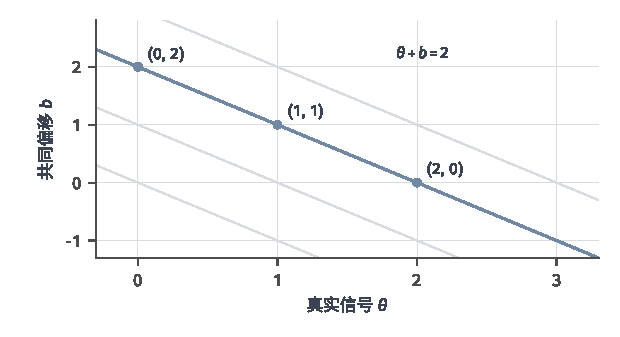
\includegraphics[width=105mm]{figures/00-shared/mathematical-preliminaries-lower/01-random-variables-distributions-and-causality/matplotlib/probability-common-bias-identification/figure.pdf}
  \caption{共同偏移模型中的等价参数。模型为\(Y_i=\theta+b+\varepsilon_i\)，\(\varepsilon_i\)相互独立且服从\(\mathcal N(0,1)\)。蓝线上的参数均满足\(\theta+b=2\)，三个标记点\((0,2),(1,1),(2,0)\)产生相同的任意样本量观测联合分布；浅灰线仅辅助比较其他参数和。}
  \label{fig:probability-common-bias-identification}
\end{figure}

不可识别还直接限制任何估计程序。对赋范目标空间，若在每个允许的样本量\(n\)下都有
\(P_{\vartheta_1}^{(n)}=P_{\vartheta_2}^{(n)}\)，但
\(\tau(\vartheta_1)\neq\tau(\vartheta_2)\)，取两目标值距离的三分之一为
\(\epsilon>0\)。任何只依赖样本的估计量\(\widehat\tau_n\)在两种机制下具有相同
分布，因而不可能同时满足
\[
  \mathbb{P}_{\vartheta_j}
  \left\{\lVert\widehat\tau_n-\tau(\vartheta_j)\rVert<\epsilon\right\}
  \longrightarrow1,\qquad j=1,2.
\]
因为两个半径为\(\epsilon\)的球不相交，同一个估计量分布不可能把趋近于一的概率
同时赋给它们。这证明了：不可识别目标不能靠增加同类样本在全部等价机制下一致恢复。

\subsection{抽样与观测机制下的识别条件}
\subsubsection{抽样制度与目标总体}
\label{sec:statistics-sampling-population}
\label{sec:statistics-missingness-observation}
% Baseline T:127-251
统计结论必须先回答“想对谁成立”。\term{目标总体}（target population）是推断希望
覆盖的对象、时间和条件的集合；\term{抽样制度}（sampling regime）描述观测如何从
这些对象产生。若样本只来自工作日的一个传感器，模型本身不能把结论自动推广到周末或
另一批设备。

独立同分布抽样把每个\(Y_i\)视为来自同一分布的独立重复。配对抽样则把
\((Y_{i,A},Y_{i,B})\)视为一个单位，例如同一对象在两种条件下的读数。若这些配对单位跨\(i\)独立，差值
\(D_i=Y_{i,A}-Y_{i,B}\)也跨\(i\)独立；把两列拆成\(2n\)个独立记录会丢失配对信息。
分层抽样预先按群组分别抽取，成组抽样则一次抽取整个设备、班级或用户群。两者的
独立单位和加权方式不同。

\paragraph{条件分母、相关性与信息量}
配对的收益取决于对内协方差：
\[
  \operatorname{Var}(D_i)
  =\operatorname{Var}(Y_{i,A})+\operatorname{Var}(Y_{i,B})
   -2\operatorname{Cov}(Y_{i,A},Y_{i,B}).
\]
正协方差会降低差值方差，负协方差则可能使配对更差；“同一对象测两次”本身并不保证
精度提高。

设目标总体中群组\(g\)的比例为\(\pi_g\)，群组均值为\(\mu_g\)，则总体均值为
\[
  \mu=\sum_g\pi_g\mu_g.
\]
总体指标可能很好，却掩盖某个小群组的严重误差。若群组中有\(n_g\)个独立Bernoulli
结果，样本比率\(\widehat p_g\)的方差为
\[
  \operatorname{Var}(\widehat p_g)
  =\frac{p_g(1-p_g)}{n_g}.
\]
这里把\(n_g\)视为固定正整数。若观测对\((G_i,Y_i)\)独立同分布，且\(Y_i\mid G_i=g\)服从Bernoulli规律，群组样本数
\(N_g=\sum_i\mathbb{I}\{G_i=g\}\)也是随机的，则
\(\widehat p_g\)只在\(N_g>0\)时有定义，且上述方差是给定\(N_g\)后的条件方差；
无条件误差还要平均随机分母，并处理\(N_g=0\)事件。不确定性由实际相关分母决定，
而不是总样本量\(n\)。报告群组公平性或来源质量时，应同时报告分母、抽样方式和区间，
不能只排列百分比。

已知入样概率时，权重可以把抽样分布重新接回目标总体。令\(S\in\{0,1\}\)表示一个
总体对象是否入样，\(\rho(Z)=\mathbb{P}(S=1\mid Z)\)，并假设
\(S\mathrel{\perp}Y\mid Z\)、\(\rho(Z)>0\)以及
\(\mathbb{E}[|Y|/\rho(Z)]<\infty\)。条件期望给出
\[
  \mathbb{E}\left[\frac{SY}{\rho(Z)}\right]
  =\mathbb{E}\left[
    \frac{\mathbb{E}[S\mid Y,Z]Y}{\rho(Z)}
  \right]
  =\mathbb{E}[Y].
\]
这条逆概率恒等式恢复的是明确的总体平均。若某一区域\(\rho(Z)=0\)，或者入样在给定
\(Z\)后仍依赖未观测的\(Y\)，等式便不能仅由已记录部分的分布推出。

记录数也不等于独立信息量。若同一来源复制一条记录十次，样本平均的显示分母增大，
实际信息却没有增加。时间序列中的相邻读数可能共享漂移；群组内记录可能共享设备偏差。
这类依赖应通过按群组建模、块抽样或
\BookSectionRef{sec:stoch-markov-long-run-average}{第~\ref{sec:stoch-markov-long-run-average}节}的相关过程工具处理，而不能
继续套用独立样本方差。

时间抽样还会改变目标本身。若传感器每分钟记录一次，朴素平均直接对应的是当天这组分钟网格时刻的平均读数。若目标是全天连续均匀时刻的平均，有限网格还只是积分近似；网格逐渐变细且读数路径可作Riemann积分时，等间隔平均才逼近该目标。若只在告警后加密采样，朴素平均通常会过度代表异常时段。
一种修正方式是记录每个目标时段被抽中的概率并作逆概率加权，但这要求这些时段都有正的入样概率。完全未覆盖的夜间时段不能靠增大已有权重恢复。抽样日志因此也属于推断所需的观测记录。

抽样制度与分析单位应在看结果前确定。假设十台设备各产生一千条记录，而处理实际随机
分配给设备，那么有效随机化单位是十台设备，不是一万条记录。记录内噪声可以帮助估计
每台设备的均值，却不能把处理效应的独立单位扩充到一万。这个区别会同时影响标准误、
置换方式和训练测试划分。

\subsubsection{缺失与选择下的目标恢复}

不完整观测带来另一类问题。令\(R=1\)表示\(Y\)被观察到，\(X\)为始终可见变量。
若高读数更容易被漏记，仅分析留下的记录就会低估总体温度。要判断观测子样本能否用于原目标，需说明缺失是否与完整数据有关，或者这种关系能否被始终可见的协变量解释。下面三种机制正是按这一依赖是否存在、能否由已见信息消除来区分。
\term{完全随机缺失}（missing completely at random, MCAR）要求
\[
  R\mathrel{\perp}(X,Y).
\]
\term{随机缺失}（missing at random, MAR）要求
\[
  R\mathrel{\perp}Y\mid X,
\]
即给定已观测协变量后，缺失概率不再依赖缺失值本身。
\term{非随机缺失}（missing not at random, MNAR）则允许这种剩余依赖。

多个变量可能按不同模式缺失，此时“已观测变量”随模式改变，不能用一个固定条件集概括全部MAR要求。
\begin{definition}[观测模式与缺失机制]
  \label{def:statistics-missingness}
  设完整数据为\(\bm Z=(Z_1,\ldots,Z_d)\)，观测指示\(\bm R\in\{0,1\}^d\)。对每种模式\(\bm r\)，定义
  \[
    O(\bm r)=\{j:r_j=1\},\qquad M(\bm r)=\{j:r_j=0\}.
  \]
  实际记录为\((\bm r,\bm Z_{O(\bm r)})\)。令\(g(\bm r\mid\bm z)\)为给定完整数据时的模式概率核。若对每种\(\bm r\)都存在只依赖已见坐标的可测函数\(g_{\bm r}\)，使
  \[
    g(\bm r\mid\bm z)=g_{\bm r}(\bm z_{O(\bm r)})
  \]
  对完整数据分布几乎处处成立，则称机制为MAR。若\(g(\bm r\mid\bm z)\)对全部模式均不依赖\(\bm z\)，则为MCAR；若MAR条件失败，则为MNAR。
\end{definition}
例如在二维数据中，模式\((1,0)\)的出现概率可依赖\(Z_1\)，却不能依赖未见的\(Z_2\)；模式\((0,1)\)反过来可以依赖\(Z_2\)，却不能依赖\(Z_1\)。这是对每种模式分别施加的条件，不能只在当前观测到的某一模式上核对。“随机缺失”也不等于“缺失标记完全随机”，后者对应更强的MCAR。

当\(\mathbb{P}(R=1)>0\)时，MCAR下完整案例仍代表总体，但效率降低。MAR下可建模
\(\mathbb{P}(R=1\mid X)\)并加权，或建模\(Y\mid X\)后插补；两者都依赖模型和
正值条件。MNAR下的目标通常不能只由已记录部分的分布识别，需要机制假设、外部信息或敏感性分析。
MAR描述的是缺失概率依赖哪些变量，并不意味着可以丢弃所有不完整记录。
“缺失机制可忽略”则要指定在哪一种推断计算中省去机制项；定义似然后，
式~\eqref{eq:statistics-missing-likelihood}将说明这种省略还需要哪些参数条件。
数据表中的一个缺失标记本身不能证明属于哪种机制。

识别障碍在有界结果上已经出现。若\(0\leq Y\leq1\)且
\(\mathbb{P}(R=0)>0\)，观测数据只给出已见部分的\(RY\)与缺失指示；把所有未见
\(Y\)设为\(0\)或设为\(1\)会产生相同观测，却给出不同总体均值。因此不加机制条件
时只能得到
\[
  \mathbb{E}[RY]
  \leq\mathbb{E}[Y]
  \leq\mathbb{E}[RY]+\mathbb{P}(R=0).
\]
两个端点分别可由把全部未见结果设为\(0\)或\(1\)达到，所以仅凭上述信息不能继续
收紧。若MAR成立，并令
\(\pi(X)=\mathbb{P}(R=1\mid X)>0\)，则第
~\ref{sec:statistics-sampling-population}节的逆概率恒等式在这里化为
\[
  \mathbb{E}\left[\frac{RY}{\pi(X)}\right]
  =\mathbb{E}[Y].
\]
正值条件负责覆盖，条件独立负责把未见结果接回已见结果；权重很大时，即使目标可识别，
有限样本方差仍可能很高。
\begin{example}[贯穿本章的传感器校准数据]
\label{ex:statistics-running-sensor-calibration}
考虑教学构造的\(25\)个独立传感器响应，暂以高斯位置模型描述，单次噪声标准差已知为
\(\sigma=2\)，样本汇总为
\[
\overline y=10.4,\qquad
\frac1{25}\sum_{i=1}^{25}(y_i-\overline y)^2=4.
\]
若另问响应如何随校准输入\(x\)变化，靠近左边界\(x_0=0\)的三个观测为
\[
(x_i,y_i)=(0,9),(1,11),(3,13),
\]
在给定带宽下核权重为\(1,0.75,0.25\)。后面的局部回归、Bootstrap、区间与预测复用这些输入，只改变所报告的目标。它们是可核算的教学数值，不是实测性能报告；把局部输入关系加入模型时，也不再把全部读数视为同一位置分布的重复抽取。
\end{example}

\section{参数与函数的估计}
\label{sec:stats-parameter-inference-efficiency}
目标能够由观测规律确定后，有限记录仍只提供它的近似。估计一个均值时，输出是一个数；估计分布或条件函数时，输出是一整条规律。两种输出都可以采用参数化或非参数化构造：样本平均无须预设分布族，完整的高斯分布却可以由均值和方差确定。下面按输出对象展开，再说明似然、矩、损失与先验如何产生估计规则。

\subsection{有限维目标的估计}
\subsubsection{基于似然的参数估计}
\label{sec:statistics-likelihood-robustness}
\label{sec:statistics-bayes-hierarchy}
% Baseline T:266-439
同一组已见记录可以放在不同候选参数下评价：模型在这些记录处的概率质量或密度有多大？保持数据不变、让候选参数变化，就得到拟合所需的比较函数。它使用的是观测模型的质量或密度，而不是给参数直接分配概率。
给定观测\(\bm{y}\)后，\term{似然}（likelihood）
\[
  L(\vartheta;\bm{y})=p_\vartheta(\bm{y})
\]
相对于模型共同的参考测度定义，把数据固定，把参数看作待比较的变量。似然不是参数的
概率分布；只有再指定先验并归一化后，才得到后验分布。最大似然估计选择
\(\widehat\vartheta_{\mathrm{MLE}}\in\argmax_\vartheta L(\vartheta;\bm{y})\)，
通常等价于最小化负对数似然\scite{vanderVaart1998asymptotic}。

现在可以明确前面的缺失机制可忽略性。以连续数据为例，令\(p_\theta\)描述完整数据，
\(g_\psi\)描述缺失模式；\(\theta\)与\(\psi\)分别是两者的参数。若整个模型满足MAR，
固定已见模式\(\bm r\)与坐标\(\bm z_{\mathrm{obs}}\)后，观测似然分解为
\begin{equation}
\begin{aligned}
 L_{\mathrm{obs}}(\theta,\psi)
 &=\int p_\theta(\bm z_{\mathrm{obs}},\bm z_{\mathrm{mis}})
       g_\psi(\bm r\mid\bm z_{\mathrm{obs}})\,\mathrm d\bm z_{\mathrm{mis}}\\
 &=g_\psi(\bm r\mid\bm z_{\mathrm{obs}})
       L_{\mathrm{data}}(\theta),\\
 L_{\mathrm{data}}(\theta)
 &=\int p_\theta(\bm z_{\mathrm{obs}},\bm z_{\mathrm{mis}})
       \,\mathrm d\bm z_{\mathrm{mis}}.
\end{aligned}
\label{eq:statistics-missing-likelihood}
\end{equation}
离散坐标把相应积分换成求和。若参数域是直积\(\Theta\times\Psi\)，即两组参数可独立变化，
在机制因子为正的观测上比较\(\theta\)的似然时便可省去这个不含\(\theta\)的因子。
这里省去的是机制模型的计算，保留的是对缺失坐标积分后的数据似然；直接删除不完整行
不是这项分解允许的操作。

用两个二元坐标可以把这一步算完。设每行的两个坐标独立同分布，
\(Z_{i1},Z_{i2}\sim\operatorname{Bernoulli}(\theta)\)，
第一列总被记录，第二列是否缺失只取决于第一列，因而机制不依赖缺失值本身，
满足MAR。按第二列求和后，观测似然成为
\[
  L_{\mathrm{obs}}(\theta,\psi)
  =g_\psi(\bm r\mid \bm z_{\mathrm{obs}})
   \prod_i\Bigl[\theta^{z_{i1}}(1-\theta)^{1-z_{i1}}\Bigr].
\]
机制因子不含\(\theta\)，所以比较\(\theta\)时可以略去它；
剩下的是对每一行第一列的似然，第二列缺失的行同样参与。
这正是“对缺失坐标积分”与“丢掉整行”的差别：前者保留了第一列的信息，
后者把它们一并舍弃，估计量一般不再无偏。
若缺失机制反过来依赖第二列自身的取值，上述分解失效，
仅用已见数据不足以恢复\(\theta\)，需要显式写出机制模型。

对\(Y_i\overset{\mathrm{iid}}{\sim}\mathcal{N}(\theta,\sigma^2)\)，且
\(\sigma^2>0\)已知，
\[
  -\log L(\theta;\bm{y})
  =\frac{1}{2\sigma^2}\sum_{i=1}^n(y_i-\theta)^2+C.
\]
对\(\theta\)求导并令其为零，得到
\(\widehat\theta=\overline y\)。同一个样本平均也可由矩估计得到：总体矩
\(\mathbb{E}_\theta[Y]=\theta\)，于是令样本矩\(\overline Y\)等于总体矩。
似然法依赖完整分布形式，矩估计只使用选定矩条件。

“令导数为零”只寻找内点候选，不保证最大值存在或唯一。例如独立Bernoulli观测的
似然为
\[
  L(p;\bm y)=p^{\sum_i y_i}(1-p)^{n-\sum_i y_i},\qquad p\in[0,1].
\]
当样本同时含有\(0\)和\(1\)时，唯一最大值是样本比例；全为\(1\)或全为\(0\)时，
最大值分别落在边界\(p=1\)或\(p=0\)。若错误地把参数域写成开区间\((0,1)\)，
边界数据甚至只有上确界而没有最大似然估计。

压缩数据会丢掉细节，但有时这些细节与目标参数无关。例如Bernoulli样本的排列不同，只要成功次数相同，似然关于\(p\)的依赖就相同。充分性要求这种“保留全部参数信息”在整个指定模型中成立。
\begin{definition}[充分统计量]
  \label{def:statistics-sufficient-statistic}
  设样本\(\bm Y\)与统计量\(T(\bm Y)\)取值于标准Borel空间。若存在概率核\(K(t,\cdot)\)，对每个\(\vartheta\in\Theta\)都是\(\bm Y\)给定\(T=t\)的正则条件分布版本，而且\(K\)不依赖\(\vartheta\)，则称\(T\)为该模型的\term{充分统计量}（sufficient statistic）。各条件分布的等式按相应\(P_\vartheta^T\)-几乎处处意义理解。
\end{definition}
它是在给定摘要后，样本其余部分不再携带关于参数的信息。在受同一个\(\sigma\)有限测度支配的模型中，若密度可分解为
\[
  p_\vartheta(\bm y)=g_\vartheta(T(\bm y))h(\bm y),
\]
则因子分解定理说明\(T\)对\(\vartheta\)充分。直观地说，给定
\(T(\bm Y)=t\)后，条件密度中的参数因子在归一化时抵消，剩余分布不含
\(\vartheta\)。在有限离散样本空间上，逆向关系也可直接算出。若
\(\bm Y\mid T=t\)的条件质量\(k(\bm y\mid t)\)不依赖参数，则
\[
  p_\vartheta(\bm y)
  =p_\vartheta^T(T(\bm y))k(\bm y\mid T(\bm y)),
\]
也得到所需分解。一般连续情形的条件分布可能集中在低维纤维上，不能把这个离散乘法式未经参考测度核对就当成普通密度恒等式；因子分解定理负责一般受支配模型中的等价性。高斯位置模型中，已知方差时
\(\sum_iY_i\)充分。充分性是相对于指定模型而言的；模型失配后，压缩掉的部分可能正好
暴露失配。

\subsubsection{基于经验准则的估计与稳健性}
似然以指定模型的对数密度作为拟合准则。若目标是中位数、希望减轻异常值影响，或不愿假定完整分布形状，就需要按目标另选样本准则。下面的表达把这些估计方法放在同一个框架中，但不同准则的总体最小点未必相同。
\begin{definition}[M估计]
  \label{def:statistics-m-estimator}
给定可测准则\(\rho(y,\vartheta)\)，当下面的最小点集合非空且存在可测选择时，\term{\(M\)估计}（M-estimation）是从中选出的一个可测统计量：
\[
  \widehat\vartheta
  \in\argmin_{\vartheta\in\Theta}
  \frac1n\sum_{i=1}^n\rho(Y_i,\vartheta).
\]
\end{definition}
准则可微且最优点位于参数域内点时，一阶必要条件是估计方程
\[
  \frac1n\sum_{i=1}^n\psi(Y_i,\widehat\vartheta)=0,
  \qquad
  \psi(y,\vartheta)=\nabla_\vartheta\rho(y,\vartheta).
\]
取平方准则\(\rho(y,\theta)=(y-\theta)^2/2\)，就有\(\psi(y,\theta)=\theta-y\)，每个残差的作用随绝对值线性增长。
若\(\mathbb E|Y|<\infty\)，绝对损失\(\rho(y,\theta)=|y-\theta|\)的总体风险有限，
其最小点则是中位数：目标函数的左右
方向导数分别由\(\mathbb{P}(Y<\theta)\)与\(\mathbb{P}(Y>\theta)\)决定，最优条件是
\(\mathbb{P}(Y\leq\theta)\geq1/2\)且
\(\mathbb{P}(Y\geq\theta)\geq1/2\)。因此平方与绝对准则即使使用同一批位置数据，
也在估计不同的总体泛函。

\(M\)估计的一致性需要把经验准则与总体准则连接起来。记
\[
  Q_n(\vartheta)=\frac1n\sum_{i=1}^n\rho(Y_i,\vartheta),
  \qquad
  Q(\vartheta)=\mathbb{E}[\rho(Y,\vartheta)].
\]
设\(Q\)有限，并在唯一点\(\vartheta^\star\)取得最小值，并且该最小值
分离，即对每个\(\epsilon>0\)，
\[
  \inf_{\lVert\vartheta-\vartheta^\star\rVert\geq\epsilon}
  Q(\vartheta)>Q(\vartheta^\star).
\]
若\(\sup_{\vartheta\in\Theta}|Q_n(\vartheta)-Q(\vartheta)|
\xrightarrow{\mathbb{P}}0\)，且近似优化误差
\[
  Q_n(\widehat\vartheta_n)-\inf_{\vartheta\in\Theta}Q_n(\vartheta)
  =o_{\mathbb{P}}(1),
\]
其中\(o_{\mathbb{P}}(1)\)表示该随机误差依概率趋于零，则
\(\widehat\vartheta_n\xrightarrow{\mathbb{P}}\vartheta^\star\)。证明只需比较准则：
在任意固定的\(\epsilon\)球外，总体准则有正间隔；当一致偏差和优化误差都小于该
间隔的适当分数时，经验近似最小点不可能位于球外。这里使用全参数域上的一致偏差和球外分离，不另需紧性。若只能在紧集上证明一致收敛，就还需控制估计点落在这些紧集之外的概率。总体最小点不唯一时，可在相应的集合分离条件下研究估计点到最小点集合的距离。

若真实分布\(P_0\)不属于\(\mathcal P\)，就不能把拟合参数直接解释为真实机制的参数。其总体对数损失目标是：
\begin{definition}[伪真参数]
  \label{def:statistics-pseudo-true-parameter}
相对于共同参考测度的模型密度\(p_\vartheta\)，假定所比较的\(\mathbb E_{P_0}\log p_\vartheta(Y)\)均有定义，且下列最大点集合非空。集合中的任一点
\[
  \vartheta^\star
  \in\argmax_\vartheta\mathbb{E}_{P_0}[\log p_\vartheta(Y)]
\]
称为该准则的\term{伪真参数}（pseudo-true parameter）。
\end{definition}
在经验准则一致逼近、总体极值唯一且分离等条件下，最大似然估计才趋向该点；多个最大点时须改为集合结论。它是模型族中按对数损失最接近
真实分布的点，不必等于科学问题中的真实量。估计量收敛并不自动证明模型正确。

\paragraph{稳健损失与影响函数}
为了限制异常残差的作用，可使用阈值\(c>0\)的Huber损失
\[
  \rho_c(r)=
  \begin{cases}
    r^2/2,& |r|\leq c,\\
    c|r|-c^2/2,& |r|>c,
  \end{cases}
  \qquad
  \psi_c(r)=
  \begin{cases}
    r,& |r|\leq c,\\
    c\operatorname{sign}(r),& |r|>c.
  \end{cases}
\]
这里\(\psi_c(r)=\rho_c'(r)\)是损失对残差\(r\)的导数。由于
\(\nabla_\theta\rho_c(y-\theta)=-\psi_c(y-\theta)\)，位置估计的参数梯度方程
整体乘以\(-1\)后，等价地写成
\(\sum_i\psi_c(y_i-\widehat\theta)=0\)。小残差仍按平方损失处理，大残差的贡献被截在
\(\pm c\)。代价是：即使高斯模型完全正确，较小的\(c\)也会舍弃一部分有效幅度信息。

总体准则确定估计目标，却没有说明少量异常观测会把它拉动多少。可以向分布\(P\)加入比例为\(\epsilon\)的单点污染，再考察目标的一阶变化。
\begin{definition}[影响函数]
  \label{def:statistics-influence-function}
  设\(T\)为定义在概率分布上的实值或向量值统计泛函，\(\Delta_z\)为全部质量集中在\(z\)的概率测度。假定充分小的正\(\epsilon\)所对应的污染分布仍在\(T\)的定义域内；若右侧极限存在且有限，定义\term{影响函数}（influence function）为
  \[ \operatorname{IF}(z;T,P)=\lim_{\epsilon\downarrow0}
    \frac{T((1-\epsilon)P+\epsilon\Delta_z)-T(P)}{\epsilon}. \]
\end{definition}
例如对均值泛函，\(\operatorname{IF}(z;T,P)=z-\mathbb E_PY\)：同样少量的污染，位置越远，拉动越大。下面先用标量估计方程说明这项敏感性。设统计泛函
\(T(P)\)由
\[
  \mathbb{E}_P[\psi(Y,T(P))]=0
\]
定义，并令\(P_\epsilon=(1-\epsilon)P+\epsilon\Delta_z\)。记
\(A=\mathbb{E}_P[\partial_\theta\psi(Y,T(P))]\neq0\)。假设估计方程在
\(\epsilon=0\)附近可微，微分可移入期望，且所跟踪的根在局部唯一。对
\(\mathbb{E}_{P_\epsilon}[\psi(Y,T(P_\epsilon))]=0\)在
\(\epsilon=0\)处隐式求导，得到
\[
  0=-\mathbb{E}_P[\psi(Y,T(P))]
    +\psi(z,T(P))+A\,T'(0),
\]
第一项为零，因此
\begin{equation}
  \operatorname{IF}(z;T,P)=T'(0)
  =-A^{-1}\psi(z,T(P)).
  \label{eq:statistics-influence-function}
\end{equation}
平方损失的位置影响随\(z\)无界，Huber得分则有界。多维参数时\(A\)是估计方程的
Jacobian矩阵，式~\eqref{eq:statistics-influence-function}要求该矩阵可逆；经验风险中它常表现为Hessian矩阵近似，但只有可微、局部可逆且估计根稳定时，
这种近似才成立。影响函数只描述污染比例在零附近的一阶敏感性，不是任意污染比例下的
误差上界；在回归中，截断残差也不会自动限制极端输入产生的高杠杆影响。

图~\ref{fig:statistics-huber-loss}区分损失本身与它的导数。大残差的Huber损失仍持续增加，并不是把异常观测删除；被限制的是单个残差进入位置估计方程的得分。把“损失增长较慢”直接说成“整个估计量的影响有界”，还需要式~\eqref{eq:statistics-influence-function}中的局部曲率与输入条件。

\begin{figure*}[htbp]
  \centering
  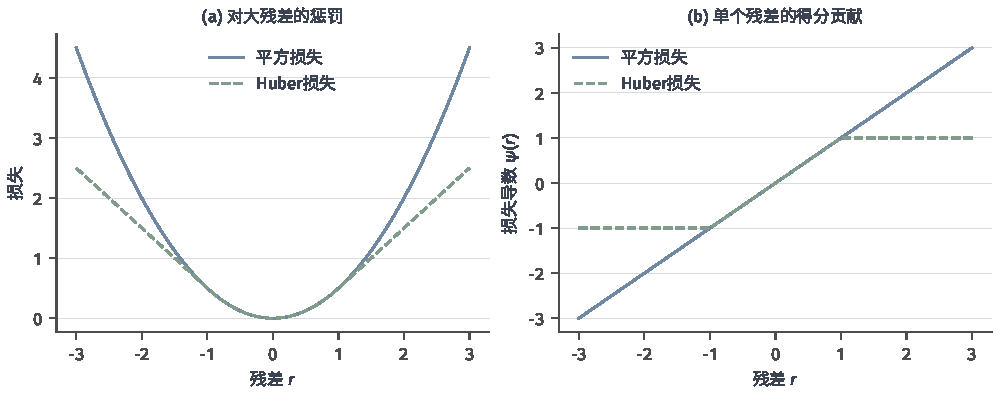
\includegraphics[width=\linewidth]{figures/00-shared/mathematical-preliminaries-lower/01-random-variables-distributions-and-causality/matplotlib/statistics-huber-loss/figure.pdf}
  \caption{平方损失与阈值\(c=1\)的Huber损失（解析式教学图）。左图比较惩罚值，右图比较对残差的导数；Huber得分在\([-1,1]\)内截断。横轴是构造残差，不代表实测异常值分布。}
  \label{fig:statistics-huber-loss}
\end{figure*}
\paragraph{污染模型与中位数的稳定性}
限制异常值影响之前，要先说明允许观测规律偏离到什么范围。常见的污染模型写成
\[
 P_\epsilon=(1-\epsilon)P_0+\epsilon Q,\qquad 0\leq\epsilon<1,
\]
其中\(P_0\)是希望拟合的主体规律，\(Q\)可为任意污染分布。目标若是\(P_0\)的位置参数，不能把\(P_\epsilon\)的均值自动当成该参数：即使污染比例很小，\(Q\)的尾部也能使均值偏移任意远，甚至不再存在。稳健准则必须同时说明希望保留的目标、允许的污染和所控制的误差\scite{huber1964}。

样本中位数能直接说明一种有限样本稳定性。取奇数个读数\(n=2k+1\)，把第\(k+1\)个顺序统计量作为中位数。若至多\(k\)条读数被任意替换，仍有至少\(k+1\)条未污染记录，因此中位数一定落在未污染读数的最小值与最大值之间：落在左侧或右侧都需要至少\(k+1\)条记录越过这个范围。替换\(k+1\)条则可把中位数推到任意远。对这个奇数样本约定，使估计值可以无界偏移的最小替换比例为\((k+1)/(2k+1)\)，趋近于\(1/2\)；均值只需替换一条，比例为\(1/n\)。这里讨论的是替换失效阈值，不是中位数对原位置参数的误差一定很小。

把同一计算用于局部窗口，就得到窗口中位数滤波。例如五个邻近读数为\((10,11,9,10,1000)\)，均值为\(208\)，中位数为\(10\)。这种收益依赖窗口内的主体值确实应当相近；窄峰、细线或边界附近的真实结构也可能被当作少数值抹去。它控制单个窗口内的排序敏感性，并不使相邻窗口输出独立。

\paragraph{基于最小子集的稳健模型拟合}
在直线或几何变换拟合中，异常匹配还可能具有极端输入位置，仅截断残差不能自动消除高杠杆影响。随机抽样一致性（random sample consensus, RANSAC）反复抽取足以确定模型的最小子集，生成候选参数，按预先指定的残差阈值找出相容记录，再用相容集重新拟合\scite{vision-ransac-1981}。阈值、最小子集大小和模型可识别性共同决定何种记录可算相容。

设每次随机抽样全为内点且能产生有效候选的概率至少为\(q\in(0,1)\)，不同轮次独立，连续\(K\)轮都未抽到这种子集的概率至多为\((1-q)^K\)。要求该失败概率不超过\(\delta\in(0,1)\)，足够取
\begin{equation}
 K\geq\left\lceil\frac{\log\delta}{\log(1-q)}\right\rceil.
 \label{eq:statistics-ransac-trials}
\end{equation}
若子集含\(m\)条独立内点标记、内点概率为\(w\)，且全内点子集总能确定有效模型，则\(q=w^m\)。从固定的\(n\)条记录中无放回抽取\(m\)条时，全内点概率应改为\(\binom{n_{\rm in}}m/\binom nm\)，其中\(n_{\rm in}\geq m\)；退化配置还会进一步降低有效概率。例如取独立标记模型的\(w=1/2,m=2,\delta=0.01\)，需\(K\geq17\)轮。

这个界只控制是否抽到有效内点子集。若阈值过宽、错误结构具有更大相容集，或全内点仍不能唯一确定模型，最终选择仍可能错误。用当前最大相容集的比例代替未知\(w\)只能得到依赖估计的停止规则，不能未经额外论证继续宣称上述确定概率保证。

\subsubsection{后验推断与层次汇聚}
% Baseline T:750-783
点估计只报告一个候选值，没有保留其他候选参数的不确定性。这个值可以是估计均值、中位数或其他目标的结果，不统一表示密度最大的参数位置。若还希望把已有的参数不确定性与新观测记录合在一起，可以先在候选参数上指定一张概率分布，再按各参数对这些记录的似然重新加权。Bayes更新沿这条路线产生参数的条件分布，所用先验是额外的建模条件。
频率学派把参数固定而把样本看作随机。Bayes方法另给参数指定先验
\(\pi(\theta)\)，观测后用
\[
  \pi(\theta\mid\bm y)
  =
  \frac{p(\bm y\mid\theta)\pi(\theta)}
       {\int p(\bm y\mid u)\pi(u)\,\mathrm du}
\]
得到\term{后验分布}（posterior distribution）。它把似然提供的数据证据与先验
假设合并。这个公式要求分母，即模型证据，严格为正且有限；否则右侧不能定义概率分布。

对式~\eqref{eq:statistics-missing-likelihood}中的两组参数，若先验还满足
\(\pi(\theta,\psi)=\pi_\Theta(\theta)\pi_\Psi(\psi)\)，则联合后验的未归一化密度分成
\[
 \{L_{\mathrm{data}}(\theta)\pi_\Theta(\theta)\}
 \{g_\psi(\bm r\mid\bm z_{\mathrm{obs}})\pi_\Psi(\psi)\}.
\]
在归一化常数严格为正且有限时，对\(\psi\)积分只产生与\(\theta\)无关的常数，
所以关于\(\theta\)的后验也可省去机制因子。这就是Bayes分析还需要先验可分离的含义；
若先验把两组参数联系起来，该因子一般会通过\(\psi\)影响\(\theta\)的后验\scite{pgm-parameter-learning-rubin1976}。

后验二阶矩有限时，后验均值最小化后验平方损失。事实上，对任意行动\(a\)，令
\(m=\mathbb{E}[\theta\mid\bm y]\)，则
\[
  \mathbb{E}[(\theta-a)^2\mid\bm y]
  =\operatorname{Var}(\theta\mid\bm y)+(a-m)^2.
\]
后验一阶绝对矩有限时，后验中位数则最小化后验绝对损失，其理由与前文总体中位数的左右方向导数相同。最大后验
估计只选择相对于指定参考测度的密度峰值；非线性重参数化会引入Jacobian因子，因此峰值
位置一般不保持不变。三种Bayes行动不必相同。

设
\[
  Y_i\mid\theta\overset{\mathrm{iid}}{\sim}\mathcal N(\theta,\sigma^2),
  \qquad
  \theta\sim\mathcal N(\mu_0,\tau_0^2).
\]
取\(\sigma^2,\tau_0^2>0\)。配方后得到共轭更新
\[
  \theta\mid\bm y
  \sim\mathcal N(\mu_n,\tau_n^2),\qquad
  \tau_n^{-2}=\tau_0^{-2}+n\sigma^{-2},
\]
\[
  \mu_n=\tau_n^2
  \left(\frac{\mu_0}{\tau_0^2}+\frac{n\overline y}{\sigma^2}\right).
\]
后验均值是先验均值与样本均值按精度加权的折中。新读数的后验预测还须加上观测噪声，见第~\ref{sec:statistics-scoring-calibration}节。
% Baseline T:792-834

离散比例也有同样的共轭结构。若
\(Y_i\mid p\overset{\mathrm{iid}}{\sim}\operatorname{Bernoulli}(p)\)且
\(p\sim\operatorname{Beta}(a,b)\)，观察到\(s=\sum_iY_i\)个成功后，
\[
  p\mid\bm y\sim\operatorname{Beta}(a+s,b+n-s).
\]
对\(K\)类计数\((n_1,\ldots,n_K)\)，Dirichlet先验
\(\operatorname{Dirichlet}(\alpha_1,\ldots,\alpha_K)\)相应更新为
\(\operatorname{Dirichlet}(\alpha_1+n_1,\ldots,\alpha_K+n_K)\)。这些更新依赖
给定比例后的条件独立抽样；过度离散或来源相关时，简单加计数会夸大信息量。

\paragraph{层次模型与部分汇聚}
多个设备、标注者或任务的数据量很不均衡时，可令
\[
  \theta_g\mid\mu,\tau^2\sim\mathcal N(\mu,\tau^2),\qquad
  Y_{g,i}\mid\theta_g\sim\mathcal N(\theta_g,\sigma_g^2).
\]
这里假设给定\((\mu,\tau^2)\)后各组参数\(\theta_g\)条件独立，并且给定全部组参数后，
所有\(Y_{g,i}\)也条件独立。若\(\mu,\tau^2,\sigma_g^2\)暂视为已知，\(\tau^2,\sigma_g^2>0\)，且第\(g\)组有
\(n_g\geq1\)个观测，则
\[
  \theta_g\mid\bm y_g,\mu,\tau^2
  \sim\mathcal N(m_g,V_g),\qquad
  V_g^{-1}=\tau^{-2}+n_g\sigma_g^{-2},
\]
\[
  m_g
  =V_g\left(\frac{\mu}{\tau^2}
    +\frac{n_g\overline y_g}{\sigma_g^2}\right).
\]
固定超参数时，第\(g\)组后验只依赖\(\bm y_g\)以及外部给定的共同中心和尺度；
小样本群组会更强地向共同中心\(\mu\)收缩，其他组数据尚未进入该后验。
当用全部群组数据估计共同超参数，或在完整Bayes模型中对其后验积分时，其他组数据才会
通过共同超参数间接改变第\(g\)组的推断，从而形成组间信息共享。
\(\tau^2\to0\)接近完全汇聚，\(\tau^2\to\infty\)接近各组独立估计，有限正尺度给出
部分汇聚。若超参数由同一数据估计，这是经验Bayes；若继续给它们指定先验，推断对象还
包括超参数后验。
这不是免费增加数据，而是加入“群组来自共同总体”的结构假设。若群组机制不同或先验
尺度过窄，收缩会掩盖真实差异。先验由研究者指定并不把固定物理参数变成随机生成的
事实；Bayes概率表达的是模型内部的不确定性。

有限维推断的目标也可以是一组总体分位数。设\(Y_1,\ldots,Y_n\)独立同分布且\(0<q<1\)，经验分布
\(\widehat F_n(y)=n^{-1}\sum_i\mathbb I_{\{Y_i\leq y\}}\)的广义逆给出
\(\widehat q=Y_{(\lceil nq\rceil)}\)。它估计的是总体分位数，不是未来读数的覆盖阈值；后者在共形预测中使用不同的秩修正。若总体在目标分位附近严格越过水平\(q\)，经验分布的统一收敛保证该估计一致；平坦区间、原子与不唯一目标则需按所选分位约定分析。

\subsection{分布与条件函数的估计}
\subsubsection{经验分布与密度估计}
\label{sec:statistics-nonparametric-missing}
经验分布把每个样本点赋质量\(1/n\)，因而是完整的概率分布而不是密度曲线。独立同分布样本下，Glivenko--Cantelli定理给出
\(\sup_y|\widehat F_n(y)-F(y)|\to0\)几乎必然；固定\(y\)的大数定律本身尚不等于这个统一结论。参数化方法则可报告\(P_{\widehat\theta}\)，例如
\(\mathcal N(\overline Y,S^2)\)，其有效性另外依赖模型限制。下面的平滑表示改变了分布或条件函数的形状，需要同时控制逼近误差与局部样本波动。
% Baseline T:1474-1583
有限维模型可能把真实分布限制得过强。非参数方法不预先固定有限个参数，但仍通过带宽、
邻域或平滑度控制复杂度。以下令\(Y_1,\ldots,Y_n\)独立同分布，具有同一个一维
密度\(f\)，并采用不依赖本批观测的带宽\(h=h_n>0\)。相关、选择或加权样本
需要另行计算期望与协方差，不能直接使用下面的独立样本公式。给定宽度为\(h\)的分箱，直方图用
“箱内样本数除以\(nh\)”作为箱内常数密度；移动箱边界可能改变估计。核密度估计则把
每个样本扩散为核：
\[
  \widehat f_h(x)
  =\frac1{nh}\sum_{i=1}^n
    K\left(\frac{x-Y_i}{h}\right).
\]
若\(K\geq0\)、积分为\(1\)，则\(\widehat f_h\)本身是非负且积分为\(1\)的密度。
为直接使用局部Taylor展开，以下采用一组充分条件：\(K\)非负、积分为\(1\)、有界、紧支撑且对称，
二阶矩记为\(\mu_2(K)=\int u^2K(u)\,\mathrm du\)，并记
\(R(K)=\int K(u)^2\,\mathrm du\)；两者均有限。设\(f\)在内部点\(x\)的邻域
二阶连续可微，则小带宽下核只涉及这个光滑邻域，由
\[
  \mathbb{E}[\widehat f_h(x)]
  =\int K(u)f(x-hu)\,\mathrm du
\]
作Taylor展开，核的一阶矩因对称性消失，从而得到
\[
  \operatorname{Bias}\{\widehat f_h(x)\}
  =\frac{h^2\mu_2(K)}2f''(x)+o(h^2),
\]
\[
  \operatorname{Var}\{\widehat f_h(x)\}
  =\frac{f(x)R(K)}{nh}+o((nh)^{-1}),
\]
其中渐近式取\(h\to0\)、\(nh\to\infty\)。较大带宽降低方差却增加平滑偏差。
边界附近因核质量落到支持集外，上述对称展开失效。
在\(d\)维中，体积因子变为\(h^d\)，代表性点态方差阶数相应为
\(1/(nh^d)\)。因此维数增加会更快消耗局部样本；一维的带宽结论不能不改条件直接
移植到高维。

\subsubsection{条件均值与分位数的估计}
这里的观测改为\((X_i,Y_i)_{i=1}^n\)，假定它们来自同一联合分布且独立同分布，
\(Y\)可积。采用前面核密度估计中的非负、有界、紧支撑核\(K\)与确定带宽\(h>0\)。
回归函数\(m(x)=\mathbb{E}[Y\mid X=x]\)可由局部平均估计；以下比值只在
权重和\(\sum_iK((X_i-x)/h)>0\)时定义：
\[
  \widehat m_h(x)=
  \frac{\sum_iK((X_i-x)/h)Y_i}
       {\sum_iK((X_i-x)/h)}.
\]
局部线性回归在\(x\)附近拟合\(a+b(X_i-x)\)，在相应平滑条件下可减轻设计
密度不均和边界偏差。下面的唯一拟合还要求局部加权设计满秩；在这个一维两参数问题中，
即正权重的输入至少含两个不同取值。若权重和为零或设计退化，需扩大邻域或另给退化处理，
不能照用比值或逆矩阵公式。
\[
  (\widehat a,\widehat b)
  \in\argmin_{a,b}\sum_{i=1}^n
  K\left(\frac{X_i-x}{h}\right)
  \{Y_i-a-b(X_i-x)\}^2,
  \qquad \widehat m_{\mathrm{local}}(x)=\widehat a.
\]
\(k\)近邻取\(1\leq k\leq n\)，用离\(x\)最近的\(k\)个样本平均；距离并列时
按预先指定的规则选择。维数增大时，为包含足够邻居必须扩大
邻域，Taylor局部性随之变差，这就是维数灾难的一种表现。

在例~\ref{ex:statistics-running-sensor-calibration}的左边界\(x_0=0\)，局部常数
估计为
\[
  \widehat m_h(0)
  =
  \frac{1\times9+0.75\times11+0.25\times13}
       {1+0.75+0.25}
  =10.25.
\]
局部线性拟合令\(u_i=x_i-x_0\)。由这三个点可算得
\[
  S_0=\sum_i w_i=2,\quad
  S_1=\sum_i w_i u_i=1.5,\quad
  S_2=\sum_i w_i u_i^2=3,
\]
\[
  T_0=\sum_i w_i y_i=20.5,\qquad
  T_1=\sum_i w_i u_i y_i=18.
\]
加权正规方程给出
\[
  \widehat a
  =\frac{S_2T_0-S_1T_1}{S_0S_2-S_1^2}
  =9.2,\qquad
  \widehat b
  =\frac{S_0T_1-S_1T_0}{S_0S_2-S_1^2}
  =1.4.
\]
因此局部线性预测为\(9.2\)，而局部常数预测为\(10.25\)。在边界处，后者只能对单侧
观测加权平均，前者还估计局部斜率并把直线截距放回\(x_0\)；哪一个更接近真实条件均值
仍取决于局部线性近似和带宽是否合适，不能由这一组数值单独决定。

图~\ref{fig:statistics-local-boundary-fit}显示这两个预测值的几何区别：水平线只改变高度，斜线同时解释输入位置与响应的局部变化，再把截距取回边界点。图中的观测和权重就是上面的三个教学数据；未画出未知的真实条件均值，因此不能从图上断言哪一种估计误差更小。
\begin{figure}[htbp]
  \centering
  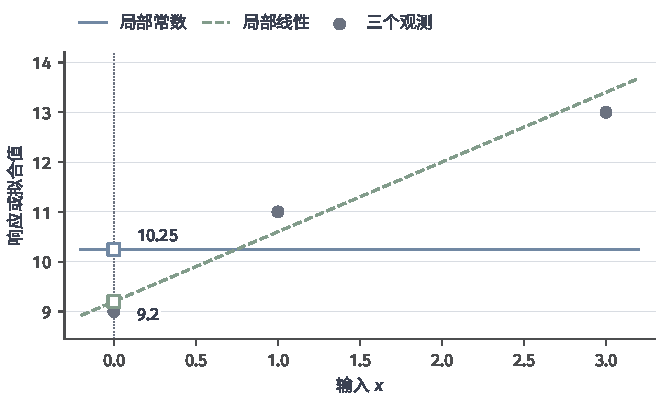
\includegraphics[width=\linewidth]{figures/00-shared/mathematical-preliminaries-lower/01-random-variables-distributions-and-causality/matplotlib/statistics-local-boundary-fit/figure.pdf}
  \caption{边界处的局部常数与局部线性拟合（教学数据图）。观测为\((0,9),(1,11),(3,13)\)，权重为\(1,0.75,0.25\)。蓝实线为加权常数\(10.25\)，绿虚线为\(9.2+1.4x\)，边界\(x_0=0\)处分别预测\(10.25\)和\(9.2\)。}
  \label{fig:statistics-local-boundary-fit}
\end{figure}

在上述独立同分布抽样下，这些方法的一致性需要邻域既缩小又包含越来越多样本。
例如一维内部点处，若输入密度在
\(x\)附近连续且为正，条件均值足够光滑，条件方差局部有界，并取
\(h\to0\)、\(nh\to\infty\)，局部常数估计的平滑偏差消失，局部平均的方差也消失。
输入密度与条件均值都二阶连续可微时，常用局部展开给出\(O(h^2)\)的平滑偏差
以及\(O((nh)^{-1})\)的方差，因此平滑偏差的平方为\(O(h^4)\)；精确常数还依赖
核、输入密度与条件噪声。近邻版本相应要求\(k\to\infty\)且\(k/n\to0\)。
这些都是目标分布有局部覆盖时的内插结论；在训练输入密度为零的区域，缩小邻域无法产生
新信息，外推保证必须来自额外结构假设。
% Baseline T:977-988
局部均值平均正负误差，不能直接给出较高的风险分位点。若报告值为\(a\)，低报时残差\(Y-a>0\)，高报时残差为负；希望估计较高分位数，就应让低报承担更大的单位代价。给定所求分位水平\(q\in(0,1)\)，下面用\(q\)与\(1-q\)分别加权这两侧绝对误差，再由左右导数核验最小点恰好满足分位数条件。
条件分位数可由\term{分位数回归}估计。假设\(Y\)可积，使下面损失的条件期望对几乎每个\(x\)有限。令
\[
  \rho_q(u)=u\bigl(q-\mathbb{I}_{\{u<0\}}\bigr),
\]
则条件\(q\)分位数最小化
\(\mathbb{E}[\rho_q(Y-a)\mid X=x]\)。固定\(x\)并记条件分布函数为\(F\)，目标对
\(a\)的次梯度区间是
\[
  [F(a^-)-q,\ F(a)-q].
\]
因此最优点恰好满足\(F(a^-)\leq q\leq F(a)\)；连续严格递增时才简化为
\(F(a)=q\)。因此分位数损失的最小点集合正是\(\mathcal Q_q\)，可能不唯一，
而\(F^{-1}(q)\)仍是其中按约定选出的单个代表。分位数回归直接估计条件分布的位置，
不要求误差为高斯或方差恒定。
实际分位数回归把条件分位函数写成\(a=f(x)\)，最小化
\(\sum_i\rho_q(Y_i-f(X_i))\)及可能的正则项。线性、样条或其他函数类限制决定了可表示的条件分位形状；最小化同一损失不意味着所有表示有同样的偏差与覆盖保证。

\section{未来观测的预测}
\label{sec:stats-prediction-observation-limits}
即使总体均值已知，下一次传感器读数仍会受新噪声影响。预测要把这种结果波动与估计未知规律的误差同时纳入。若先得到未来结果的分布，就能按所采用的损失选择报告内容：平方损失对应均值，绝对损失对应中位数，错判损失对应最可能类别；预测集合则保留一组结果并说明其覆盖概率。

\subsection{预测分布的计算与评价}
\label{sec:statistics-scoring-calibration}
若参数给定，条件预测使用概率核\(P_\theta(Y_{\rm new}\in\cdot\mid X_{\rm new}=x)\)；
代入估计得到插件预测，Bayes方法则对参数后验积分：
\[
P(Y_{\rm new}\in A\mid\bm y,x)
=\int P_\theta(Y_{\rm new}\in A\mid x)\,\pi(\mathrm d\theta\mid\bm y),
\]
这里假设给定参数后新观测与训练数据按模型条件独立。代入一个参数通常没有传播全部参数不确定性。
在前述高斯共轭模型中，
% Baseline T:784-790
\[
  Y_{n+1}\mid\bm y
  \sim\mathcal N(\mu_n,\sigma^2+\tau_n^2).
\]
其中\(\tau_n^2\)是参数不确定性，\(\sigma^2\)是新观测自身的噪声。
% Baseline T:1358-1467
点预测只给一个结果，概率预测则给出整个候选分布。若只奖励是否猜中最可能结果，报告完整概率并没有优势；评分必须鼓励把真实不确定性如实报告。
\begin{definition}[适当评分规则]
  \label{def:statistics-proper-scoring-rule}
  给定预测分布类\(\mathcal P\)，\term{评分规则}（scoring rule）\(S(Q,y)\)，即报告预测分布\(Q\)而结果为\(y\)
时承担的损失。假定所比较的期望均有定义，且诚实报告的期望有限。若对每个\(P,Q\in\mathcal P\)有\(\mathbb E_PS(P,Y)\leq\mathbb E_PS(Q,Y)\)，就称评分规则
\term{适当}（proper）；若适用分布类中的最小点唯一，则称为严格适当。
\end{definition}
它奖励诚实概率，而不是只检查最可能类别是否猜中。

对数评分的适当性直接回用第~\ref{chap:information-theory-and-statistical-geometry}章的KL散度及其非负性。下面取有限结果集\(\mathcal Y\)，用\(p,q\)表示真实分布与报告分布的概率质量函数；在真实分布赋正概率处报告零概率时，对数损失为正无穷。

离散结果的对数评分为\(S(Q,y)=-\log q(y)\)。根据上述定义，其期望差满足
\[
  \mathbb{E}_P[S(Q,Y)]-\mathbb{E}_P[S(P,Y)]
  =\sum_{y\in\mathcal Y}p(y)\log\frac{p(y)}{q(y)}
  =D_{\mathrm{KL}}(P\Vert Q)\geq0.
\]
因此对数评分是严格适当的；零预测概率遗漏真实分布的支持时，期望损失为无穷。
连续密度版本还要求相对于共同参考测度定义密度，并保证相关对数期望有定义；改变参考
坐标会改变单个对数密度值，但在合法换元下比较同一结果分布的期望差保持一致。

二元结果\(Y\in\{0,1\}\)的Brier评分为\(S(q,Y)=(q-Y)^2\)。若真实事件概率为
\(p\)，则
\begin{align}
  \mathbb{E}_p[(q-Y)^2]
  &=p(q-1)^2+(1-p)q^2\\
  &=(q-p)^2+p(1-p).
\end{align}
第二项与报告\(q\)无关，所以唯一最优报告是\(q=p\)。对数评分更强烈惩罚对已发生
事件给极小概率，Brier评分则有界；两者对预测误差采用不同的惩罚尺度。

对\(K\)个类别，令真实概率向量为\(\bm p\)，报告为\(\bm q\)，Brier评分可写成
\(S(\bm q,Y)=\sum_{k=1}^K(q_k-\mathbb{I}\{Y=k\})^2\)。直接展开得到
\[
  \mathbb{E}_{\bm p}[S(\bm q,Y)]
  =\lVert\bm q-\bm p\rVert_2^2
   +1-\lVert\bm p\rVert_2^2.
\]
所以它在概率单纯形上同样严格适当，但控制的是概率向量的平方距离，不是对数密度比。

\paragraph{校准、区分能力与锐度}
适当评分鼓励如实报告概率，但实际得到的预测器是否做到了，仍需在评价总体上检查。例如，把所有报告\(0.8\)的预测归在一起，这些结果为\(1\)的比例是否也为\(0.8\)？校准将这种按报告概率分组后的频率要求写成条件期望；它不是逐个样本都预测正确的要求。
\begin{definition}[二元概率校准]
  \label{def:statistics-probability-calibration}
  设\(Y\in\{0,1\}\)，预测概率为随机变量\(Q\in[0,1]\)。若
  \[ \mathbb E[Y\mid Q]=Q\quad\text{几乎必然}, \]
  则称预测相对于当前联合总体分布是\term{校准}（calibration）的。等价地，\(\mathbb P(Y=1\mid Q=q)=q\)对\(P_Q\)-几乎每个\(q\)成立。
\end{definition}
它要求预测概率相同的一组样本具有相应的真实发生率，而不要求有限样本中每组频数恰好等于预测值。\term{区分能力}（discrimination）描述模型
能否给更可能发生事件的样本更高分；\term{锐度}（sharpness）描述预测分布是否集中。
对所有样本恒报基准发生率可以完美校准，却没有区分能力。评价锐度时还要检查校准，否则更集中的预测可能只是过度自信。

令\(Q=\widehat p(X)\)、\(\eta(Q)=\mathbb{E}[Y\mid Q]\)，再记总体发生率为
\(\overline p=\mathbb{E}[Y]\)。条件平方展开给出
\[
  \mathbb{E}[(Q-Y)^2]
  =
  \underbrace{\mathbb{E}[(Q-\eta(Q))^2]}_{\text{校准误差}}
  +\underbrace{\overline p(1-\overline p)
    -\operatorname{Var}(\eta(Q))}_{\text{剩余不可分辨误差}}.
\]
第一项为零才表示相对于预测值本身校准；第二项随不同预测组的真实风险更可区分而减小。
恒报\(\overline p\)使第一项为零，却也使
\(\operatorname{Var}(\eta(Q))=0\)。多类别校准相应要求
\(\mathbb{P}(Y=k\mid\widehat{\bm p})=\widehat p_k\)对每个类别成立，逐类别边际校准
通常弱于这个向量条件。

一个固定的两组例子可以把这几个性质分开。设两组各占总体一半，事件概率分别为\(0.2,0.8\)。如表~\ref{tab:statistics-calibration-discrimination}，恒报\(0.5\)和按组报\(0.2,0.8\)都校准；前者把两组混在一起，后者保留了风险差异。按组报\(0,1\)保持相同排序，预测更集中，却把仍可能发生的意外结果说成不可能。
\begin{table}[htbp]
  \centering
  \small
  \begin{tabular}{lccc}
    \toprule
    报告规则 & 两组概率 & 总体校准 & 期望Brier损失 \\
    \midrule
    恒报总体发生率 & \(0.5,0.5\) & 是 & \(0.25\) \\
    如实报告组风险 & \(0.2,0.8\) & 是 & \(0.16\) \\
    只保留确定类别 & \(0,1\) & 否 & \(0.20\) \\
    \bottomrule
  \end{tabular}
  \caption{同一个两组总体下的校准与区分能力。数值由\(\mathbb E[(q-Y)^2]=(q-p)^2+p(1-p)\)逐组平均得到；后两行的类别排序相同，但概率准确性不同。}
  \label{tab:statistics-calibration-discrimination}
\end{table}

\paragraph{后处理校准与评价条件}
设分类器为\(K\)个类别输出实数分数\(z_1,\ldots,z_K\)，这些尚未归一化的分类分数称为logit。
softmax将它们变为概率\(q_k=\exp(z_k)/\sum_{j=1}^K\exp(z_j)\)。温度缩放改用
\(q_k(T)=\exp(z_k/T)/\sum_j\exp(z_j/T)\)，在校准集上按对数损失估计\(T>0\)。
例如分数\((2,0)\)在\(T=1\)时给第一类约\(0.881\)的概率，在\(T=2\)时约为\(0.731\)。
正温度保持类别排序，改变概率的集中程度；这种调整本身不保证总体校准。保序回归则拟合单调的分数到概率映射，更灵活但更容易在小
校准集上过拟合。把分数按\(s_1\leq\cdots\leq s_m\)排序后，其典型拟合问题是在
\(q_1\leq\cdots\leq q_m\)约束下最小化
\(\sum_i(q_i-y_i)^2\)；相同分数还须取相同拟合值，或先合并这些记录；单调约束不等于总体校准保证。
训练原预测器、拟合校准器和评价校准效果应使用职责分离的数据或严格的折外预测；
部署总体若发生变化，旧映射也未必保持校准。分箱可靠性图只是把连续条件近似成有限组，
箱内比例仍有抽样误差，且结果依赖分箱边界。适当评分、边际覆盖和校准分别评价分布损失、
未来集合与条件发生率，不能互相替代。

\subsection{预测集合的构造与覆盖}
\label{sec:probability-exchangeability-conformal-ranks}
\label{sec:rv-prediction-sets}
预测集合\(C(\bm Y)\)在规定的训练数据与未来观测联合规律下要求
\(\mathbb P\{Y_{n+1}\in C(\bm Y)\}\geq1-\alpha\)，其中\(0<\alpha<1\)。
在独立高斯位置模型\(Y_i\sim\mathcal N(\theta,\sigma^2)\)且\(\sigma\)已知时，
\[
Y_{n+1}-\overline Y\sim\mathcal N(0,\sigma^2(1+1/n)).
\]
因为新噪声与训练均值独立，方差中除了估计均值的\(\sigma^2/n\)，还有新观测的\(\sigma^2\)。因此
\[
C(\bm Y)=\left[\overline Y-z_{1-\alpha/2}\sigma\sqrt{1+1/n},
\overline Y+z_{1-\alpha/2}\sigma\sqrt{1+1/n}\right].
\]
这里\(z_p\)是标准高斯分布的下\(p\)分位数。取\(1-\alpha=0.95\)，
例~\ref{ex:statistics-running-sensor-calibration}的数值给出
\([6.40,14.40]\)。方差未知但仍为高斯独立样本时，可用
\(\overline Y\pm t_{n-1,1-\alpha/2}S\sqrt{1+1/n}\)获得精确预测区间。
其中\(n\geq2\)，\(S^2=(n-1)^{-1}\sum_i(Y_i-\overline Y)^2\)，
\(t_{\nu,p}\)为自由度\(\nu\)的Student \(t\)分布下\(p\)分位数。
该分布是独立的\(Z\sim\mathcal N(0,1)\)与\(U\sim\chi_\nu^2\)所成比值
\(Z/\sqrt{U/\nu}\)的规律。要在这里使用它，须把样本分成独立的均值方向和残差方向。

\begin{lemma}[高斯样本的均值与残差分解]
\label{lem:statistics-gaussian-mean-residual}
设\(n\geq2\)、\(\sigma>0\)，且\(Y_1,\ldots,Y_n\)独立同分布于
\(\mathcal N(\theta,\sigma^2)\)。则
\[
 Z_0=\frac{\sqrt n(\overline Y-\theta)}{\sigma}\sim\mathcal N(0,1),
 \qquad U=\frac{(n-1)S^2}{\sigma^2}\sim\chi^2_{n-1},
\]
且\(Z_0\)与\(U\)独立。
\end{lemma}
\begin{proof}
将标准化样本写成\(\bm\varepsilon=(\bm Y-\theta\bm1)/\sigma\sim\mathcal N(\bm0,\bm I_n)\)。
选择首行为\(\bm1^\top/\sqrt n\)的正交矩阵\(\bm Q\)；其余行构成与\(\bm1\)正交的残差方向。
向量\(\bm V=\bm Q\bm\varepsilon\)仍服从\(\mathcal N(\bm0,\bm I_n)\)，
所以各坐标是独立标准高斯。第一坐标\(V_1=Z_0\)；
正交变换保持长度，并把常量方向与其正交补分开，故
\[
 \sum_{j=2}^nV_j^2
 =\left\|\bm\varepsilon-\frac{\bm1\bm1^\top}{n}\bm\varepsilon\right\|_2^2
 =\frac1{\sigma^2}\sum_{i=1}^n(Y_i-\overline Y)^2=U.
\]
因此残差平方和具有\(n-1\)个自由度，并与第一坐标独立。
\end{proof}
新观测\(Y_{n+1}\)独立于全部训练样本，所以\((Y_{n+1},\overline Y)\)与\(S\)独立，
且\((Y_{n+1}-\overline Y)/(\sigma\sqrt{1+1/n})\)是标准高斯。
将它与上述\(U\)代入\(t\)分布定义，就得到所用的精确预测区间。
这类保证依赖参数模型；只愿假设可交换性时，可改用下面的秩方法。
% Baseline P:2293-2356
设实值分数\(S_1,\ldots,S_{m+1}\)可交换，并暂假它们几乎必然没有并列值。令
\[ R_{m+1}
  =1+\sum_{i=1}^{m}\mathbb{I}\{S_i<S_{m+1}\} \]
为最后一个分数从小到大的秩。由于交换任意两个坐标不改变联合分布，而无并列值时每个样本恰占一个秩，所以
\begin{equation}
  \mathbb{P}(R_{m+1}=r)=\frac{1}{m+1},
  \qquad r=1,\ldots,m+1.
  \label{eq:probability-uniform-rank}
\end{equation}
这是一项精确的有限样本结论，不依赖中心极限定理。

若存在并列值，使用“严格小于”的秩不再均匀。可以为每个分数附加独立连续随机数并按字典序打破并列，此时恢复精确均匀秩；也可以采用保守的不随机化分位数，得到覆盖率至少为目标值，但通常不再精确等于目标值。

\paragraph{拆分共形预测的有限样本覆盖}
设训练数据用于拟合一个固定预测规则，随后有\(m\)个校准样本和一个未来样本。条件于训练样本及拟合所用学习规则的随机性，假设校准样本与未来样本可交换。用同一个不一致性函数计算
\[ S_i=s(X_i,Y_i),
  \qquad i=1,\ldots,m+1. \]
分数越大表示候选标签与预测规则越不相容。给定错误率\(\alpha\in(0,1)\)，令
\[ k=\left\lceil(m+1)(1-\alpha)\right\rceil. \]
若\(k\leq m\)，令\(q\)为前\(m\)个校准分数的第\(k\)小值；若\(k=m+1\)，约定\(q=+\infty\)。对新输入\(X_{m+1}\)，定义预测集合
\begin{equation}
  C(X_{m+1})
  =
  \{y:s(X_{m+1},y)\leq q\}.
  \label{eq:probability-split-conformal-set}
\end{equation}

例如\(m=9\)、\(\alpha=0.2\)时，\(k=\lceil10\times0.8\rceil=8\)。若排序后的校准分数为
\(0.1,0.2,\ldots,0.9\)，则\(q=0.8\)：候选标签的分数为\(0.75\)时纳入集合，为\(0.85\)时排除。若仍只有九个校准样本却要求
\(\alpha=0.05\)，则\(k=\lceil9.5\rceil=10=m+1\)，按约定得到\(q=+\infty\)。这不是计算故障，而是有限样本不足以用非随机秩给出如此高的非平凡覆盖水平。

图~\ref{fig:probability-conformal-ranks}区分了阈值的执行与覆盖率的来源。上方固定刚才的九个教学校准值，展示候选标签怎样按分数与\(q\)比较；下方则回到校准分数与未来真实分数共同随机生成的无并列可交换设定，表示未来分数可能占据的十个等概率秩。前八个秩被覆盖，剩余两个秩构成不覆盖事件。均匀秩所平均的是这十个分数的联合随机性，并不是说给定图上这九个具体校准数值后，未来分数的条件秩仍然均匀。

\begin{figure}[htbp]
  \centering
  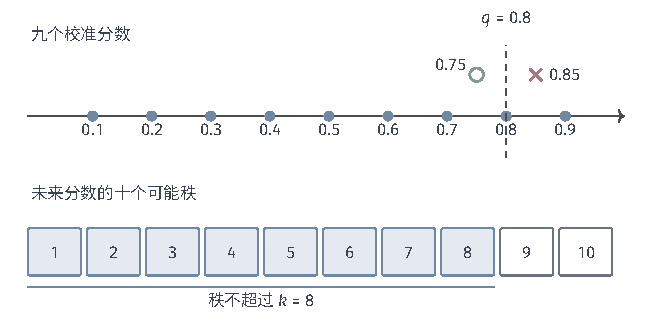
\includegraphics[width=111mm]{figures/00-shared/mathematical-preliminaries-lower/01-random-variables-distributions-and-causality/tikz/probability-conformal-ranks/source.pdf}
  \caption{拆分共形中的分数阈值与秩位置。上方取\(m=9\)、\(\alpha=0.2\)，校准值为\(0.1,\ldots,0.9\)，故\(k=8\)、\(q=0.8\)；空心圆候选分数\(0.75\)被纳入，叉号候选分数\(0.85\)被排除。下方浅色槽表示无并列可交换分数下未来秩不超过\(8\)的事件，其概率\(8/10\)针对校准与未来分数的联合抽样，而非给定上方校准值后的条件保证。}
  \label{fig:probability-conformal-ranks}
\end{figure}

\begin{theorem}[拆分共形的有限样本覆盖]
\label{thm:probability-split-conformal-coverage}
在上述条件下，
\[ \mathbb{P}\bigl(
    Y_{m+1}\in C(X_{m+1})\bigr)\geq 1-\alpha. \]
\end{theorem}

\begin{proof}
先假设分数无并列值。若未来真实标签未被覆盖，则\(S_{m+1}>q\)，所以未来分数在全部\(m+1\)个分数中的秩严格大于\(k\)。由式~\eqref{eq:probability-uniform-rank}，
\[ \mathbb{P}(S_{m+1}>q)
  =\mathbb{P}(R_{m+1}>k)=\frac{m+1-k}{m+1}\leq\alpha. \]
取补事件即得覆盖结论。

若有并列值，采用集合定义中的“\(\leq q\)”会把边界并列分数纳入预测集合。相较于随机打破并列后的精确秩，这只会增加覆盖事件，因此同一不等式仍成立。若希望得到更接近
精确的覆盖率，可显式随机化边界并列项，但必须把该随机化纳入算法与概率空间。
\end{proof}

这里的概率保证是\term{边际覆盖}：条件于训练数据后，它仍对随机的校准样本和未来样本共同取平均；若采用随机并列处理，还包括该随机性。解除对训练数据的条件后，总体覆盖率仍至少为
\(1-\alpha\)。但这个结论一般不推出对每个固定输入\(x\)都有
\[
  \mathbb{P}\bigl(
    Y_{m+1}\in C(X_{m+1})
    \mid X_{m+1}=x
  \bigr)
  \geq1-\alpha,
\]
也不自动保证每个群组内都达到同一覆盖率。逐输入、逐群组或时间条件覆盖需要额外结构、假设或专门的校准方法，不能仅由可交换秩推出。

证明依赖两处对称性。训练与校准拆分使评分规则在校准阶段保持固定；校准样本与未来样本可交换，使未来分数的秩没有特殊位置。若反复查看校准误差后修改模型或分数函数，评分规则
已依赖校准标签，条件可交换性可能被破坏。时间序列中的未来点通常也不能与过去点任意重排；自适应收集会让被选中的样本位置携带额外信息。此时失效的是均匀秩步骤，而不是把
分位数索引稍作调整就能修复。固定评分规则、校准与未来样本条件可交换时，本章的秩保证可以用于预测范围的边际覆盖；具体使用条件可参考
\BookChapterRef{chap:trust-reliability}{卷三的“可靠性”章}。
分组校准需要在看见校准结果前规定群组，并有足够的组内可交换样本。边际覆盖平均了输入位置，不自动给出每个连续输入处的条件覆盖。

\section{估计误差与效率}
\label{sec:stats-uncertainty-testing-selection}
一个估计数值需要评价平均损失或误差分布，一段参数范围需要评价重复抽样下的覆盖率，拒绝一个命题则需要控制误拒概率。评价标准由推断输出决定。重抽样、区间构造与检验程序都要在相应的抽样制度下建立保证；筛选数据或反复查看结果会改变该制度，因而必须重新核对条件。

\subsection{有限样本误差与线性估计效率}
\label{sec:statistics-bias-efficiency}
% Baseline T:446-459
估计量的误差既来自系统偏移，也来自样本波动。设标量估计量\(\widehat\theta\in L^2\)。对目标\(\theta\)，
\begin{align}
  \mathbb{E}[(\widehat\theta-\theta)^2]
  &=
  \mathbb{E}[(\widehat\theta-\mathbb{E}\widehat\theta
  +\mathbb{E}\widehat\theta-\theta)^2] \notag\\
  &=
  \operatorname{Var}(\widehat\theta)
  +\bigl(\mathbb{E}[\widehat\theta]-\theta\bigr)^2.
  \label{eq:statistics-mse-decomposition}
\end{align}
交叉项期望为零，因而均方误差等于方差加偏差平方。无偏不等于误差最小；少量偏差可能
换来更大的方差下降。

% Baseline T:470-498
若\(\bm\theta\in\mathbb{R}^d\)且\(\mathbb E\lVert\widehat{\bm\theta}\rVert_2^2<\infty\)，并使用总平方误差，则
\[
  \mathbb{E}\lVert\widehat{\bm\theta}-\bm\theta\rVert_2^2
  =\operatorname{tr}\{\operatorname{Cov}(\widehat{\bm\theta})\}
   +\lVert\mathbb{E}\widehat{\bm\theta}-\bm\theta\rVert_2^2.
\]
这不是每个坐标风险的最大值，也不是任意方向风险。

在高斯位置例子中，取固定中心\(\mu_0\)并令
\(\widetilde\theta=a\overline Y+(1-a)\mu_0\)，则
\[
  \operatorname{MSE}_\theta(\widetilde\theta)
  =\frac{a^2\sigma^2}{n}+(1-a)^2(\mu_0-\theta)^2.
\]
当\(\theta\)接近\(\mu_0\)时，某些\(a<1\)可比无偏的样本均值具有更小有限样本
均方误差；远离中心时，收缩偏差又可能占主导。比较结论必须固定目标、样本量和损失。

当任意\(\epsilon>0\)都满足
\(\mathbb{P}_\theta(|\widehat\theta_n-\theta|>\epsilon)\to0\)时，称估计量
\term{一致}（consistent）。一致性只描述样本量趋于无穷的极限，不给出当前样本的
误差，也不排除有限样本偏差。若
\(\mathbb{E}_\theta[(\widehat\theta_n-\theta)^2]\to0\)，则称为均方一致；
Markov不等式说明均方一致推出依概率一致，反向结论没有额外一致可积性时并不成立。
对某些满足额外正则条件的估计量，还能进一步证明
\[
  \sqrt n(\widehat\theta_n-\theta)
  \xrightarrow{\mathrm d}\mathcal N(0,V).
\]
这项性质称为渐近正态，它需要另行建立，并不由一致性自动推出。
% Baseline T:516-547
无偏性约束了平均位置，却尚未比较方差。把单一信号推广为一组带噪线性观测：给定设计矩阵\(\bm X\in\mathbb R^{n\times d}\)，设
\begin{equation}
  \bm Y=\bm X\bm\theta+\bm\varepsilon,\qquad
  \mathbb E[\bm\varepsilon\mid\bm X]=\bm0,\qquad
  \operatorname{Cov}(\bm\varepsilon\mid\bm X)=\sigma^2\bm I_n,
  \quad\sigma^2>0.
  \label{eq:statistics-gauss-markov-model}
\end{equation}
不同观测的条件噪声方差相同且协方差为零；这里不要求独立或高斯噪声。列满秩使参数可识别，最小二乘解为
\(\widehat{\bm\theta}=(\bm X^\top\bm X)^{-1}\bm X^\top\bm Y\)。它是否在所有无偏估计中最佳，需要先限定比较类。
\begin{theorem}[Gauss--Markov定理]
  \label{thm:statistics-gauss-markov}
  在式~\eqref{eq:statistics-gauss-markov-model}下，若\(\bm X\)列满秩，则\(\widehat{\bm\theta}\)条件无偏，且
  \(\operatorname{Cov}(\widehat{\bm\theta}\mid\bm X)=\sigma^2(\bm X^\top\bm X)^{-1}\)。
  对任何条件于\(\bm X\)固定、对全部\(\bm\theta\)均无偏的线性估计\(\widetilde{\bm\theta}=\bm C\bm Y\)，有
  \[
    \operatorname{Cov}(\widetilde{\bm\theta}\mid\bm X)
    -\operatorname{Cov}(\widehat{\bm\theta}\mid\bm X)\succeq\bm0.
  \]
\end{theorem}
\begin{proof}
记\(\bm C_0=(\bm X^\top\bm X)^{-1}\bm X^\top\)，于是\(\bm C_0\bm X=\bm I_d\)。直接对\(\bm C_0\bm Y\)求条件均值和协方差，得到无偏性及所述协方差。任一线性估计对所有参数无偏，等价于\(\bm C\bm X=\bm I_d\)。写\(\bm C=\bm C_0+\bm D\)，则\(\bm D\bm X=\bm0\)，从而
\[
  \bm C_0\bm D^\top
  =(\bm X^\top\bm X)^{-1}(\bm D\bm X)^\top=\bm0.
\]
展开\(\sigma^2\bm C\bm C^\top\)时两个交叉项都为零，故协方差之差为\(\sigma^2\bm D\bm D^\top\)。对任意向量\(\bm a\)，其二次型为\(\sigma^2\|\bm D^\top\bm a\|_2^2\geq0\)，即得半正定结论。
\end{proof}
半正定比较表示任意线性组合\(\bm a^\top\bm\theta\)的方差都不更大，强于只比较各坐标方差。定理的比较类是线性无偏估计，不排除前面那类有偏收缩估计获得更小均方误差，也不把异方差或相关噪声包含进来。

若\(\bm X=\bm1_n\)，参数就是共同均值，最小二乘退化为样本平均。任一无偏加权平均\(\sum_i a_iY_i\)满足\(\sum_i a_i=1\)；写\(a_i=1/n+b_i\)，则\(\sum_i b_i=0\)，其方差为
\(\sigma^2\sum_i a_i^2=\sigma^2/n+\sigma^2\sum_i b_i^2\)。额外的不均衡权重只增加方差，给出矩阵证明的一个可逐项核对的特例。
\subsection{渐近误差与估计方程的线性化}
% Baseline T:551-560
样本均值给出渐近正态的基本例子。若
\(Y_1,\ldots,Y_n\)独立同分布，且
\(\mathbb{E}[Y_i]=\theta\)、
\(0<\operatorname{Var}(Y_i)=\sigma^2<\infty\)，则中心极限定理给出
\[
  \sqrt n(\overline Y-\theta)
  \xrightarrow{\mathrm d}\mathcal N(0,\sigma^2).
\]
因此均值的渐近正态只需要有限方差，不要求观测本身服从高斯分布；在高斯位置模型中，
这个正态分布关系对每个有限\(n\)已经精确成立。
实际标准化常把未知方差换成样本估计。若样本方差一致，便可用\BookChapterRef{chap:random-sequences-and-processes}{第~\ref{chap:random-sequences-and-processes}章}的连续映射与Slutsky定理传递分布极限；这里只把这些运算用于估计误差，不重新建立一般收敛理论。

一般估计方程的渐近式还要控制在随机估计点附近的斜率。设\(Y_i\)独立同分布，且
\(\mathbb{E}[\psi(Y,\theta_0)]=0\)，记
\[
  A=\mathbb{E}[\partial_\theta\psi(Y,\theta_0)],
  \qquad B=\operatorname{Var}(\psi(Y,\theta_0)),
\]
要求\(A\neq0\)、\(B<\infty\)。一组足够条件是：\(\widehat\theta\)依概率趋于内点
\(\theta_0\)；\(\psi(y,\theta)\)在其某个邻域内连续可微；经验导数
\(n^{-1}\sum_i\partial_\theta\psi(Y_i,\theta)\)在该邻域上一致依概率收敛到
连续函数\(a(\theta)=\mathbb E[\partial_\theta\psi(Y,\theta)]\)；
估计方程残差\(r_n=n^{-1}\sum_i\psi(Y_i,\widehat\theta)\)满足
\(r_n=o_{\mathbb P}(n^{-1/2})\)。
一致性保证连接\(\theta_0\)与\(\widehat\theta\)的线段以趋于一的概率留在该邻域内。
沿线段积分导数，得到
\[
\begin{aligned}
 A_n&=\int_0^1\frac1n\sum_{i=1}^n
  \partial_\theta\psi\bigl(Y_i,\theta_0+t(\widehat\theta-\theta_0)\bigr)\,\mathrm dt
  \xrightarrow{\mathbb P}A,\\
 r_n&=\frac1n\sum_{i=1}^n\psi(Y_i,\theta_0)+A_n(\widehat\theta-\theta_0).
\end{aligned}
\]
随机斜率的收敛由一致导数控制与\(a\)的连续性共同给出，不能仅凭在固定点可微就断言。
因\(A\neq0\)，以趋于一的概率可以除以\(A_n\)；再由中心极限定理与Slutsky得到
\[
  \sqrt n(\widehat\theta-\theta_0)
  =
  -A^{-1}\frac1{\sqrt n}\sum_{i=1}^n\psi(Y_i,\theta_0)
  +o_{\mathbb{P}}(1),
\]
故极限方差为\(A^{-2}B\)，\(B=0\)时极限退化为零。多维情形将导数换为Jacobian，
要求其总体矩阵\(A\)非奇异，并对向量得分使用多元中心极限定理；极限协方差相应为
\(A^{-1}B(A^{-1})^\top\)，常称夹心协方差。模型正确的光滑似然在正则条件下可用
信息恒等式化简它；模型失配时\(A\)与\(B\)通常不再是同一个信息量，夹心两侧不能省略。

\subsection{Fisher信息与无偏估计的效率界}
均方误差评价一个给定估计量，效率界进一步询问同一观测模型允许的估计精度。
这里用对数似然的导数记录数据对参数的局部辨别能力；Fisher信息与统计几何章共用
同一个分布对象，定义见第~\ref{sec:information-fisher-geometry}节。本小节把得分用于无偏估计的误差下界。沿用标量得分\(u_\theta(y)=\partial_\theta\log p_\theta(y)\)，记\(\mathcal I(\theta)=\mathbb E_\theta u_\theta(Y_1)^2\)。独立样本的总得分为\(s_\theta(\bm Y)=\sum_{i=1}^n u_\theta(Y_i)\)；得分均值为零时，其方差为\(n\mathcal I(\theta)\)。

\begin{theorem}[Cramér--Rao下界]
\label{thm:statistics-cramer-rao}
设\(Y_1,\ldots,Y_n\)独立同分布于\(p_\theta\)，参数位于开区间，密度的支持不随参数改变，密度可对参数求导，归一化积分可交换求导与积分，得分的均值为零且方差等于Fisher信息。再设单样本
Fisher信息满足\(0<\mathcal I(\theta)<\infty\)。若\(\widehat\tau\)对可微目标
\(\tau(\theta)\)无偏、二阶矩有限，且其期望可对参数求导并移入积分，则
\[
  \operatorname{Var}_\theta(\widehat\tau)
  \geq\frac{\tau'(\theta)^2}{n\mathcal I(\theta)}.
\]
\end{theorem}

\begin{proof}
由无偏性\(\mathbb{E}_\theta[\widehat\tau]=\tau(\theta)\)对参数求导，并把导数移入积分，
得到
\[
  \tau'(\theta)
  =\mathbb{E}_\theta[
    (\widehat\tau-\tau(\theta))s_\theta(\bm Y)].
\]
Cauchy--Schwarz不等式给出
\[
  \tau'(\theta)^2\leq
  \operatorname{Var}_\theta(\widehat\tau)
  \operatorname{Var}_\theta(s_\theta(\bm Y))
  =
  \operatorname{Var}_\theta(\widehat\tau)n\mathcal I(\theta),
\]
整理即得结论。
\end{proof}

这个界不是所有估计问题的普遍极限。参数位于边界、支持依赖参数、模型不可识别或
Fisher信息奇异时，证明中的求导和除法可能失效；有偏估计量也要使用相应的偏差版本。
对\(\bm\theta\in\mathbb{R}^p\)和可微目标
\(\bm\tau(\bm\theta)\in\mathbb{R}^q\)，向量参数的正则版本为
\[
  \operatorname{Cov}_{\bm\theta}(\widehat{\bm\tau})
  \succeq
  \bm J_\tau(\bm\theta)\,
  \bm{\mathcal I}_n(\bm\theta)^{-1}\,
  \bm J_\tau(\bm\theta)^\top,
\]
其中\(\bm J_\tau\in\mathbb{R}^{q\times p}\)是目标映射的Jacobian，
\(\bm{\mathcal I}_n\)是整批样本的Fisher信息矩阵。这里要求信息矩阵可逆，
但Jacobian可以是矩形或降秩矩阵；估计参数本身时
\(\bm\tau(\bm\theta)=\bm\theta\)，故\(\bm J_\tau=\bm I_p\)。矩阵结论也不能由
逐坐标标量界直接拼接得到。
\section{区间估计与假设检验}
\label{sec:statistics-intervals-tests}
\subsection{区间估计的覆盖}
\subsubsection{固定样本下的覆盖与重抽样}
\label{sec:statistics-intervals-quantiles}
\label{sec:statistics-resampling}
% Baseline T:848-868
点估计没有说明误差尺度。覆盖区间需要先说明概率来自哪一次随机化，以及要覆盖的对象。
\begin{definition}[置信、可信与预测覆盖]
  \label{def:statistics-interval-coverage}
  取\(0<\alpha<1\)。\term{置信区间}（confidence interval）是一项重复抽样
程序：若每次按同一制度抽样并构造\(C(\bm Y)\)，则对模型中的每个\(\theta\)都有
\[
  \mathbb{P}_\theta\{\theta\in C(\bm Y)\}\geq1-\alpha.
\]
频率学派参数始终视作固定值；数据固定后，得到的区间也固定，不能把它解释为“以\(1-\alpha\)
概率包含参数”。Bayes\term{可信区间}（credible interval）则在给定数据和模型后
满足\(\mathbb{P}(\theta\in C\mid\bm y)\geq1-\alpha\)，其数值依赖先验；连续后验常可取到等号，离散后验可能只能给出更大的覆盖概率。
\term{预测集合}（prediction set）把覆盖对象改成未来结果，在规定的训练样本与未来
观测联合分布下要求
\(\mathbb{P}\{Y_{n+1}\in C(\bm Y)\}\geq1-\alpha\)。三者的概率分别来自重复样本、
参数后验，以及训练样本与未来观测的联合抽样，不能只按区间端点的外观解释。
\end{definition}

在独立同分布的高斯位置模型中，若方差已知，则
\[
  \frac{\overline Y-\theta}{\sigma/\sqrt n}\sim\mathcal N(0,1),
\]
% Baseline T:869-872
因而双侧置信区间为
\[
  \overline Y\pm z_{1-\alpha/2}\frac{\sigma}{\sqrt n}.
\]
这一区间覆盖固定均值，而第~\ref{sec:rv-prediction-sets}节的区间覆盖新观测。
取\(1-\alpha=0.95\)，对例~\ref{ex:statistics-running-sensor-calibration}，均值置信区间为
\[
10.4\pm1.96(2/5)=[9.62,11.18].
\]
它明显窄于下一次读数的预测区间\([6.40,14.40]\)，但不能替代后者。
% Baseline T:908-949

图~\ref{fig:statistics-mean-prediction-width}显示这一区分在样本量增长时仍然存在：均值标准误按\(n^{-1/2}\)减小，而未来单次读数的噪声不会因历史样本增多而消失。因此收集更多校准数据会把位置参数确定得更精确，却不能把一个有噪声的新读数限制到同样窄的范围。

\begin{figure}[!htb]
  \centering
  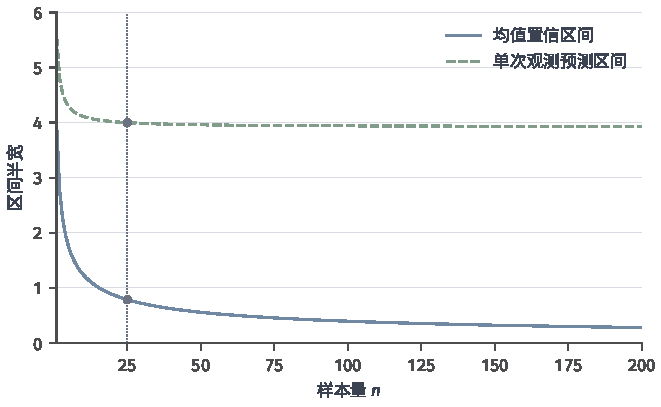
\includegraphics[width=\linewidth]{figures/00-shared/mathematical-preliminaries-lower/01-random-variables-distributions-and-causality/matplotlib/statistics-mean-prediction-width/figure.pdf}
  \caption{已知\(\sigma=2\)的独立高斯位置模型中，两类区间半宽随样本量变化（解析式教学图）。使用四舍五入分位数\(1.96\)，蓝实线为\(1.96\sigma/\sqrt n\)，绿虚线为\(1.96\sigma\sqrt{1+1/n}\)。灰竖线标出例~\ref{ex:statistics-running-sensor-calibration}的\(n=25\)，没有对任何实测数据重复抽样。}
  \label{fig:statistics-mean-prediction-width}
\end{figure}

\begin{table}[!htb]
  \centering
  \begin{tabular}{p{0.16\linewidth}p{0.29\linewidth}p{0.43\linewidth}}
    \toprule
    类型 & 覆盖对象 & 概率来源与必要条件\\
    \midrule
    置信区间 & 固定总体参数 & 同一抽样制度下重复构造区间的覆盖率\\
    可信区间 & 给定数据的参数后验 & 指定先验与似然形成的后验概率；不自动具有频率覆盖\\
    预测区间 & 尚未观测的随机结果 & 训练样本与未来观测的联合分布；须包含新观测波动\\
    \bottomrule
  \end{tabular}
  \caption{三类区间的覆盖对象与概率来源。区间形式相似时，仍须从所覆盖的对象解释结论。}
  \label{tab:statistics-interval-objects}
\end{table}

方差未知时，用
\[
  S^2=\frac1{n-1}\sum_{i=1}^n(Y_i-\overline Y)^2
\]
估计\(\sigma^2\)。在引理~\ref{lem:statistics-gaussian-mean-residual}的高斯独立样本条件下，
\[
  \frac{\overline Y-\theta}{S/\sqrt n}\sim t_{n-1},
\]
所以把高斯分位数换成\(t\)分位数可得到精确置信区间。这里的精确性依赖高斯性；
独立同分布、方差有限且为正的非高斯样本，配合样本方差的一致性，可由中心极限定理得到渐近近似；不满足这些条件的分布不能套用。样本很小且分布偏斜、重尾时，机械使用该区间可能同时
破坏中心和尾部覆盖。

双侧区间与双侧检验在相同模型、显著性水平和统计量下互为反演：若
\(\theta_0\)不在\(1-\alpha\)置信区间内，就拒绝\(H_0:\theta=\theta_0\)。
这种对应关系要求两者使用相同标准误与尾部规则。选择后区间、单侧检验或离散检验中，
不能只凭表面上的阈值照搬这一关系。
% Baseline T:1171-1228
复杂估计量的抽样分布难以解析计算时，可以用观测样本的经验分布模拟重复抽样。
\term{Bootstrap}从经验分布
\(\widehat P_n=n^{-1}\sum_i\Delta_{Y_i}\)有放回抽取\(n\)个观测，并重新计算
\(\widehat\tau^\ast\)。条件于原样本，\(\widehat\tau^\ast-\widehat\tau\)近似描述
\(\widehat\tau-\tau(P)\)的抽样波动。简单百分位区间取Bootstrap估计值的经验分位数，
但对不光滑统计量、边界参数、极端尾部分位数或重尾小样本，近似可能很差。

图~\ref{fig:statistics-bootstrap-layers}将这两层随机性分开：原抽样在固定总体\(P\)下产生随机观测\(\bm Y\)，Bootstrap计算则先固定已经获得的\(\bm Y\)，把每条观测记录赋权\(1/n\)，相同取值的权重合并，再从这个经验分布重新抽取。相应地，原误差以总体目标\(\tau(P)\)为中心，重抽样误差以当前估计\(\widehat\tau\)为中心。后者能否逼近前者的规律，需要下面的条件极限论证；重复重抽样只是更精细地计算给定经验分布下的波动，并不会增加来自总体的独立观测。

\begin{figure*}[htbp]
  \centering
  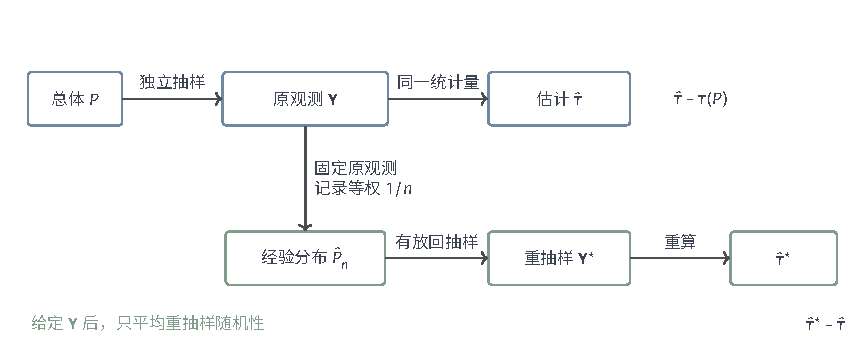
\includegraphics[width=145mm]{figures/00-shared/mathematical-preliminaries-lower/01-random-variables-distributions-and-causality/tikz/statistics-bootstrap-layers/source.pdf}
  \caption{原抽样与条件Bootstrap的两个随机层次。上行从总体\(P\)产生原观测并计算\(\widehat\tau\)，研究其相对\(\tau(P)\)的误差；下行固定同一批原观测，由经验分布\(\widehat P_n\)有放回抽取同样数量的观测，再用同一统计量重算\(\widehat\tau^\ast\)。下行的条件概率只平均重抽样随机性。两类中心化误差的分布能否相互逼近，仍需正文给出的有效性条件。}
  \label{fig:statistics-bootstrap-layers}
\end{figure*}

对独立同分布、方差\(0<\sigma^2<\infty\)的样本均值，这个近似有清楚的缩放口径。
若\(\overline Y^\ast\)由经验分布条件重抽样，则下述条件分布依概率弱收敛：
\[
  \mathcal L\!\left(
    \sqrt n(\overline Y^\ast-\overline Y)\mid\bm Y
  \right)
  \Longrightarrow\mathcal N(0,\sigma^2),
\]
与\(\sqrt n(\overline Y-\mu)\)的极限相同。这里条件分布随原样本而变，本身是随机对象。
具体地，用\(\mathbb E_\ast\)表示给定原数据后的重抽样期望，“依概率弱收敛”指
对每个有界Lipschitz函数\(f\)，
\[
 \mathbb E_\ast f\bigl(\sqrt n(\overline Y^\ast-\overline Y)\bigr)
 \xrightarrow{\mathbb P}\mathbb E f(Z),\qquad Z\sim\mathcal N(0,\sigma^2).
\]
外层的依概率收敛针对原数据的抽样随机性。

此处需要的中心极限定理允许抽样规律随\(n\)改变。
把随机变量逐行排列，第\(n\)行有\(n\)项\(X_{n,1},\ldots,X_{n,n}\)，
这样的排列称为三角阵列（triangular array）。
若每行内的变量独立、中心化，满足
\[
 \sum_{i=1}^n\mathbb E X_{n,i}^2\longrightarrow\sigma^2>0,\qquad
 \sum_{i=1}^n\mathbb E\!\left[
 X_{n,i}^2\mathbb I\{|X_{n,i}|>\varepsilon\}\right]\longrightarrow0
\]
对每个\(\varepsilon>0\)成立，则行和趋于\(\mathcal N(0,\sigma^2)\)。
第二项称为Lindeberg条件，排除了由少数单项主导总波动的情况。
这是所用的独立三角阵列中心极限定理；不要求不同行之间独立，完整证明见概率论教材\scite{math-kallenberg2021probability}。

对给定原数据的重抽样取\(X_{n,i}=(Y_i^\ast-\overline Y)/\sqrt n\)。
行和就是所研究的均值波动；条件均值为零，条件方差和是经验方差。
经验均值等于\(\overline Y\)，经验方差
依概率趋于\(\sigma^2\)，但方差收敛本身还不足以保证条件中心极限定理。有限二阶矩还使
每个\(\varepsilon>0\)对应的条件Lindeberg尾项满足
\[
  \frac1n\sum_{i=1}^n(Y_i-\overline Y)^2
  \mathbb I\{|Y_i-\overline Y|>\varepsilon\sqrt n\}
  \xrightarrow{\mathbb P}0.
\]
这个经验尾项恰好是上述阵列在条件分布下的Lindeberg和。
其收敛可直接由有限二阶矩核对。以趋于一的概率
\(|\overline Y-\mu|\leq\varepsilon\sqrt n/2\)；在此事件上，
若\(|Y_i-\overline Y|>\varepsilon\sqrt n\)，则
\(|Y_i-\mu|>\varepsilon\sqrt n/2\)。又有
\[
 (Y_i-\overline Y)^2\leq2(Y_i-\mu)^2+2(\overline Y-\mu)^2.
\]
因此经验尾项被原中心平方尾的两倍经验平均加\(2(\overline Y-\mu)^2\)控制。
第一项的期望随截断阈值增大而趋零，由Markov不等式依概率趋零；第二项由大数定律趋零。

为把随机条件量接到确定阵列定理，可从任意原数据子列中再抽出一条子子列，
使经验方差和所有正有理\(\varepsilon\)的尾项同时几乎必然收敛；
这是\BookLemmaRef{lem:rv-probability-subsequence}{引理~\ref{lem:rv-probability-subsequence}}的可数对角应用。
尾项关于阈值单调，故该共同满测集上所有正阈值的条件都成立。
逐条固定这样的原数据实现，应用阵列定理便得到条件弱收敛；
再用同一子列判据返回上述测试函数积分的依概率结论。
该结论针对中心化、缩放后的条件分布；它本身不自动证明任意百分位
区间具有高阶准确性。

例~\ref{ex:statistics-running-sensor-calibration}中的经验分布均值为\(10.4\)，经验
方差按分母\(n\)计算恰为\(4\)。因此单次Bootstrap抽样值满足
\[
  \mathbb{E}_\ast[Y^\ast]=10.4,\qquad
  \operatorname{Var}_\ast(Y^\ast)=4,
\]
而二十五次有放回抽样的均值满足
\[
  \operatorname{SE}_\ast(\overline Y^\ast)
  =
  \sqrt{\frac4{25}}=0.4.
\]
若中心化并按标准误标准化后的条件Bootstrap分布可由标准正态分布近似，则正态
Bootstrap区间为
\(10.4\pm1.96\times0.4=[9.62,11.18]\)，与已知方差高斯区间在这个构造例中重合。
重合来自经验方差刚好等于已知噪声方差以及均值的光滑性，不是Bootstrap总会复制参数
区间的保证。

更一般的统计量可以用线性化研究，但须分别控制原抽样与重抽样的余项。即使已经证明
\[
  \widehat\tau-\tau(P)
  =
  \frac1n\sum_{i=1}^n\operatorname{IF}(Y_i;T,P)
  +o_{\mathbb{P}}(n^{-1/2}),
\]
也还需证明条件重抽样展开，例如对某个数据依赖的中心化函数\(\phi_n\)，
\[
 \widehat\tau^\ast-\widehat\tau
 =\frac1n\sum_{i=1}^n\phi_n(Y_i^\ast)+r_n^\ast,\qquad
 \mathbb E_\ast\phi_n(Y_i^\ast)=0.
\]
所需余项条件是：对每个\(\varepsilon>0\)，
\(\mathbb P_\ast(\sqrt n|r_n^\ast|>\varepsilon)\xrightarrow{\mathbb P}0\)；
这就是这里的条件\(o_{\mathbb P_\ast}(n^{-1/2})\)。
若经验影响函数\(\phi_n\)还满足条件中心极限定理，且极限方差与原影响函数一致，
两边缩放后的分布才趋于同一极限。适当的统计泛函光滑性可以帮助建立这些条件，
不能只把原展开中的\(P\)换成\(\widehat P_n\)便认定已证明Bootstrap有效\scite{vanderVaart1998asymptotic}。

一个短反例说明为何必须单独检查重抽样。连续有限方差分布下，取
\[
 \widehat\tau_n=\overline Y+n^{-1/2}
 \mathbb I\{\text{样本中有重复值}\}.
\]
原样本几乎必然没有重复值，所以它具有与均值完全相同的原抽样展开。
但从\(n\)个不同观测有放回抽\(n\)次，全不重复的条件概率为
\(n!/n^n\leq\exp(-(n-1)/2)\)，趋于零；不等式来自
\(\log(1-j/n)\leq-j/n\)的逐项求和。
于是\(\sqrt n(\widehat\tau_n^\ast-\widehat\tau_n)\)额外平移约\(1\)，
没有逼近原统计量的中心化极限。
样本最大值之类统计量
没有这种常规线性展开：经验分布不会生成比当前最大值更大的观测，简单Bootstrap便可能
错误描述尾部。
% Baseline T:1247-1249
重采样单位必须跟独立单位一致。配对实验对整对数据重采样；多个记录属于同一用户时对
用户群组重采样；时间相关数据使用保留局部依赖的块Bootstrap。逐条重采样会把共享噪声
误当作独立波动，通常低估标准误。
\subsubsection{序贯覆盖与可预测设计}
% Baseline S:642-649
重采样解决的是固定程序的误差近似；不断增加样本并反复查看区间，还增加了停止规则的问题。若每次查看都各自给出同一覆盖率，不能推出全部查看同时覆盖。需要把保证改成一个共同事件：真实参数在所有时刻的区间内，这样根据已有数据停止时仍可继承覆盖。
\begin{definition}[置信序列]
  \label{def:stoch-confidence-sequence}
  对参数为\(\theta\)时的数据分布\(\mathbb P_\theta\)，数据依赖集合\((C_t)_{t\geq1}\)若在时刻\(t\)由\(\mathcal F_t\)确定，且对每个允许的\(\theta\)满足
  \[ \mathbb P_\theta(\theta\in C_t\text{ 对所有 }t\geq1)\geq1-\delta, \]
  则称为覆盖水平\(1-\delta\)的\term{置信序列}（confidence sequence），其中\(0<\delta<1\)。
\end{definition}
它在同一个高概率事件上覆盖所有时刻，因而允许根据当前数据决定何时查看或停止。固定$n$的置信区间只承诺
预先指定时刻的覆盖；反复查看直到区间排除某个值，会改变错误概率。
一个可直接计算的标量构造来自Hoeffding界。若\(X_i\in[0,1]\)独立同分布，均值为
\(\mu\)，给第\(n\)次查看分配错误预算
\(\delta_n=\delta/[n(n+1)]\)，则\(\sum_{n\geq1}\delta_n=\delta\)。定义
\[
C_n=\left[\overline X_n-
\sqrt{\frac{\log(2n(n+1)/\delta)}{2n}},
\ \overline X_n+
\sqrt{\frac{\log(2n(n+1)/\delta)}{2n}}\right]\cap[0,1].
\]
对全部时刻的坏事件取并集，即得
\(\mathbb P(\forall n,\mu\in C_n)\geq1-\delta\)。
取\(\delta=0.05,n=100\)，半宽约为\(0.254\)；固定时刻Hoeffding区间半宽约为
\(0.136\)。同时保证付出了更宽范围，这个简单预算构造也不是最紧的边界。条件均值恒为
\(\mu\)且条件范围仍为\([0,1]\)时，条件Hoeffding论证给出同样控制；任意相关观测则不能直接使用。
预先固定有限个候选时，可再将\(\delta\)分给各候选以保证选择后的覆盖。无限搜索或用同一数据重新设计目标，需要额外统一控制或独立评价数据。

对于可预测的向量设计，下面回用\BookSectionRef{sec:rv-anytime}{第~\ref{sec:rv-anytime}节}的自归一化界，把累计噪声转成参数置信椭球。
% Baseline S:816-924
取$\bm{V}_0=\lambda\bm{I}$，$\lambda>0$，并定义岭回归估计
\begin{equation}
  \widehat{\bm{\theta}}_t
  =\bm{V}_t^{-1}\sum_{s=1}^{t}\bm{x}_s y_s.
  \label{eq:stoch-ridge-estimator}
\end{equation}
由\BookEquationRef{eq:stoch-adaptive-linear-observation}{式~\eqref{eq:stoch-adaptive-linear-observation}}，
\[
  \bm{V}_t
  (\widehat{\bm{\theta}}_t-\bm{\theta}^{\star})
  =
  \bm{S}_t-\lambda\bm{\theta}^{\star}.
  \]
若还知道$\lVert\bm{\theta}^{\star}\rVert_2\leq B$，三角不等式给出
\begin{align}
  \lVert
    \widehat{\bm{\theta}}_t-\bm{\theta}^{\star}
  \rVert_{\bm{V}_t}
  &\leq
  \lVert\bm{S}_t\rVert_{\bm{V}_t^{-1}}
  +
  \lambda
  \lVert\bm{\theta}^{\star}\rVert_{\bm{V}_t^{-1}}
  \notag\\
  &\leq
  R\sqrt{
    2\log\left(
      \frac{\det(\bm{V}_t)^{1/2}}
           {\lambda^{d/2}\delta}
    \right)
  }
  +\sqrt{\lambda}B
  =:\beta_t(\delta).
  \label{eq:stoch-adaptive-confidence-ellipsoid}
\end{align}
第二个不等式使用$\bm{V}_t\succeq\lambda\bm{I}$。因此
\[
  \mathcal{C}_t(\delta)
  =
  \left\{
    \bm{\theta}:
    \lVert\bm{\theta}-\widehat{\bm{\theta}}_t
    \rVert_{\bm{V}_t}
    \leq\beta_t(\delta)
  \right\}
\]
在同一个概率至少为$1-\delta$的事件上，对所有$t$都包含真实参数。这是置信椭球而不是
欧氏球：观测充分的方向较窄，信息不足的方向较宽。

\begin{example}[二维自适应查询]
  \label{ex:stoch-two-dimensional-adaptive-design}
  设$d=2$、$\lambda=1$，每次只能在
  $\bm{e}_1=(1,0)^\top$与$\bm{e}_2=(0,1)^\top$中选择一个观测方向。算法在第
  $t$步根据上一轮椭球在两个方向上的宽度调整查询概率，再抽取方向：所用随机数在给定此前历史后服从\(\operatorname{Unif}(0,1)\)，并与当前噪声条件独立，且在噪声出现前完成抽取。较宽的方向获得较大概率，但不必每次选中；把这次抽取纳入观测前的信息后，$\bm{x}_t$可预测，噪声的条件次高斯界也保持。

  若前四次选择中$\bm{e}_1$出现三次、$\bm{e}_2$出现一次，则
  \[
    \bm{V}_4
    =
    \begin{pmatrix}
      4&0\\
      0&2
    \end{pmatrix},
    \qquad
    \det(\bm{V}_4)=8.
  \]
  对任意方向$\bm{x}$，椭球给出的预测误差满足
  \[
    |\langle
      \bm{x},
      \widehat{\bm{\theta}}_4-\bm{\theta}^{\star}
    \rangle|
    \leq
    \beta_4(\delta)
    \lVert\bm{x}\rVert_{\bm{V}_4^{-1}}.
  \]
  因而两个坐标方向的半宽分别与$1/2$和$1/\sqrt2$成比例。第一个方向访问更多，区间
  更窄；下一次提高第二个方向的查询概率，是由已有信息决定的自适应设计。定理仍然适用，因为它在每次
  新噪声产生之前固定当前方向，并在一个事件上同时控制全部时刻。
\end{example}

图~\ref{fig:stochastic-design-ellipsoids}还比较了相同四次预算在两个方向各访问两次的情形：此时\(\bm V_4=\operatorname{diag}(3,3)\)。均衡访问扩大第一个方向的几何半宽，却缩小第二个方向的半宽；因此设计会改变误差的方向分配，不能只比较一个总访问数。图中把两条二次型的右侧统一设为\(1\)，仅比较几何；真正的置信椭球还要分别乘上各自的\(\beta_4(\delta)\)，其行列式项也会改变。

\begin{figure}[htbp]
  \centering
  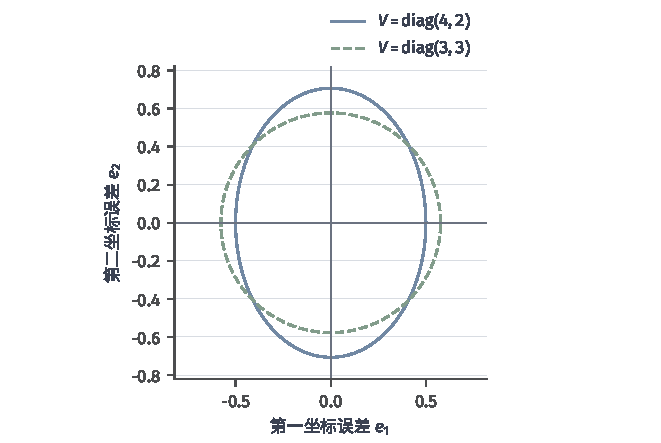
\includegraphics[width=\linewidth]{figures/00-shared/mathematical-preliminaries-lower/01-random-variables-distributions-and-causality/matplotlib/stochastic-design-ellipsoids/figure.pdf}
  \caption{二维设计的归一化误差几何（解析式教学图）。蓝实线为\(\bm e^\top\operatorname{diag}(4,2)\bm e=1\)，绿虚线为\(\bm e^\top\operatorname{diag}(3,3)\bm e=1\)。它们不是已经具有相同覆盖概率的数值置信区间；真实置信半径由式~\eqref{eq:stoch-adaptive-confidence-ellipsoid}另行确定。}
  \label{fig:stochastic-design-ellipsoids}
\end{figure}

这个例子也说明为什么不能把独立样本界中的$n$换成某个动作的访问次数。参数误差是向量，
不同特征方向可能相关；置信宽度由$\bm{x}^{\top}\bm{V}_t^{-1}\bm{x}$决定，而不是只由
某个坐标被访问多少次决定。行列式项又要为算法可能探索的全部方向支付复杂度。

\paragraph{可预测设计与数据依赖的边界}
自归一化界允许$\bm{x}_t$依赖$\mathcal{F}_{t-1}$，不允许它依赖当前$\eta_t$后再伪装成
预先选择。若传感器先看到当前噪声再决定是否记录，$\bm{x}_t\eta_t$的条件平均可能不再为
零，指数超鞅的第一步就会失败。类似地，模型失配使
$\mathbb{E}[y_t\mid\mathcal{F}_{t-1},\bm{x}_t]$不等于
$\langle\bm{x}_t,\bm{\theta}^{\star}\rangle$时，估计误差中会增加系统偏差，原半径没有证明能控制这项偏差，
不能继续给出同一个真实参数的原覆盖保证。

条件次高斯性也不是有限方差的同义词。重尾噪声可能需要截断、稳健均值或只使用有限矩的
其他序贯工具；直接套用\BookEquationRef{eq:stoch-vector-self-normalized-bound}{式~\eqref{eq:stoch-vector-self-normalized-bound}}会低估尾部。
$\lambda$保证初期矩阵可逆并编码参数范数先验，但过大的$\lambda$会增加
$\sqrt{\lambda}B$偏差项。置信椭球控制统计误差，不保证选择策略会访问所有对任务重要的
方向；探索是否充分仍要由设计规则与任务目标另行证明。

\subsection{假设检验的错误控制}
\subsubsection{检验目标、证据与功效}
\label{sec:statistics-testing-errors}
\label{sec:statistics-selection-multiplicity}
% Baseline T:1012-1164
区间描述目标的可能范围，\term{假设检验}（hypothesis testing）则检查数据与一个
命题是否相容。
一个确定性规则对每组记录只作拒绝或不拒绝两种选择。但在离散观测中，直接增加一整个拒绝事件可能使误拒概率超过预算；允许在边界记录上再随机拒绝，可以细调这项概率。于是用取值于\([0,1]\)的函数统一表示拒绝概率，确定性规则对应只取\(0,1\)的特例。
\begin{definition}[随机化检验函数]
  \label{def:statistics-randomized-test-function}
  若单个观测的可测空间为\(\mathcal{Y}\)，则
  \term{随机化检验函数}（randomized test function）是可测映射
  \[
    \varphi:\mathcal{Y}^n\to[0,1].
  \]
  观察到\(\bm{Y}=\bm{y}\)后，检验以概率\(\varphi(\bm{y})\)拒绝原假设。等价地，可另取
  独立的\(U\sim\operatorname{Unif}(0,1)\)，并在
  \(U\leq\varphi(\bm{y})\)时拒绝。只取\(0,1\)值的检验是非随机化特例，其拒绝域为
  \(R=\{\bm{y}:\varphi(\bm{y})=1\}\)。
\end{definition}

原假设\(H_0\)指定被控制误报的情形。检验的大小与参数\(\theta\)下的功效分别为
\[
  \sup_{\theta\in H_0}\mathbb{E}_\theta[\varphi(\bm Y)],
  \qquad
  \mathbb{E}_\theta[\varphi(\bm Y)].
\]
水平为\(\alpha\)要求
\[
  \sup_{\theta\in H_0}
  \mathbb{E}_\theta[\varphi(\bm Y)]
  \leq\alpha.
\]
在\(H_0\)为真时拒绝是第一类错误；在备择\(H_1\)为真时不拒绝是第二类错误。
对非随机化检验，这些期望分别退化为拒绝域概率。效应量描述差异有多大，样本量则影响
能否把该差异从噪声中区分出来。

\term{\(p\)值}（\(p\)-value）的一种常见构造，是在原假设下计算至少与当前统计量同样极端结果的概率。复合假设或其他构造还需满足下面的有效性要求。
\begin{definition}[有效p值]
  \label{def:statistics-valid-p-value}
  一个取值于\([0,1]\)的可测统计量\(p(\bm Y)\)是复合原假设\(H_0\)下的有效\(p\)值，若对每个
\(u\in[0,1]\)都有
\[
  \sup_{\theta\in H_0}\mathbb{P}_\theta\{p(\bm Y)\leq u\}\leq u.
\]
\end{definition}
这项零假设下的超均匀性质才保证按阈值\(\alpha\)拒绝时控制第一类错误。观察到的
\(p\)值不是原假设为真的概率，也不是效应量。仍取已知\(\sigma\)的高斯位置模型，
检验\(H_0:\theta=0\)时
\[
  Z=\frac{\sqrt n\,\overline Y}{\sigma},\qquad
  p=2\{1-\Phi(|Z|)\}.
\]
若\(\theta=\delta\)，双侧检验功效为
\[
  \mathbb{P}_\delta(|Z|>z_{1-\alpha/2})
  =
  1-\Phi\left(z_{1-\alpha/2}-\frac{\sqrt n\delta}{\sigma}\right)
  +\Phi\left(-z_{1-\alpha/2}-\frac{\sqrt n\delta}{\sigma}\right).
\]
小样本下“不显著”可能只表示功效不足。保持观测到的\(|\overline Y|>0\)及\(\sigma>0\)不变时，增大\(n\)会使上式的\(p\)值变小；固定真实效应的另一次抽样却不保证\(p\)值逐次减小。

检验族还可反演为置信集合。对每个候选值\(\theta_0\)，设
\(\varphi_{\theta_0}(\bm Y)\in\{0,1\}\)是水平不超过\(\alpha\)的检验，并定义
\[
  C(\bm Y)=\{\theta_0:\varphi_{\theta_0}(\bm Y)=0\}.
\]
当真实值为\(\theta\)时，
\[
  \mathbb{P}_\theta\{\theta\notin C(\bm Y)\}
  =\mathbb{P}_\theta\{\varphi_\theta(\bm Y)=1\}\leq\alpha,
\]
所以\(C\)具有至少\(1-\alpha\)覆盖率。这里必须对同一模型、同一尾部规则和同一
标准误反演；选择后换检验或只挑有利方向会破坏证明。

\begin{example}[同一效应量下的证据与功效]
\label{ex:statistics-evidence-power-same-effect}
设噪声标准差已知为\(\sigma=2\)，观测均值为\(\overline y=1\)，检验
\(H_0:\theta=0\)。当\(n=4\)时，\(Z=1\)，双侧\(p\)值约为\(0.317\)；
当\(n=100\)时，\(Z=5\)，双侧\(p\)值小于\(10^{-6}\)。两次实验报告的标准化
效应\(\overline y/\sigma=0.5\)相同，证据强度却因标准误不同而变化。

若真实值确为\(\delta=1\)，显著性水平为\(0.05\)，则\(n=4\)时双侧检验功效约为
\[
  1-\Phi(1.96-1)+\Phi(-1.96-1)\approx0.17.
\]
此时未拒绝原假设并不支持“差异为零”。若实际问题把绝对差异不超过\(0.2\)视为等效，
还需要针对\(\Delta=0.2\)设计等效检验；当前样本对这个更严格目标几乎没有辨识力。
\end{example}

\paragraph{似然比排序与Neyman–Pearson引理}
固定允许的误拒概率后，希望尽量提高识别另一个指定规律的概率。对同一份记录，若它在备择规律下比在原假设下更常见，就应优先把它放入拒绝域；似然比给出这个相对证据的排序，阈值再用完允许的错误预算。
下面的经典引理给出两个简单假设之间的最强检验\scite{math-lehmann2005testing}。
\begin{theorem}[Neyman--Pearson引理]
\label{thm:statistics-neyman-pearson}
取\(0<\alpha<1\)。对两个完全指定的简单假设\(H_0:P=P_0\)与\(H_1:P=P_1\)，设
\(P_1\ll P_0\)，似然比为\(\Lambda=\mathrm dP_1/\mathrm dP_0\)。在所有大小
不超过\(\alpha\)的检验中，拒绝大似然比并在边界适当随机化的检验具有最大功效。
\end{theorem}

\begin{proof}
取常数\(c\geq0\)与边界随机化概率，使检验\(\varphi^\star\)满足
\(\mathbb{E}_0[\varphi^\star]=\alpha\)，并在\(\Lambda>c\)时拒绝、在
\(\Lambda<c\)时接受。对任意\(\mathbb{E}_0[\varphi]\leq\alpha\)的检验，
\[
  (\varphi^\star-\varphi)(\Lambda-c)\geq0
\]
逐点成立，因为\(\varphi^\star\)在\(\Lambda>c\)处取最大允许值，在
\(\Lambda<c\)处取最小允许值。对\(P_0\)积分得到
\[
  \mathbb{E}_1[\varphi^\star-\varphi]
  \geq c\,\mathbb{E}_0[\varphi^\star-\varphi]\geq0.
\]
所以\(\varphi^\star\)的备择拒绝概率不小于任何同大小检验。
\end{proof}

这个结论只直接覆盖两个简单假设。复合假设需要处理未知参数，不一定存在一致最强检验。
在隐私攻击审计中，\(P_0\)与\(P_1\)可分别表示目标记录不在与在训练集时的输出分布；
似然比给出理想攻击排序，但实际审计还要估计这两个分布并计入选择偏差。

\subsubsection{分类观测与随机化检验}
两个分类变量的列联表中，原假设为独立时，期望格数是
\[
  E_{r,c}=\frac{N_{r,\cdot}N_{\cdot,c}}{N},\qquad
  X^2=\sum_{r,c}\frac{(N_{r,c}-E_{r,c})^2}{E_{r,c}}.
\]
计算时先删去零边际计数的行列，保证保留格子的\(E_{r,c}>0\)。当样本独立同分布、类别数\(R,C\)固定，且原假设下各格子的总体概率为正时，随\(N\to\infty\)，
\(X^2\)的分布趋于自由度\((R-1)(C-1)\)的卡方分布。稀疏格数会破坏近似，可合并有
科学意义的类别或使用精确、置换方法。条件独立检验还要控制第三个变量；把样本简单切成
大量小层会带来新的稀疏性，不能由普通卡方检验自动解决。

差异检验把“无差异”放在原假设中。等效性检验先给出有实际含义的可接受差异界
\(\Delta>0\)。记\(\delta=\theta_A-\theta_B\)，两个单侧检验（two one-sided
tests, TOST）把不等效原假设写成两个集合的并：
\[
  H_0=H_{0,L}\cup H_{0,U},
  \qquad
  H_{0,L}:\delta\leq-\Delta,
  \qquad
  H_{0,U}:\delta\geq\Delta.
\]
对应备择为\(-\Delta<\delta<\Delta\)。TOST只有在水平\(\alpha\)的下侧检验拒绝
\(H_{0,L}\)，并且水平\(\alpha\)的上侧检验也拒绝\(H_{0,U}\)时，才拒绝总体原假设。
取\(0<\alpha<1/2\)。例如，若\(\widehat\delta\)的标准误为\(s>0\)，且标准化统计量服从相应正态近似，
拒绝条件为
\begin{equation}
  \frac{\widehat\delta+\Delta}{s}>z_{1-\alpha}
  \quad\text{且}\quad
  \frac{\widehat\delta-\Delta}{s}<z_{\alpha}.
  \label{eq:statistics-tost-rejection}
\end{equation}
这等价于把双侧\(1-2\alpha\)置信区间完整放入
\((-\Delta,\Delta)\)。总体第一类错误并非\(2\alpha\)：只要
\(\delta\in H_0\)，至少有一个单侧原假设为真，而总体拒绝事件包含在拒绝这个真原假设
的事件中，所以其概率至多为\(\alpha\)。非劣效检验只排除一个方向，例如
\(H_0:\delta\leq-\Delta\)。未拒绝差异检验的零假设不等于证明等效。
图~\ref{fig:statistics-difference-equivalence}把这两个判据放在同一个差异轴上。蓝色区间检查零点是否被排除，绿色区间检查它是否完整位于预先规定的等效界内。第一行的区间太宽，既不能排除零，也不能排除具有实际意义的差异；第二行围绕零且足够窄，可以支持等效。第三行的差异虽已足以排除零，其范围仍完整位于等效界内，因此“统计上非零”与“在指定尺度下等效”可以同时成立。两个检验回答的问题不同，不能仅用是否显著替代实际差异范围的判断。

\begin{figure}[htbp]
  \centering
  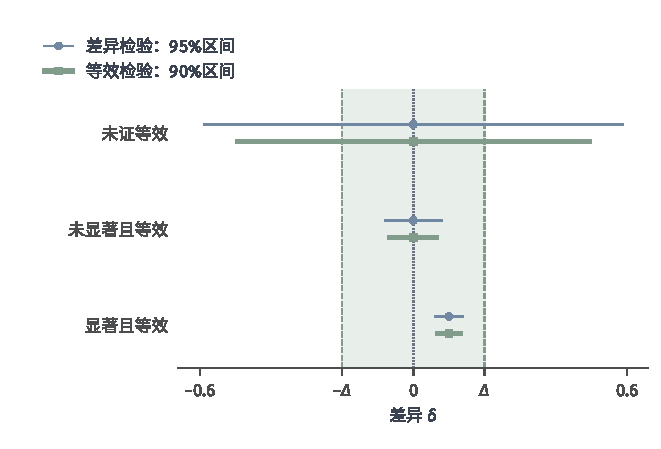
\includegraphics[width=112mm]{figures/00-shared/mathematical-preliminaries-lower/01-random-variables-distributions-and-causality/matplotlib/statistics-difference-equivalence/figure.pdf}
  \caption{差异检验与等效检验的区间判读。教学设定为已知标准误的正态差异估计，\(\alpha=0.05\)、\(\Delta=0.2\)；三行\((\widehat\delta,s)\)依次为\((0,0.30)\)、\((0,0.04)\)、\((0.10,0.02)\)。蓝细线为差异检验对应的\(95\%\)区间，绿粗线为TOST对应的\(90\%\)区间，浅绿带表示\((-\Delta,\Delta)\)。第三行同时排除零并支持等效；两类区间使用不同覆盖水平，不能互换。}
  \label{fig:statistics-difference-equivalence}
\end{figure}

% Baseline T:1232-1245
\term{置换检验}（permutation test）近似的不是估计量抽样分布，而是零假设下标签可
交换时的随机化分布。两组观测在“处理标签不影响联合分布”的原假设下，可反复打乱标签
并重算组间差异。若分配机制只允许在区组内交换，就必须在区组内置换；任意全局打乱会
制造实验中不可能出现的分配。

设允许的置换构成一个含\(M\)个元素的有限群，原假设下观测联合分布在该群作用下不变。把观测统计量与全部群置换统计量一起排序；没有并列时，群对称性使秩具有均匀规律，存在并列时使用
\[
  p_{\mathrm{perm}}
  =\frac{\#\{\text{置换统计量不小于观测值}\}}{M}
\]
得到超均匀而可能保守的\(p\)值。若独立、均匀地从该群抽取\(B\)个置换，常用
\((1+\#\{\text{抽样置换不小于观测值}\})/(B+1)\)保留有限模拟下的保守性。
仅有两组均值相等并不保证整批标签可交换；交换性必须来自更强的零假设或随机分配设计。
\subsubsection{多重比较与序贯查看的错误控制}
% Baseline T:1256-1293
单个检验的第一类错误为\(\alpha\)，不代表同时尝试许多候选后仍只有
\(\alpha\)的误报概率。若\(m\)个原假设都为真，联合界给出
\[
  \mathbb{P}(\text{至少一次误拒绝})
  \leq\sum_{j=1}^m\mathbb{P}(\text{拒绝 }H_j)
  \leq m\alpha.
\]
Bonferroni方法把每项阈值设为\(\alpha/m\)，从而控制
\term{族错误率}（family-wise error rate, FWER）。它不要求检验独立，但候选很多时
可能保守。

Holm方法把\(p\)值从小到大排序，并依次将
\(p_{(j)}\)与\(\alpha/(m-j+1)\)比较，遇到第一个未拒绝项即停止。若第一个被错误
拒绝的真原假设位于位置\(j\)，设真原假设总数为\(m_0\)，则前\(j-1\)项均为假
原假设，所以\(m-j+1\geq m_0\)。该真原假设的\(p\)值因而不超过
\(\alpha/(m-j+1)\leq\alpha/m_0\)。对全部\(m_0\)个真原假设应用联合界，便把
发生任一错误拒绝的概率控制在\(\alpha\)以内。它与Bonferroni一样不要求独立，但利用
了逐步比较。

当目标是控制所有拒绝中错误发现的期望比例时，可使用
\term{错误发现率}（false discovery rate, FDR）。设\(R\)为拒绝的总数、\(V\)为其中
被错误拒绝的真原假设数，则
\[
  \operatorname{FDR}=\mathbb E\left[\frac{V}{\max(R,1)}\right].
\]
当\(R=0\)时，错误发现比例约定为零；这是随机比例的期望，不是
\(\mathbb EV/\mathbb ER\)。Benjamini--Hochberg过程将
\(p\)值排序为\(p_{(1)}\leq\cdots\leq p_{(m)}\)，找最大
\[
  k=\max\left\{j:p_{(j)}\leq\frac{j}{m}q\right\},
\]
并拒绝前\(k\)项；若集合为空，则取\(k=0\)，不拒绝任何假设。若全部\(p\)值相互
独立，且每个真原假设下的\(p\)值满足
\(\mathbb P(p_j\leq u)\leq u\)（\(0\leq u\leq1\)），该过程控制FDR不超过目标
\(q\in(0,1)\)\scite{statistics-benjamini-hochberg1995}。扩展到依赖检验需要更精确的联合分布条件，不能仅凭两两正相关或任意
依赖就沿用这项保证。

从多个模型中挑选测试误差最小者，再把该最小值当成固定模型的无偏评估，通常会引入选择后的乐观偏差。
% Baseline T:1330-1343
持续查看同一数据也构成选择。固定时刻满足
\(\mathbb{P}(p_t\leq\alpha)\leq\alpha\)并不推出
\(\mathbb{P}(\exists t:p_t\leq\alpha)\leq\alpha\)。预先规定查看次数可分配
\(\alpha\)预算；更灵活的停止规则需要序贯检验、置信序列或对整个证据过程的控制。
停止规则属于推断程序的一部分，不能在看到结果后删去。

一种单次证据是\(e\)值（e-value）：非负统计量\(E\)若在每个零假设分布\(P\)下
满足\(\mathbb E_PE\leq1\)，就称为有效\(e\)值。由Markov不等式，
\(P(E\geq1/\alpha)\leq\alpha\)，所以大值可以用来拒绝零假设。
但逐个固定时刻的\(E_t\)都是有效\(e\)值，仍不足以保证可以任意停止；
下文用非负超鞅给出一种能同时控制所有时刻的证据过程。

定义~\ref{def:stoch-confidence-sequence}的\term{置信序列}（confidence sequence）把所有时刻的覆盖放在同一个高概率事件中。这比每个固定时刻各自覆盖更强，因为允许依据当前数据决定何时停止查看。
若\((E_t)\)在原假设下是从\(E_0=1\)开始的非负超鞅，则Ville不等式给出
\[
  \mathbb{P}_0\left\{\sup_{t\geq0}E_t\geq\frac1\alpha\right\}\leq\alpha.
\]
因此可以在任意由过去信息决定的停止时刻按阈值查看\(E_t\)，而不增加这项越界概率。
这不表示停止后的点估计无偏，也不表示同时尝试多个证据过程无需额外控制；覆盖、估计
偏差和模型选择证据仍是不同问题。

\section{有限观测下的推断下界}
\label{sec:information-lower-bounds}

若两套候选规律产生很相近的观测分布，却对应相距较远的目标值，那么程序很难从记录辨认目标属于哪套规律。前面的分布差异现在成为辨认难度的依据。我们固定候选总体、目标及可用观测，对所有估计程序的错误给出下界；这个下界来自信息不足，不依赖某个特定算法的实现。

\subsection{固定观测下的分布区分}
\label{sec:information-fixed-observations}

先把整批观测的分布视为已给定，不让程序根据中途结果改变取样位置。
两候选比较利用TV，多候选比较则需要把候选数量也纳入信息预算。

\subsubsection{两个候选的区分下界}
\label{sec:information-two-candidates}

设观测\(Z\)来自\(P_0\)或\(P_1\)，先验各为\(1/2\)。
检验\(\psi(Z)\in\{0,1\}\)以事件\(A=\{\psi=1\}\)选择第二个候选，则错误和为
\[
  P_0(A)+P_1(A^{\mathsf c})=1-\{P_1(A)-P_0(A)\}.
\]
取使密度差为正的事件达到上确界，得到
\begin{equation}
  \inf_\psi\{P_0(\psi=1)+P_1(\psi=0)\}
     =1-d_{\mathrm{TV}}(P_0,P_1).
  \label{eq:information-binary-testing-tv}
\end{equation}
随机化检验只是把指标改为\([0,1]\)值函数，按TV的函数表达也不能降低这个值。
在等先验下，最小总体错误是右侧的一半；两类条件错误之和本身不是总体错误。

上面界定的是“判断观测来自哪个候选”的最优错误率。实际问题常是估计一个数值（比如均值），它与检验有什么关系？直觉是：如果一个估计量真的足够准，那么面对两个相隔足够远的候选目标，它的估计值必然更靠近真实的那一个，于是可以直接用“估计值离谁更近”构造一个检验。这说明数值估计的精度不可能高于二选一检验所能达到的分辨力——据此可以把刚得到的检验下界翻译成任意估计量的误差下界。

\begin{theorem}[Le Cam两点下界]
\label{thm:information-le-cam}
设观测模型\(P_0,P_1\)对应目标\(\theta_0,\theta_1\)，
在目标空间度量\(d\)下有\(d(\theta_0,\theta_1)\geq2s\)，\(s>0\)。
任意估计量\(\widehat\theta\)均满足
\begin{equation}
  \max_{j\in\{0,1\}}P_j\{d(\widehat\theta,\theta_j)\geq s\}
  \geq\frac{1-d_{\mathrm{TV}}(P_0,P_1)}2.
  \label{eq:information-le-cam}
\end{equation}
\end{theorem}
\begin{proof}
构造最近目标检验
\(\psi=\mathbb I\{d(\widehat\theta,\theta_1)<d(\widehat\theta,\theta_0)\}\)，
距离相等时选\(0\)。若真实为\(0\)且估计误差小于\(s\)，由三角不等式，
估计与\(\theta_1\)的距离大于\(s\)，检验不会错。
真实为\(1\)时同理。因此检验错误分别包含在估计坏事件内。
两个坏事件概率之和至少为\(1-d_{\mathrm{TV}}(P_0,P_1)\)，
其中最大者至少为一半，即得结论。
\end{proof}

若每个候选下都得到\(n\)个独立同分布观测，联合密度比是单次密度比的乘积，
取对数并平均得到
\(D_{\mathrm{KL}}(P_0^{\otimes n}\Vert P_1^{\otimes n})
=nD_{\mathrm{KL}}(P_0\Vert P_1)\)。
取单次规律为\(\mathcal N(-a,\sigma^2)\)与\(\mathcal N(a,\sigma^2)\)，
目标均值相距\(2a\)，整批KL为\(2na^2/\sigma^2\)。
令\(a=\sigma/(2\sqrt n)\)，KL为\(1/2\)，Pinsker给出TV至多\(1/2\)。
所以任何均值估计量都至少在一个候选下，以不小于\(1/4\)的概率产生
不小于\(\sigma/(2\sqrt n)\)的绝对误差。
若评价平方误差，还可由这个事件下界得到最坏风险至少\(\sigma^2/(16n)\)。
这些常数来自所选两点及放缩，不声称最优。

图~\ref{fig:information-le-cam-estimation-testing}把观测的可区分程度与目标的估计精度放在两个面板中。对这一高斯例，整批观测的对数似然比为
\[
 \log\frac{\mathrm dP_1^{\otimes n}}{\mathrm dP_0^{\otimes n}}
 =\frac{2a}{\sigma^2}\sum_{i=1}^nX_i
 =\frac{2an}{\sigma^2}\overline X,
\]
所以最优等先验检验按样本均值的正负选择候选。左图两条密度仍有重叠，这部分概率限制了检验的准确程度；右图两个半径为\(a\)的开误差区间互不相交，说明估计值一旦落在真实目标的小误差区间内，最近目标检验就不会错。两点下界同时使用了这两件事：观测不易区分，而小估计误差又必须足以区分目标。

\begin{figure*}[htbp]
  \centering
  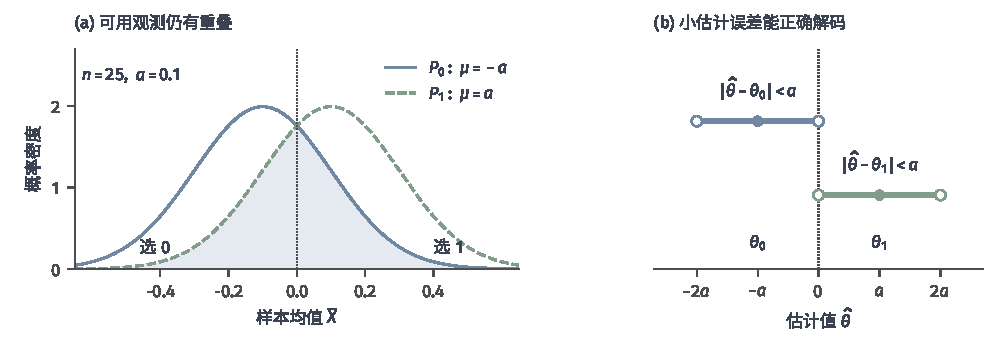
\includegraphics[width=169mm]{figures/00-shared/mathematical-preliminaries-lower/01-random-variables-distributions-and-causality/matplotlib/information-le-cam-estimation-testing/figure.pdf}
  \caption{由估计精度连接到二选一检验的高斯教学例。取\(\sigma=1,n=25,a=0.1\)，左图样本均值在两候选下分别服从\(\mathcal N(-a,0.2^2)\)与\(\mathcal N(a,0.2^2)\)；浅蓝阴影是两密度逐点较小值之下的面积，等于\(1-d_{\mathrm{TV}}\)，其一半约为\(0.3085\)，是最小等先验总体错误。右图的实点为目标，空心端点不属于对应的开误差区间；两个区间只在边界处相接。正文的\(1/4\)是经Pinsker放缩得到的下界，并非左图的精确最小错误。}
  \label{fig:information-le-cam-estimation-testing}
\end{figure*}

\subsubsection{多个候选的区分下界}
\label{sec:information-many-candidates}

两点只要求区分一个二元选择；高维问题可能同时包含许多不同目标。
令\(V\)在\(\{1,\ldots,M\}\)上均匀，给定\(V=v\)后观测\(Z\sim P_v\)。
解码器\(\widehat V(Z)\)的错误概率记为\(p_{\mathrm e}\)。
即使\(Z\)连续，\(V\)的条件熵仍可按其有限后验概率求熵，再对\(Z\)积分。

\begin{theorem}[Fano不等式]
\label{thm:information-fano}
对\(M\geq2\)及上述观测模型，
\begin{equation}
  p_{\mathrm e}\geq1-\frac{I(V;Z)+\log2}{\log M}.
  \label{eq:information-fano}
\end{equation}
\end{theorem}
\begin{proof}
令\(E=\mathbb I\{\widehat V\neq V\}\)。给定\(Z\)且\(E=0\)时，
\(V=\widehat V(Z)\)已确定；给定\(E=1\)时，至多还有\(M-1\)个可能索引。
有限字母表上最大熵为均匀熵，这也可由与均匀分布的Gibbs不等式得到。
于是
\[
\begin{aligned}
  H(V\mid Z)
  &\leq H(V,E\mid Z)\\
  &=H(E\mid Z)+H(V\mid E,Z)\\
  &\leq\log2+p_{\mathrm e}\log(M-1)
   \leq\log2+p_{\mathrm e}\log M.
\end{aligned}
\]
又因\(H(V)=\log M\)，互信息分解给出
\(H(V\mid Z)=\log M-I(V;Z)\)。移项得到结论。
随机化解码可把独立随机种子并入\(Z\)，不会增加关于\(V\)的信息。
\end{proof}

若目标集合中有两两距离至少\(2s\)的有限分离集
\(\{\theta_1,\ldots,\theta_M\}\)，误差小于\(s\)就能最近邻解码。
这把前面计数与打包的工具接到统计下界：候选多能提高\(\log M\)，
但必须同时控制观测中含有多少索引信息\scite{math-cover2006information}
令\(\overline P=M^{-1}\sum_uP_u\)，则
\[
  I(V;Z)=\frac1M\sum_vD_{\mathrm{KL}}(P_v\Vert\overline P)
  \leq\frac1{M^2}\sum_{v,u}D_{\mathrm{KL}}(P_v\Vert P_u).
\]
等式来自给定\(V\)的条件KL分解；不等式来自
\(-\log(M^{-1}\sum_u p_u)\leq M^{-1}\sum_u(-\log p_u)\)。
因此
\(\max_vP_v\{d(\widehat\theta,\theta_v)\geq s\}\)
至少为Fano右侧，若右侧为负则只得到平凡下界零。

保留一个可复算的四候选构造：均值为\(\{-3a,-a,a,3a\}\)，
每个候选产生\(n\)个方差\(\sigma^2\)的独立高斯观测。
最小间距为\(2a\)，有序候选对的平均平方距离为\(10a^2\)，故
\[
  I(V;Z)\leq\frac{5na^2}{\sigma^2}.
\]
取\(a=\sigma/(4\sqrt n)\)时右侧为\(5/16\)，Fano给出
\(p_{\mathrm e}\geq1-(5/16+\log2)/\log4\approx0.2746\)。
任意估计器因此至少在一个候选上以这一概率产生不小于\(a\)的误差。
目标分离与观测接近必须同时成立；只罗列许多模型不构成下界证明。

\subsection{序贯观测下的分布区分}
\label{sec:information-sequential-observations}

若观测位置根据已获得的结果改变，最终资料的联合分布也随算法改变。
仍可使用前面的检验不等式，但比较对象应当是包含行动与结果的完整轨迹。

\subsubsection{重复与时序观测的信息累积}
\label{sec:information-sequential-accumulation}

独立重复是简单情形。固定有限个分量\(t=1,\ldots,T\)，假设\(P_t\ll Q_t\)，密度比为\(L_t\)。
乘积规律的比值为\(\prod_tL_t\)，因此
\[
\begin{aligned}
  D_{\mathrm{KL}}\left(\bigotimes_tP_t\Big\Vert\bigotimes_tQ_t\right)
     &=\sum_tD_{\mathrm{KL}}(P_t\Vert Q_t),\\
  D_\alpha\left(\bigotimes_tP_t\Big\Vert\bigotimes_tQ_t\right)
     &=\sum_tD_\alpha(P_t\Vert Q_t),\qquad\alpha>1.
\end{aligned}
\]
第一式由对数把乘积化为和；第二式由独立性使
\(\mathbb E_{\otimes Q_t}\prod_tL_t^\alpha=\prod_t\mathbb E_{Q_t}L_t^\alpha\)。
公式可按扩展值理解，不通过相减处理无限项。

一般序列不独立。设\(Z_{0:T}\)在标准Borel空间取值，两个规律分解为初始分布及
历史条件核，\(P_0\ll Q_0\)，且在相关的\(P\)-历史上
\(P_t(\cdot\mid Z_{<t})\ll Q_t(\cdot\mid Z_{<t})\)。
\BookChapterRef{chap:random-sequences-and-processes}{第~\ref{chap:random-sequences-and-processes}章}的轨迹换测度给出联合密度比
\[
  L_{0:T}=L_0(Z_0)\prod_{t=1}^T L_t(Z_t\mid Z_{<t}).
\]
对数相加，再对每一项先按历史条件平均，得到
\begin{equation}
\begin{aligned}
 D_{\mathrm{KL}}(P_{0:T}\Vert Q_{0:T})
 &=D_{\mathrm{KL}}(P_0\Vert Q_0)\\
 &\quad+\sum_{t=1}^T\mathbb E_{Z_{<t}\sim P}
 D_{\mathrm{KL}}\bigl(P_t(\cdot\mid Z_{<t})
                     \Vert Q_t(\cdot\mid Z_{<t})\bigr).
\end{aligned}
\label{eq:information-trajectory-kl-chain}
\end{equation}
这是式~\eqref{eq:information-kl-conditional-chain}的反复应用。
有限时域中每个条件对数比的负部积分均有统一有限界，
故可合法按扩展值累加；得到有限数值则还需累计条件KL有限。
期望必须沿前向分布\(P\)实际产生的历史计算。

轨迹包含行动时，同一算法在同一历史上使用相同的条件行动核，
所以比较两个环境时行动因子相消；两个环境的历史频率却不会相消。
在同一环境比较两条策略时，则是环境核相消，剩下条件行动KL。
若两者都改变，不能省略其中任何一组项。

Rényi不能把条件散度直接按\(P\)平均。一个充分组合条件是：在\(Q\)-几乎处处的历史上，
\(P_t(\cdot\mid h_{<t})\ll Q_t(\cdot\mid h_{<t})\)，并且有确定的统一界
\[
  D_\alpha(P_t(\cdot\mid h_{<t})\Vert Q_t(\cdot\mid h_{<t}))
  \leq\varepsilon_t.
\]
为简化记号从\(t=1\)开始且初始历史固定。在\(Q\)下从最后一步取条件期望，
\[
  \mathbb E_Q[L_t^\alpha\mid h_{<t}]
       \leq e^{(\alpha-1)\varepsilon_t}.
\]
前面的密度比是历史可测量，因此每消去一步至多乘上这个常数。
反复迭代后
\[
  \mathbb E_Q L_{1:T}^{\alpha}
  \leq e^{(\alpha-1)\sum_t\varepsilon_t},\qquad
  D_\alpha(P_{1:T}\Vert Q_{1:T})\leq\sum_t\varepsilon_t.
\]
若只在某种历史分布下给出平均条件界，后续选择可能偏向高散度历史，
不能据此使用这个组合结论。

固定有限时域无需停止论证。若共同停止规则给出\(\tau\leq T\)，
停止后补同一个吸收符号，其条件信息代价为零，公式仍适用。
无界停时则应确认在所比较的规律下几乎处处终止；
一种足够的取极限条件是截断累计对数似然比
\(\log L_{0:\tau\wedge n}\)在\(P\)下均匀可积并收敛到停止轨迹的对数密度比。
此时左侧期望可取极限，右侧的非负条件KL用单调收敛。
终止本身不能代替这些可积条件。
隐私分析若使用组合式，还必须另外规定相邻输入、随机机制，
以及对全部相邻输入统一成立的界；单个分布对的散度不是完整隐私定义。

\subsubsection{自适应观测的区分下界}
\label{sec:information-adaptive-lower-bounds}

固定有限时域\(T\)，设算法\(\mathcal A\)在时刻\(t\)根据历史，
从有限或可数位置集合中选择来源或状态行动对\((s,a)\)。
观测取值于标准Borel空间，在环境\(j\)中的核为\(P_j(\cdot\mid s,a)\)，
并假设每个允许位置上都有\(P_0(\cdot\mid s,a)\ll P_1(\cdot\mid s,a)\)。
若初始规律相同、条件行动规则相同，且观测在给定历史及当前\((s,a)\)后使用该核，
轨迹链式法则可按访问位置分组：
\[
  D_{\mathrm{KL}}(\mathbb P_0^{\mathcal A}\Vert\mathbb P_1^{\mathcal A})
  =\sum_{s,a}\mathbb E_0N_T(s,a)\,
      D_{\mathrm{KL}}(P_0(\cdot\mid s,a)\Vert P_1(\cdot\mid s,a)).
\]
这里\(N_T(s,a)\)为\(T\)步中的访问次数；等式来自
\(\sum_t\mathbb I\{(S_t,A_t)=(s,a)\}=N_T(s,a)\)。
当某位置的期望访问次数为零时，该项约定为零，即使位置核的KL为无限。
访问次数是由算法和环境共同产生的随机量，不能预先替换成均匀独立的样本数。
连续位置不能用点访问次数的可数求和表示；此时应保留式~\eqref{eq:information-trajectory-kl-chain}
中的逐时条件期望，或对期望访问测度积分。
核若还依赖其他历史，保留逐步条件KL形式，不能强行按固定位置常数提取。

考虑两个可选Bernoulli来源\(A,B\)。环境\(0\)的均值为
\((1/2+\varepsilon,1/2)\)，环境\(1\)为
\((1/2+\varepsilon,1/2+2\varepsilon)\)，\(0<\varepsilon<1/4\)。
每次访问给出独立于过去的相应来源新观测，但来源选择允许自适应。
两个环境的最优来源相反，全部区分信息只来自\(B\)，单次KL为
\[
  \kappa(\varepsilon)
  =D_{\mathrm{KL}}\bigl(\operatorname{Bernoulli}(1/2)
             \Vert\operatorname{Bernoulli}(1/2+2\varepsilon)\bigr)
  =-\tfrac12\log(1-16\varepsilon^2).
\]
故轨迹KL为\(\mathbb E_0N_T(B)\kappa(\varepsilon)\)。
若输出的来源在两个环境下的错误都不超过\(\delta<1/2\)，
检验恒等式迫使TV至少为\(1-2\delta\)，Pinsker进一步给出
\[
  \mathbb E_0N_T(B)\geq
  \frac{2(1-2\delta)^2}{\kappa(\varepsilon)}.
\]
例如\(\varepsilon=0.1,\delta=0.1\)，有
\(\kappa\approx0.08718\)，期望访问至少约\(14.68\)次。
当\(\varepsilon\)小时，\(\kappa=8\varepsilon^2+O(\varepsilon^4)\)，
因此固定错误水平需要\(\varepsilon^{-2}\)量级的区分观测。
这是信息不足的预算下界，不是某个算法已达到该预算的上界。
推广到无界停止必须满足上一段的终止和可积条件；
更具体的价值或累计决策损失还要引入相应任务定义。

\section{候选模型的比较与总体评价}
\label{sec:stats-model-comparison-data-acquisition}
\subsection{模型证据与信息准则}
\label{sec:statistics-model-evidence}
% Baseline T:1595-1754
在同一观测预算内得到多个候选模型后，还需决定比较的是训练拟合、未来预测还是模型证据。
边缘似然对参数积分，Laplace近似用局部曲率近似这项积分。
信息准则的惩罚形式虽可能相似，比较目标和渐近条件却不同。

\paragraph{预测、似然与边缘似然}
模型选择准则并非都在回答同一问题。独立测试误差比较未来预测；训练似然衡量已观测数据
在拟合参数下的密度；边缘似然
\[
  p(\bm y\mid M)
  =\int p(\bm y\mid\vartheta,M)\pi(\vartheta\mid M)\,\mathrm d\vartheta
\]
对参数不确定性积分；编码长度则把模型和数据的描述代价相加。一个模型可能训练似然高，
却因复杂度、先验体积或泛化误差而不被其他准则选择。

\begin{definition}[Bayes因子]
  \label{def:statistics-bayes-factor}
两个模型\(M_1,M_0\)的\term{Bayes因子}（Bayes factor）是
\[
  \operatorname{BF}_{1,0}
  =\frac{p(\bm y\mid M_1)}{p(\bm y\mid M_0)}.
\]
这里两个边缘似然都由概率先验得到；所比较的数据处，分母严格为正且有限，分子有限且可为零。
\end{definition}
Bayes因子更新的是模型间先验赔率，
不是与先验无关的“模型为真概率”。在高斯位置模型中，若
\(\theta\sim\mathcal N(0,A^2)\)，则
\(\overline Y\sim\mathcal N(0,A^2+\sigma^2/n)\)。保持似然峰值不变而增大\(A\)
会把先验质量摊到更宽区域；对固定\(\overline y\)，当\(A\to\infty\)时该边缘密度
趋于零。这正是模型证据依赖参数先验尺度的一个可复核例子。

\paragraph{Laplace近似与BIC}
边缘似然需要对全部参数积分，不能只取最大似然值。若样本增加后积分集中在一个内部峰值附近，就可用峰值处的二阶展开把形状近似为高斯：峰高记录拟合，曲率记录高密度区域的宽度，先验记录该区域原先获得的权重。下面的尾部条件用于保证峰外贡献确实可忽略。
\begin{theorem}[固定维Laplace局部积分近似]
\label{thm:statistics-laplace-approximation}
设\(\Theta\subseteq\mathbb{R}^d\)为可测集，
\(\widehat{\bm\vartheta}\in\operatorname{int}(\Theta)\)。函数
\(h:\Theta\to\mathbb{R}\)可测，并在
\(\widehat{\bm\vartheta}\)的某个邻域内二阶连续可微；该点是\(h\)在\(\Theta\)上的
唯一全局最大点，且
\(\bm H=-\nabla^2h(\widehat{\bm\vartheta})\)正定。函数
\(g:\Theta\to[0,\infty)\)局部可积，在该点的某个邻域内连续，并满足
\(g(\widehat{\bm\vartheta})>0\)。

进一步假设存在\(\delta,\eta>0\)和\(n_0\geq1\)，使
\(\overline{B_\delta(\widehat{\bm\vartheta})}\subseteq\Theta\)，\(h,g\)在该闭球
所在的邻域内分别满足上述光滑性与连续性，并且
\[
  \sup_{\bm\vartheta\in
    \Theta\setminus B_\delta(\widehat{\bm\vartheta})}
  h(\bm\vartheta)
  \leq h(\widehat{\bm\vartheta})-\eta,
  \qquad
  \int_\Theta
  \exp\!\left\{n_0\bigl[h(\bm\vartheta)
    -h(\widehat{\bm\vartheta})\bigr]\right\}
  g(\bm\vartheta)\,\mathrm d\bm\vartheta<\infty.
\]
则当\(n\to\infty\)时，
\[
  \int_\Theta \exp\{n h(\bm\vartheta)\}g(\bm\vartheta)\,
  \mathrm d\bm\vartheta
  =
  \exp\{nh(\widehat{\bm\vartheta})\}
  g(\widehat{\bm\vartheta})
  \left(\frac{2\pi}{n}\right)^{d/2}
  |\bm H|^{-1/2}\{1+o(1)\}.
\]
\end{theorem}

\begin{proof}
正定性与二阶连续性保证：必要时缩小\(\delta\)，存在\(c>0\)，使闭球内有
\[
  h(\bm\vartheta)-h(\widehat{\bm\vartheta})
  \leq-c\lVert\bm\vartheta-\widehat{\bm\vartheta}\rVert_2^2.
\]
缩小闭球后，原闭球中剩余的紧致环带由唯一最大性给出严格间隔；把它与原来的尾部间隔
合并，仍可取某个\(\eta>0\)满足定理中的一致上界。另一方面，在最大点附近作多元
Taylor展开：
\[
  h(\bm\vartheta)
  =
  h(\widehat{\bm\vartheta})
  -\frac12(\bm\vartheta-\widehat{\bm\vartheta})^\top
  \bm H(\bm\vartheta-\widehat{\bm\vartheta})
  +o(\lVert\bm\vartheta-\widehat{\bm\vartheta}\rVert_2^2).
\]
令
\(\bm u=\sqrt n\,\bm H^{1/2}
(\bm\vartheta-\widehat{\bm\vartheta})\)，则逆变换的Jacobian行列式绝对值为
\(n^{-d/2}|\bm H|^{-1/2}\)，即
\(\mathrm d\bm\vartheta
=n^{-d/2}|\bm H|^{-1/2}\mathrm d\bm u\)。对每个固定的\(\bm u\)，
Taylor展开与\(g\)的连续性
使变换后的被积函数收敛到
\(g(\widehat{\bm\vartheta})\exp(-\lVert\bm u\rVert_2^2/2)\)。局部二次上界和
\(g\)在闭球上的有界性给出可积的高斯控制函数，因此支配收敛定理给出
\[
\begin{aligned}
  &\int_{B_\delta(\widehat{\bm\vartheta})}
  \exp\!\left\{n\bigl[h(\bm\vartheta)
    -h(\widehat{\bm\vartheta})\bigr]\right\}
  g(\bm\vartheta)\,\mathrm d\bm\vartheta\\
  &\qquad=n^{-d/2}|\bm H|^{-1/2}
  g(\widehat{\bm\vartheta})(2\pi)^{d/2}\{1+o(1)\}.
\end{aligned}
\]
闭球外的尾项满足
\[
\begin{aligned}
  &\int_{\Theta\setminus B_\delta(\widehat{\bm\vartheta})}
  e^{n[h(\bm\vartheta)-h(\widehat{\bm\vartheta})]}
  g(\bm\vartheta)\,\mathrm d\bm\vartheta\\
  &\qquad\leq e^{-(n-n_0)\eta}
  \int_\Theta
  e^{n_0[h(\bm\vartheta)-h(\widehat{\bm\vartheta})]}
  g(\bm\vartheta)\,\mathrm d\bm\vartheta\\
  &\qquad=o(n^{-d/2}).
\end{aligned}
\]
局部主项与该尾项相加即得结论。
\end{proof}

上一定理描述固定函数\(h\)的基本形式。在正则独立样本模型中，实际处理的是随机函数
序列
\[
  nh_n(\bm\vartheta)=\ell_n(\bm\vartheta)
  =\sum_{i=1}^n\log p_\vartheta(y_i),\qquad
  g(\bm\vartheta)=\pi(\bm\vartheta).
\]
若极大似然估计以内点唯一最大点的形式收敛，归一化观测信息矩阵收敛到正定极限，先验
在极限点附近连续且为正，并且局部二次展开与尾部控制对该序列一致成立，则相同论证给出
\[
  \log p(\bm y\mid M)
  =
  \ell_n(\widehat{\bm\vartheta})
  -\frac d2\log n+O_{\mathbb{P}}(1).
\]
对固定的有限候选模型集合，乘以\(-2\)并只保留随\(n\)发散的项，得到常用形式
\[
  \operatorname{BIC}
  =-2\ell_n(\widehat{\bm\vartheta})+d\log n.
\]
惩罚来自后验高密度区域体积随\(n^{-d/2}\)缩小，而不是人为给参数个数加价。

\paragraph{AIC、描述长度与比较口径}
在独立、固定维且正则的最大似然设定中，常用
\[
  \operatorname{AIC}
  =-2\ell_n(\widehat{\bm\vartheta})+2d.
\]
其中\(2d\)是一阶校正拟合对预期样本外对数损失的乐观偏差，目标是预测失配；模型失配
时还要核对适用的协方差校正，不能只数参数。BIC近似特定先验下的边缘似然，常以候选中
存在真模型的正则渐近为背景。\term{最小描述长度}（minimum description length,
MDL）则先规定可解码的模型代码与给定模型后的数据代码，再最小化二者总长度；更换编码
对象或精度约定会改变有限样本准则。三者惩罚形式相似时也不能互换解释，更不能共享未经
证明的选择一致性。

混合模型的标签交换、参数位于边界、额外成分权重为零或Fisher信息奇异时，最大点可能
不唯一，局部曲率可能退化，常规Laplace展开和\(d\log n\)惩罚随之失效。此时应使用
适合奇异模型的方法、数值积分或明确的近似；近似边缘似然不能写成精确证据。

\subsection{独立评价与交叉验证}
\label{sec:statistics-validation-pipeline}
% Baseline T:1294-1326
候选越多，偶然低估越容易被选中。解决办法是把选择和最终评价分开，或把“选择算法”
整体作为待评价对象。固定模型的区间不能在选择后继续冒充选中模型的区间。

例~\ref{ex:statistics-running-sensor-calibration}还需要从两个预先给定的带宽中选择一个。
用一个刻意简化、可精确计算的噪声模型说明选择偏差：假设两个带宽的真实预测均方误差都
是\(4\)，验证误差分别为
\[
  \widehat R_j=4+\varepsilon_j,\qquad
  \mathbb{P}(\varepsilon_j=0.8)
  =\mathbb{P}(\varepsilon_j=-0.8)=\frac12,
  \quad j=1,2,
\]
并且两个误差独立。每个\(\widehat R_j\)单独都是无偏的，但两者最小值以概率
\(1/4\)等于\(4.8\)，以概率\(3/4\)等于\(3.2\)，所以
\[
  \mathbb{E}\min(\widehat R_1,\widehat R_2)
  =\frac14\times4.8+\frac34\times3.2
  =3.6.
\]
所报告的最小验证误差平均为\(3.6\)，低于选中带宽的真实风险\(4\)，平均低估\(0.4\)。嵌套交叉验证或独立测试集的
作用，是评价“比较两个带宽再选择”这一完整流程，而不是重新评价已知固定的单个带宽。

\paragraph{交叉验证与流程评价}
\term{交叉验证}（cross-validation）把数据轮流分成训练部分和验证部分，估计“用同样
训练流程在新数据上的预测误差”。它同时依赖训练规模、划分单位和调参流程。若用同一组
折选择超参数又报告最优分数，结果仍含选择乐观偏差；需要嵌套交叉验证或独立测试集评估
整个选择流程。

交叉验证各折的误差通常相关，因为训练集大量重叠，不能默认它们独立。因此不能把\(K\)个折分数当成
\(K\)个独立观测，再用普通样本方差构造过窄区间。若目标是比较两个算法，应在相同划分
上计算配对差异，并把数据集抽样和训练随机性纳入评价设计；单次\(K\)折结果主要用于
误差估计与模型选择，不自动提供精确的显著性检验。

\subsection{数据依赖下的总体风险控制}
\label{sec:information-data-dependent-evaluation}

用同一批训练样本既选择模型又评价所选模型，为什么会有问题？打个比方：考完试先让学生看一遍标准答案、挑出自己答对的题，再只报告这些题的正确率，这个分数自然虚高。模型选择相当于让算法看过这批样本后专挑在这批样本上表现好的模型，被选中的模型与这批样本已经产生了依赖，原先“固定模型时样本平均无偏”的结论不再适用。设\(S=(Z_1,\ldots,Z_n)\)独立同分布，学习规则根据\(S\)产生随机训练模型\(W\)。对预先固定的\(w\)，样本损失是独立平均；对选出的\(W\)，模型与样本已经相互依赖。

前面的工具提供两条分析路径。比较真实联合规律与解除依赖的边缘乘积，可以控制平均评价偏差；建立同时覆盖全部候选分布的概率事件，则允许看过样本以后选择候选。两条路径的目标和量词不同：对重复抽取训练集所得误差的平均控制，不能替代对一批随机训练样本以高概率成立的误差界。

\subsubsection{数据依赖下的平均评价偏差}
\label{sec:information-mi-generalization}

设可测损失\(\ell(w,Z)\in[0,1]\)，新样本\(Z\)服从与训练样本相同的总体规律，
定义
\[
  \begin{aligned}
    R(w)&=\mathbb E_Z\ell(w,Z),&
    \widehat R_S(w)&=\frac1n\sum_{i=1}^n\ell(w,Z_i),\\
    g(S,w)&=R(w)-\widehat R_S(w).
  \end{aligned}
\]
固定\(w\)时，\(\mathbb E_Sg(S,w)=0\)。
Hoeffding引理对每个中心化损失给出指数矩，再用独立性相乘，有
\[
  \mathbb E_Se^{t g(S,w)}\leq e^{t^2/(8n)},\qquad t\in\mathbb R.
\]
界不依赖\(w\)。在边缘乘积\(Q=P_S\otimes P_W\)下再对\(w\)积分，
因此\(\mathbb E_Qg=0\)，且\(g\)的方差代理为\(1/(4n)\)。
真实评价使用联合分布\(P=P_{S,W}\)，换测度的代价正是
\[
  D_{\mathrm{KL}}(P\Vert Q)=I(S;W).
\]
若互信息有限，式~\eqref{eq:information-subgaussian-change-measure}给出
\begin{equation}
  \left|\mathbb E_{S,W}\{R(W)-\widehat R_S(W)\}\right|
  \leq\sqrt{\frac{I(S;W)}{2n}}.
  \label{eq:information-mi-generalization}
\end{equation}
无限互信息时右侧无限，不提供有效保证。
这是平均有符号泛化差的绝对值，并不是
\(\mathbb E|R(W)-\widehat R_S(W)|\)，也没有给出
\(|R(W)-\widehat R_S(W)|\)以高概率不超过某个阈值的保证。

例如算法只能输出\(M\)种预测器，则\(I(S;W)\leq H(W)\leq\log M\)，
平均偏差至多\(\sqrt{\log M/(2n)}\)。若算法完全忽略训练样本，互信息为零，
平均有符号差也为零，但每个样本的经验风险仍会波动。
反过来，连续确定性输出可能携带无限互信息；参数维数有限本身不能保证信息有限。
在本节设定中，参与学习与评价的是同一批训练样本，因此控制量是训练模型对这批样本的依赖。若改用独立评价样本，应按新的联合规律重新计算互信息；参数个数不能代替这种依赖。

\subsubsection{数据依赖下的同时风险控制}
\label{sec:information-pac-bayes}

上一条互信息界控制重复抽取训练样本时的平均偏差，不直接保证一次随机训练样本上的风险差以高概率很小。现在允许学习规则根据训练样本\(S\)给出候选模型上的分布\(Q_S\)，并考察先抽取\(w\sim Q_S\)、再用该候选预测所得到的平均总体风险\(\mathbb E_{Q_S}R(w)\)。它不同于先平均各候选的预测值、再评价聚合预测器的风险。例如两个常值预测\(-1,1\)在真实值\(0\)处的平方损失均为\(1\)，等权抽取候选后的平均损失为\(1\)，先平均预测却得到\(0\)、损失也为\(0\)。投票或平均集成需要另行给出聚合规则，不能直接把本节的平均候选风险当成其风险。

为了覆盖依据训练样本选择的\(Q_S\)，先建立对全部允许候选分布同时成立的高概率事件。PAC--Bayes界以观察\(S\)前固定的\(P_0\)为参考，用\(D_{\mathrm{KL}}(Q_S\Vert P_0)\)度量候选分布相对参考的偏离。\(P_0\)与\(Q_S\)均定义在前文以\(w\)索引的模型空间上；这个参考先验用于风险证明，不要求来自贝叶斯生成模型。下述调节参数\(\lambda\)与先验都须在观察这批评价所用的训练样本前确定。

\begin{theorem}[固定参数的基础PAC--Bayes界]
\label{thm:information-pac-bayes-basic}
在上述独立同分布样本和\([0,1]\)损失设定下，令\(P_0\)在观察\(S\)前固定，
且与\(S\)独立。对任意预先固定的\(\lambda>0\)与\(0<\delta<1\)，
以至少\(1-\delta\)的概率，同时对所有\(Q\ll P_0\)有
\begin{equation}
  \mathbb E_QR(w)
  \leq\mathbb E_Q\widehat R_S(w)
  +\frac{D_{\mathrm{KL}}(Q\Vert P_0)+\log(1/\delta)}{\lambda}
  +\frac{\lambda}{8n}.
  \label{eq:information-pac-bayes-basic}
\end{equation}
KL无限时将右侧解释为无限。
\end{theorem}
\begin{proof}
对每个固定\(w\)，Hoeffding引理给出
\(\mathbb E_Se^{\lambda(R(w)-\widehat R_S(w))}
\leq e^{\lambda^2/(8n)}\)。
先验独立于样本，Tonelli定理允许对同一个\(P_0\)平均：
\[
  \mathbb E_S\mathbb E_{w\sim P_0}
  e^{\lambda(R(w)-\widehat R_S(w))}
  \leq e^{\lambda^2/(8n)}.
\]
由Markov不等式，事件
\[
  \mathcal E=
  \left\{S:\mathbb E_{P_0}e^{\lambda(R-\widehat R_S)}
  \leq\frac{e^{\lambda^2/(8n)}}{\delta}\right\}
\]
满足\(P_S(\mathcal E)\geq1-\delta\)。
对任意固定在这个事件内的样本，实现后的函数
\(f(w)=\lambda(R(w)-\widehat R_S(w))\)有界。
对所有\(Q\ll P_0\)分别使用式~\eqref{eq:information-dv-lower}，得到
\[
\begin{aligned}
  \lambda\mathbb E_Q(R-\widehat R_S)
  &\leq D_{\mathrm{KL}}(Q\Vert P_0)
       +\log\mathbb E_{P_0}e^{\lambda(R-\widehat R_S)}\\
  &\leq D_{\mathrm{KL}}(Q\Vert P_0)
       +\frac{\lambda^2}{8n}+\log(1/\delta).
\end{aligned}
\]
除以\(\lambda\)即得所需结论。事件只包含先验积分，不随\(Q\)改变，
因此在事件发生后选择的数据依赖\(Q_S\)也被同时覆盖。
\end{proof}

若\(P_0\)均匀分布在预先指定的\(M\)个候选上，
选择其中一个候选的点质量\(Q\)具有KL为\(\log M\)，
便得到这\(M\)个预测器的统一风险控制。
若\(P_0\)为连续分布，单点候选通常不对它绝对连续，
不能仍把该点估计作为有限KL的候选代入。

“固定\(\lambda\)”是事件成立的条件。观察数据后逐个候选优化右侧的
\(\lambda\)，或根据同一评价样本重选先验，都超出了上述事件。
可以预设可数参数网格并分配失败概率后使用并集界，
也可以用独立样本确定先验，再对剩余评价样本条件化应用定理。
这些额外步骤不能省略。互信息界比较联合规律与边缘乘积，给出平均偏差；
此处比较候选分布与先验，给出同时风险界，两者复用换测度代数但不是同一个保证。


\section{预算约束下的观测设计}
\label{sec:statistics-design-information}
\subsection{随机比较与重复实验}
% Baseline T:1761-1843
推断质量不仅由分析方法决定，也由数据如何取得决定。每个对象在各处理下本会产生的结果
称为潜在结果，正式的因果目标将在第~\ref{chap:causal-inference}章定义。随机分配使
处理指派在设计上独立于这些预先固定的结果，从而把系统差异转成可量化的随机误差。
配对对照先按对象或关键协变量配对，
再在对内比较。共享噪声以相同加性项进入两项读数时，差值可以消去它；更一般地，正协方差可以降低差值方差。若配对质量差或分析时忽略配对，预期的方差收益不会自动
出现。

先看最简单的两组位置模型。若随机分配后两组分别有\(n_A,n_B\)个独立观测，均值为
\(\mu_A,\mu_B\)，方差为\(\sigma_A^2,\sigma_B^2\)，则
\[
  \widehat\Delta=\overline Y_A-\overline Y_B,\qquad
  \mathbb{E}[\widehat\Delta]=\mu_A-\mu_B,
\]
\[
  \operatorname{Var}(\widehat\Delta)
  =\frac{\sigma_A^2}{n_A}+\frac{\sigma_B^2}{n_B}.
\]
随机化建立的是处理指派与处理前对象特征之间的概率关系，并不要求两种处理下的结果
服从同一分布。上式还假设组间独立且组内方差有限；配对随机化应改为分析对内差值。
它提供的是设计下的可复核比较，潜在结果目标及从试验人群向目标总体的推广条件由
第~\ref{chap:causal-inference}章继续建立。

消融实验删除一个组件并保持其他条件不变，用来判断该组件对整体结果的增量贡献。它不能
在组件强交互时给出唯一的“独立贡献”，也不能用不同训练预算的两个系统冒充单因素比较。
基线、随机种子、停止规则和评价集都应在比较前固定。

学习曲线把训练样本量或计算量与验证性能联系起来。只报告最终点无法区分方法是数据效率
更高，还是只是使用了更多数据和算力。实验至少要区分数据预算、计算预算与评价时间预算：
收集更多标签、搜索更多配置和反复占用测试集是三种不同资源。

\subsection{精度目标下的样本分配}
预算分配应对应希望降低的误差。设\(\sigma_A,\sigma_B>0\)，先把样本量看作正的连续变量。若两组单位观测成本相同且
\(n_A+n_B=N\)，最小化上面的均值差方差可得
\[
  \frac{n_A}{n_B}=\frac{\sigma_A}{\sigma_B}.
\]
这是对\(n_A\)求导或用Cauchy--Schwarz得到的Neyman分配：波动较大的组需要更多
观测。方差未知时要用先验信息或先导样本估计，估计误差也应计入设计；整数、最低组规模
和不同成本会改变解。

线性观测模型
\(\bm y=\bm X\bm\beta+\bm\varepsilon\)提供了多方向设计的接口，其中
\(\bm X\in\mathbb{R}^{n\times d}\)、\(\bm\beta,\bm a\in\mathbb{R}^d\)。
给定满列秩设计矩阵\(\bm X\)，假设
\(\mathbb{E}[\bm\varepsilon\mid\bm X]=\bm{0}\)且
\(\operatorname{Cov}(\bm\varepsilon\mid\bm X)=\sigma^2\bm I_n\)。
普通最小二乘估计量为
\[
  \widehat{\bm\beta}
  =(\bm X^\top\bm X)^{-1}\bm X^\top\bm y.
\]
它在给定\(\bm X\)时无偏，并且
\[
  \operatorname{Var}(\bm a^\top\widehat{\bm\beta}\mid\bm X)
  =\sigma^2\bm a^\top(\bm X^\top\bm X)^{-1}\bm a.
\]
因此新增观测的特征方向会改变设计矩阵，并降低某些\(\bm a\)方向的方差；它未必同样
改善其他方向、预测总体或非线性目标。最小化最坏方向、平均方向或行列式体积会得到不同
设计准则，必须先声明评价对象。

\subsection{信息价值与自适应查询}
当标注预算有限时，\term{主动学习}（active learning）根据当前模型选择下一批待标注
样本。若效用\(U\)已经包含任务收益与查询成本，一个理想选择可写成最大化期望效用增量：
\[
  x^\star\in\argmax_x
  \mathbb{E}_{Y\mid x,\mathcal D}
  \left[
    U(\mathcal D\cup\{(x,Y)\})-U(\mathcal D)
  \right],
\]
其中\(U\)衡量后验不确定性减少或决策效用增加。只选当前最不确定样本是一种替代规则，
不一定等于任务价值最大。如果当前后验熵与查询后的期望后验熵都有限，就可以把效用设为后验熵的负值，即\(U(\mathcal D)=-H(\Theta\mid\mathcal D)\)，此时期望效用增量正是预期熵下降，才与
第~\ref{chap:information-theory-and-statistical-geometry}章的互信息接口相连；若
改按决策风险评价，记
\[
 r(\mathcal D)=\inf_a\mathbb E[\ell(a,\Theta)\mid\mathcal D],
 \qquad U(\mathcal D)=-r(\mathcal D).
\]
这里取有限的最优风险并使用其负值作效用，期望增量才是风险的下降：
\[
 r(\mathcal D)-
 \mathbb E_{Y\mid x,\mathcal D}r(\mathcal D\cup\{(x,Y)\}).
\]
若一次查询还有成本，就从这项下降中扣除该成本，不再重复计入效用。
这接到\BookSectionRef{sec:decision-value-of-information}{第~\ref{sec:decision-value-of-information}节}的信息价值。
信息量增加与任务效用增加不是同一命题。

主动选择会改变被标注样本的分布。若候选池不覆盖目标总体，算法无法询问缺失区域；
若标注噪声随难度变化，不确定样本还可能最不可靠；若最终指标用同一批自适应选择数据
计算，评价也会偏移。因此应在比较前固定可访问数据、查询成本、标注机制和独立评价集。
查询依赖过去答案时，所选特征或对象必须在新噪声揭示前由历史信息确定，才能回用
\BookSectionRef{sec:rv-anytime}{第~\ref{sec:rv-anytime}节}的可预测设计与自适应误差工具；
把自适应记录事后当作固定独立样本没有同样保证。
实验设计不是分析完成后的附注，而是可识别性和误差保证的一部分。

\section{本章小结}
\label{sec:statistics-summary}
有限观测能支持怎样的结论，先由目标、观测机制与可识别性决定。似然、经验准则和后验给出不同的估计方式；缺失、选择、污染与相关性会改变它们所估计的总体以及可用的误差保证。

估计风险、未来预测、参数覆盖和检验错误评价不同对象。渐近效率与信息下界说明精度受到哪些限制，交叉验证和数据依赖风险界则约束选择模型之后怎样解释评价结果。观测设计可以改变信息的来源与数量，但仍需在采集之前明确抽样单位、预算、停止规则和独立评价总体。

\chapter{因果响应}
\label{chap:causal-inference}

接受培训的人平均成绩更高，是培训提高了成绩，还是基础较好的人更愿意参加培训？
\BookChapterRef{chap:random-variables}{第~\ref{chap:random-variables}章}已经建立条件分布，第~\ref{chap:statistical-inference}章研究有限观测下的统计推断，第
~\ref{chap:information-theory-and-statistical-geometry}章进一步比较分布及其对任务的
影响。但把成绩预测得很准，仍不能回答主动安排培训以后会发生什么。后一个问题要求
说明：改变的究竟是对已有记录的筛选，还是产生记录的机制。

本章研究因果响应及生成它的结构。响应把行动与个体背景映射为结果；生成结构进一步
说明这个整体映射由哪些局部关系和机制合成。我们以处理\(T\)、结果\(Y\)与处理前
信息\(X\)为共同例子，区分给定模型的计算、基于可观测分布的响应识别，以及有限记录支持的生成结构
推断。模型明确给定时，可以直接比较行动，也可以在得知某人的事实以后计算替代结果；
这不意味着有限观测记录已经证明该模型正确。反过来，有些平均响应可以由实验设计识别，而无须
唯一恢复每一个局部方程。

计算行动后果需要一套响应规则，它把处理值与个体背景映成结果。固定同一背景可以比较个体效应，对目标总体平均可以比较人群效应；获得某人的事实后，还要先更新对其背景的认识。完成这些模型内的计算，再检查观测、实验和机制假设是否足以确定答案。

响应规则也可以由局部生成方程逐步合成。无环结构给出求值次序，图保留各方程读取的变量；这些条件进一步支持调整与结构推断。计算、识别和估计因此有各自的输入：给定模型可算出结果，相容模型是否给出同一结果决定可识别性，有限记录则决定估计精度。
对固定的计算程序，也可以替换输入或中间读数后重新求值；这种程序内响应能检查输出怎样依赖所用信息，推广为现实行动的后果则还需要生成机制的依据。

\section{因果响应的表示}
\label{sec:causal-response-representation}

设同一人可以接受或不接受某项培训，我们希望计算两种安排下的成绩。培训方案、个体背景与测量时间共同决定所比较的结果。观测回归\(\mathbb E[Y\mid T=t,X=x]\)只描述自然进入处理组的人；主动安排培训还要说明哪项生成规则被替换。响应映射将这个行动约定连同背景一起写进计算。

\subsection{原因与背景的响应表示}
\label{sec:causal-observation-generation}

比较同一人的行动后果时，需要固定两种行动共同具有的背景。用\(t\)记处理值，用\(\bm u\)记这些背景因素，例如既有能力与未测量因素；可见协变量只可能记录其中一部分。模型\(M\)给出背景分布、自然运行规则以及允许替换的规则。这里假定每套规则都确定唯一结果，局部方程如何支持这一假定将在生成结构部分证明。

模型要生成的处理、结果等变量称为内生变量（endogenous variables），它们的取值由
模型内的规则决定；作为这些规则输入、在当前模型中不再解释其来源的背景称为外生
变量（exogenous variables）。以培训为例，若模型写出了“培训怎样由个人情况决定”“成绩怎样由培训和能力决定”，那么培训与成绩是内生变量；而天赋、家庭支持等没有再写出生成公式、只作为输入给定的因素就是外生变量。“内生”和“外生”说明变量相对于模型边界的位置：把模型边界往外推，原来的外生变量也可能被纳入模型而成为内生变量，
外生变量仍可有现实原因，彼此也可以相关。下面先用整体映射表示背景如何生成状态，
第~\ref{sec:causal-local-structural-equations}节再把整体映射展开为局部方程。

\begin{definition}[因果响应与自然、行动映射]
  \label{def:causal-response-interface}
  给定背景可测空间\((\mathcal U,\mathscr U)\)及概率测度\(P_{\bm U}\)，
  自然变量的可测状态空间\(\mathcal V\)，以及可测的处理空间\(\mathcal T\)和结果空间
  \(\mathcal Y\)。状态空间包含处理、结果及其他内生坐标，并配有可测坐标映射
  \(\pi_T:\mathcal V\to\mathcal T\)、\(\pi_Y:\mathcal V\to\mathcal Y\)。
  固定模型\(M\)提供唯一值的可测自然映射
  \(F_M:\mathcal U\to\mathcal V\)，以及每个允许行动\(a\)的唯一值可测映射
  \(F_M^a:\mathcal U\to\mathcal V\)。后者由模型指定的机制替换产生，而非任意另选函数。
  若\(a(t)\)表示将处理生成规则替换为常量\(t\)的允许行动，
  即\(\pi_T(F_M^{a(t)}(\bm u))=t\)，则
  \term{因果响应}（causal response）是映射
  \begin{equation}
    R_M:\mathcal T\times\mathcal U\longrightarrow\mathcal Y,
    \qquad
    R_M(t,\bm u)=\pi_Y\bigl(F_M^{a(t)}(\bm u)\bigr).
    \label{eq:causal-response-interface}
  \end{equation}
  本章要求\(R_M\)对乘积可测结构可测。自然变量为
  \(\bm V=F_M(\bm U)\)，行动后的变量为\(\bm V_a=F_M^a(\bm U)\)。
\end{definition}

固定\(\bm u\)时，\(t\mapsto R_M(t,\bm u)\)回答同一单位怎样响应不同处理；
让\(\bm U\)按\(P_{\bm U}\)变化，才得到总体响应分布。外生背景的各分量可以相关，
定义没有默许独立性。若采用有限维参数表示\(M_{\bm\theta}\)，参数
\(\bm\theta\)描述研究者选定的机制；修改拟合参数是在改变模型，设置\(t\)则是在一个
固定模型内行动。两种变化不能互相代替。

下面用两套二元机制计算这一区别。设背景满足
\[
  U\sim\operatorname{Bernoulli}(1/2).
\]
处理与结果均取\(0,1\)。模型甲为
\begin{equation}
  T=U,\qquad Y=U;
  \label{eq:causal-observational-equivalence-confounding}
\end{equation}
模型乙为
\begin{equation}
  T=U,\qquad Y=T.
  \label{eq:causal-observational-equivalence-effect}
\end{equation}
两者自然映射都是\(F_M(u)=(u,u)\)，从而
\[
  \begin{aligned}
    \mathbb P(T=0,Y=0)&=\mathbb P(T=1,Y=1)=\frac12,\\
    \mathbb P(T=0,Y=1)&=\mathbb P(T=1,Y=0)=0.
  \end{aligned}
\]
在甲中，处理不进入结果规则；在乙中，结果直接复制处理。若允许的行动是把处理规则
替换为常数\(t\)，保留结果规则，则
\[
  F_{M_{\text{甲}}}^{a(t)}(u)=(t,u),\qquad
  F_{M_{\text{乙}}}^{a(t)}(u)=(t,t),
\]
所以\(R_{M_{\text{甲}}}(t,u)=u\)，而
\(R_{M_{\text{乙}}}(t,u)=t\)。两模型的自然映射相同，行动映射不同；
观测记录无法仅凭样本量区分这种差异。

图~\ref{fig:causal-identical-observation-different-intervention}把共同的观测规律只画一次，再并列画出同一行动后的两张结果分布。在自然记录中，\(T=1\)只会出现在\(U=1\)的单位身上；把处理规则替换为\(T=1\)却没有把背景也固定成\(U=1\)。模型甲因而仍保留两类背景各占一半的结果，模型乙的结果则随所设处理全部变成\(1\)。缺少机制信息时，观测规律相同不能决定应该使用右边哪张行动分布。

\begin{figure*}[htbp]
  \centering
  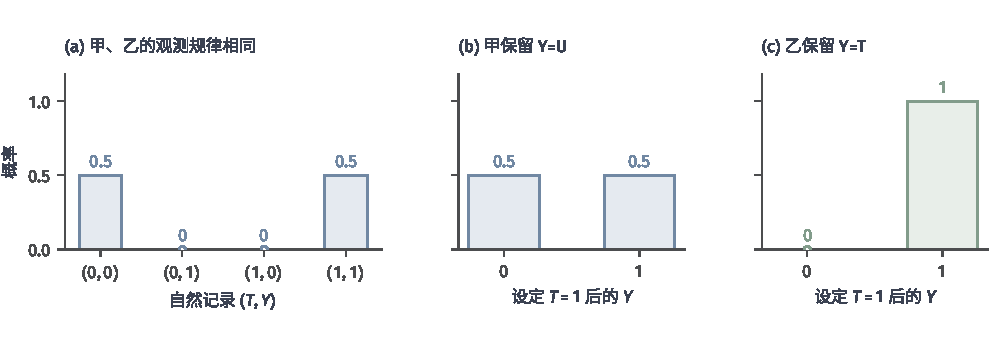
\includegraphics[width=169mm]{figures/00-shared/mathematical-preliminaries-lower/01-random-variables-distributions-and-causality/matplotlib/causal-identical-observation-different-intervention/figure.pdf}
  \caption{相同自然记录与不同的干预响应。背景\(U\sim\operatorname{Bernoulli}(1/2)\)，两模型都有\(T=U\)，但甲的结果规则为\(Y=U\)，乙为\(Y=T\)。左图给出两模型共同的自然联合概率；中、右图均把处理规则替换成\(T=1\)，分别保留各自的结果规则。所有柱高是给定教学机制的精确总体概率，共用概率尺度；中、右两图不是从左图按\(T=1\)筛选得到的条件分布。}
  \label{fig:causal-identical-observation-different-intervention}
\end{figure*}

\subsection{机制干预下的潜在结果}
\label{sec:causal-intervention-potential-outcomes}

在二元例子中，行动直接把\(T=U\)换成\(T=t\)，并沿用原来的结果规则。这项替换就是机制干预：它规定处理如何产生，再让保留的规则使用新的处理值。相同的观测条件概率没有记录这项替换，因此干预需要单独的模型约定。

\begin{definition}[理想干预]
  \label{def:causal-intervention}
  对给定模型的处理变量\(T\)作\term{干预}（intervention）
  \(\operatorname{do}(T=t)\)，表示删除自然生成\(T\)的规则，并以常量规则
  \(T=t\)替换。其余生成规则和指定的背景分布\(P_{\bm U}\)保持不变。
  由行动映射\(F_M^{a(t)}\)推前得到的分布记作
  \(P^{\operatorname{do}(T=t)}\)。
\end{definition}

“其余规则不变”不是说其余变量的取值不变。理解这一点的关键是：干预替换的是“处理怎样产生”这一条规则，而不是把其他变量的当前值冻结；所有以处理为输入的下游变量都要拿着新的处理值按各自原规则重新算一遍。若培训改变技能，技能再影响成绩，
行动后技能和成绩都应重算。只锁住所有非处理字段再评估一个预测器，通常不是这一行动。
多变量行动同样由\(F_M^a\)表达，但模型必须说明哪些规则替换、哪些保留。

干预已经确定怎样替换规则。现在仍从同一个背景总体分布抽取一个单位，并在所抽背景上执行指定处理，所得结果就成为一个随机变量。对同一单位比较两项处理时，两次计算必须复用同一个背景，才能表示这个单位本会得到的两种结果。
\begin{definition}[潜在结果]
  \label{def:causal-potential-outcomes}
  对明确的目标总体、处理版本和结果测量时间，\term{潜在结果}
  （potential outcome）是随机变量
  \begin{equation}
    Y(t)=R_M(t,\bm U).
    \label{eq:causal-response-potential-outcome}
  \end{equation}
  对二元处理，\((Y(0),Y(1))\)定义在同一背景概率空间上；两项分别表示同一单位
  在两种处理下的结果，而不是分别抽取两个人。
\end{definition}

这里的关键是“同一单位、两种安排”的对比：\(Y(1)\)和\(Y(0)\)是同一个人在两种平行情形下本会取得的成绩，二者之差才干净地反映培训对这个人的作用；如果拿参加培训的一群人和另一群没参加的人比，差异里还混着两群人本来的基础差距。
可测性保证可以讨论潜在结果的概率规律。记\(\mathcal L(Z)\)为随机变量\(Z\)的分布，
则
\[
  \mathcal L(Y(t))
  =
  (R_M(t,\cdot))_{\#}P_{\bm U}
  =
  \mathcal L(Y\mid\operatorname{do}(T=t)).
\]
符号\(\#\)表示\BookSectionRef{sec:rv-pushforward}{第~\ref{sec:rv-pushforward}节}的分布推前。这里的
\(\operatorname{do}\)标记修改后的模型，不是对自然事件\(T=t\)作普通条件化。
潜在结果聚焦所选行动下的输出；仅有一张潜在结果表，并不自动给出其他变量的完整
生成机制\scite{math-hernan2020whatif}

观察条件分布\(p(y\mid T=t)\)会筛选自然规则恰好给出处理\(t\)的单位，因而同时
包含处理作用和进入处理组的选择。在上面两套机制中，都有
\[
  \mathbb P(Y=1\mid T=1)=1,\qquad
  \mathbb P(Y=1\mid T=0)=0.
\]
但对甲，设定处理以后结果仍为\(U\)，故
\[
  \mathbb P(Y=1\mid\operatorname{do}(T=t))=\frac12,
  \qquad t\in\{0,1\};
\]
对乙，设定处理以后结果为\(t\)，故
\[
  \mathbb P(Y=1\mid\operatorname{do}(T=t))=t.
\]
相同的观测关联对应不同的行动后果。缺少的是关于响应机制的约束，不是更精确地估计
已经相同的两个条件概率。

固定处理值并非唯一行动。\term{随机干预}（stochastic intervention）用新的随机
规则替换处理规则，例如给定处理前信息\(X=x\)时，按概率核\(q(\cdot\mid x)\)安排培训。
这里\(q\)是从信息空间到处理空间的可测概率核。若这两个空间均为标准Borel空间，
可以加入独立于原背景的\(W\sim\operatorname{Unif}(0,1)\)，选取可测函数\(g_q\)，
使\(T=g_q(X,W)\)在给定\(X\)后的分布为\(q(\cdot\mid X)\)，再运行保留的机制。
有限处理空间中，这个构造就是按\(q\)的累计概率划分\([0,1]\)，读取\(W\)落在哪一段；
一般标准Borel空间则由概率核的随机化表示保证这样的可测实现。
若不满足这些空间条件，应直接以概率核的替换定义干预，不默认已有函数\(g_q\)。
确定性策略是新规则不再需要随机化的特例。随机化是否独立、行动可使用哪些信息，
都是干预定义的一部分；仅把某个概率因子改写为\(q\)不能保证其余现实机制未变。
局部机制成立时相应的分解公式在第~\ref{sec:causal-mechanism-composition}节建立。

\subsection{观测结果与干预响应的连接}
\label{sec:causal-response-observation-link}

一名接受培训的人的实际成绩，能否作为\(Y(1)\)的记录，取决于潜在结果所指的培训方案是否与实际执行一致。不同课程、时长和测量日期会给出不同的结果变量；先把这些条件固定，才能把记录接到相应的潜在结果上。对多名参与者，还要说明一人的处理是否会改变其他人的成绩。

这两项要求各管一件事。第一项要保证“\(Y(1)\)”这一记号指的是这个人实际接受的那种培训，
而不是另一种同名却内容不同的方案；若记录中的\(T=1\)对应的课程与潜在结果定义时的
课程不一致，两者就无法接到一起。第二项要保证一个人的成绩不受其他人处理的影响，
否则\(Y_i\)还要依赖整组人的处理安排，只比较\(t_i\)就不足以概括后果。
下面的定义把这两点分开写出。

\begin{definition}[处理一致性与无干扰]
  \label{def:causal-consistency-no-interference}
  对明确的处理版本，\term{一致性}（consistency）要求实际处理对应的结果满足
  \(Y=Y(T)\)几乎必然成立；特别地，
  \begin{equation}
    \begin{gathered}
      T=t\Longrightarrow Y=Y(t),\\
      \text{二元处理且结果为实数或实向量时，}\quad Y=TY(1)+(1-T)Y(0).
    \end{gathered}
    \label{eq:causal-consistency}
  \end{equation}
  对\(n\)个单位，无干扰要求：每个\(i\)及任意两个处理向量
  \(\bm t,\bm t'\)，只要\(t_i=t_i'\)，就有
  \(Y_i(\bm t)=Y_i(\bm t')\)几乎必然成立。因此单位\(i\)的潜在结果才可简记为
  \(Y_i(t_i)\)。
\end{definition}

一致性连接自然记录与行动响应，没有把未采取行动的结果变成可见记录。若模型给出
自然处理\(T=F_{M,T}(\bm U)\)，这一条件要求自然结果与
\(R_M(F_{M,T}(\bm U),\bm U)\)相合；不能任意拼接不相容的自然函数与响应族。
在依规则替换而构造的无环模型中，这种相合性可以逐方程检查。

无干扰则限制研究单位之间的相互作用。疫苗接种、社交网络和市场竞争中，一人的行动
可能改变他人的暴露或机会；此时\(Y_i(\bm t)\)往往依赖整个处理向量。
例如\(Y_i(\bm t)=t_i+\eta\sum_{j\ne i}t_j/(n-1)\)在
\(n>1,\eta\ne0\)时不满足无干扰。可以另行规定网络暴露、分组方案或总体处理比例，
但不能继续把只比较\(t_i\)的效应解释为所有联动后果。

通常所说的稳定单位处理值假设把处理版本唯一性和无干扰合在一起。它们与分配机制仍
须分开判断：分配机制规定\(T\)怎样依赖\(X,Y(0),Y(1)\)等量，一致性只连接实际
处理与观察结果。即使处理版本清楚且单位互不干扰，主动选择培训的人也可能具有不同
背景。响应的表示到此已建立，能否由这种选择后的观测恢复响应，是后面识别部分的问题。

\section{因果响应的比较与变化}
\label{sec:causal-response-comparison}

培训对不同人的作用可能方向相反，平均成绩也可能掩盖低分概率的变化。比较之前需要确定查询：同一人改变处理会差多少，对目标人群平均会差多少，还是结果分布某个部分会怎样移动。下面固定模型、处理版本与总体，分别给这些比较建立量；连续剂量的导数再说明当前剂量附近的小变化。

\subsection{同一背景下的响应比较}
\label{sec:causal-individual-response}

已经给定\(R_M\)时，计算同一人的两种结果只改变处理值\(t\)，背景\(\bm u\)保持不动。对实值成绩，可以直接相减；所得差值刻画这一背景下的处理作用，而不是两名不同人的成绩差。

\begin{definition}[同一背景下的响应差]
  \label{def:causal-individual-effect}
  对实值结果及允许的处理值\(t,t'\)，固定背景\(\bm u\)的响应差定义为
  \begin{equation}
    \Delta_M(t,t';\bm u)=R_M(t,\bm u)-R_M(t',\bm u).
    \label{eq:causal-individual-response-difference}
  \end{equation}
  二元处理的\term{个体处理效应}（individual treatment effect）是随机变量
  \(Y(1)-Y(0)=\Delta_M(1,0;\bm U)\)。
\end{definition}

这里的减法保持同一背景，而不是用一个处理组成员减去另一个未处理组成员。
例如\(R_M(t,u)=u+(2u-1)t\)，其中\(u\in\{0,1\}\)。对背景\(u=1\)，处理使
结果增加\(1\)；对\(u=0\)，处理使结果减少\(1\)。比较两名不同背景个体的实际
结果，还混入了基础值\(u\)的差异。

给定模型和背景时，两个响应都可以计算。但现实中一个人在同一时刻只能真实处在一种处理下，因此每个单位的实际记录只能包含
\(Y(T)\)，不会同时包含同一时刻的\(Y(1)\)与\(Y(0)\)：参加了培训就看不到他“假如没参加”的成绩，反之亦然。这就是因果推断里常说的“因果推断的根本难题”。因此“个体效应有明确定义”
与“它能由该人的一次观察确定”是两件事。即使已知某人当前结果为零，仍需要机制或
关于背景的信息才能计算另一行动下的结果。

对向量结果，可以先报告各坐标差，也可以指定具有实质含义的效用函数
\(h:\mathcal Y\to\mathbb R\)，比较
\(h(R_M(t,\bm u))-h(R_M(t',\bm u))\)。对类别结果，直接相减通常没有意义，
可以比较某事件的指示量。选择\(h\)是在规定目标，不是纯粹的记号替换：
提高收入、降低风险和同时满足两项要求，可能给出不同的行动排序。

\subsection{背景总体下的响应比较}
\label{sec:causal-population-response}

如果目标是决定一项培训是否适用于指定人群，两项行动都应按目标人群的同一个背景分布平均。这样得到的是总体作用，允许不同背景的个体效应互相抵消。保留完整结果分布还能看到均值没有显示的变化，例如成绩的尾部或分位数；两种报告服务于不同决策问题。

\subsubsection{总体与条件总体的平均响应比较}
\label{sec:causal-average-response}

个体效应\(Y(1)-Y(0)\)因人而异，决策者通常看不到也不需要每个人的确切效应，而是关心“对目标人群平均而言，培训值不值得推广”。把所有人在两种安排下的平均成绩相减，就得到这个总体尺度；计算时仍须让两种平均使用同一批人的背景分布，而不是比较两群不同的人。
\begin{definition}[平均处理效应]
  \label{def:causal-average-treatment-effect}
  对二元处理，假设\(Y(0),Y(1)\)都可积，\term{平均处理效应}
  （average treatment effect, ATE）定义为
  \begin{equation}
    \tau
    =
    \mathbb E[Y\mid\operatorname{do}(T=1)]
    -
    \mathbb E[Y\mid\operatorname{do}(T=0)].
    \label{eq:causal-ate-interventional}
  \end{equation}
\end{definition}

两个干预总体使用同一个\(P_{\bm U}\)。由潜在结果与干预分布的对应关系及期望线性性，
\begin{equation}
  \tau
  =\mathbb E[Y(1)-Y(0)]
  =\mathbb E[Y(1)]-\mathbb E[Y(0)].
  \label{eq:causal-ate-potential-outcomes}
\end{equation}
可积性排除了\(\infty-\infty\)这样的未定义运算。线性期望说明计算平均差只需要两个
边缘均值，并没有使同一单位的两个结果同时可见。上例若
\(\mathbb P(U=1)=\mathbb P(U=0)=1/2\)，ATE为零，但没有人的个体效应为零。

总体平均把受益和受损的人抵消成一个数，可能掩盖“培训对某类人特别有效、对另一类人无效甚至有害”。若要辨认哪些人可能受益、从而因人而异地安排处理，可以在处理前协变量\(X\)下分层，只对具有相同可观测特征的人平均效应。
\begin{definition}[条件平均处理效应]
  \label{def:causal-conditional-average-effect}
  设\(X\)在所比较干预下保持同一取值与含义，且两种潜在结果可积。
  \term{条件平均处理效应}（conditional average treatment effect, CATE）是
  \begin{equation}
    \tau(x)=\mathbb E[Y(1)-Y(0)\mid X=x],
    \qquad P_X\text{几乎处处}.
    \label{eq:causal-cate}
  \end{equation}
\end{definition}
它对具有相同已知特征的人平均，不等于这些人逐个具有相同效应。取
\(X=U\)时，上例的\(\tau(1)=1,\tau(0)=-1\)；若\(X\)未包含\(U\)，
条件平均仍可能掩盖层内差异。不能把处理后的技能水平直接当作这里不随行动变化的
\(X\)：按两种行动各自产生的技能筛人，通常不是比较同一条件总体。

全期望给出\(\tau=\mathbb E_X[\tau(X)]\)。若响应机制不变而目标总体从\(P_X\)
换为\(Q_X\)，且对应的条件背景规律与条件效应保持不变，新ATE为
\(\int\tau(x)Q_X(\mathrm dx)\)。这是人群权重的变化，不是机制突然发生改变；
条件效应能否跨总体保留本身仍需假设。目标总体、处理版本或测量时间改变，都应重新
标明效应的含义。

对有限处理集合\(\mathcal T\)，同样定义
\[
  \tau(t,t')=\mathbb E[Y(t)-Y(t')].
\]
若行动由处理前信息决定，则要比较整个策略。本段把同一处理\(T\)的允许取值组成
有限动作集合\(\mathcal A\subseteq\mathcal T\)，用处理值\(a\)标记“设定\(T=a\)”
这项行动。因此这里的\(Y(a)=R_M(a,\bm U)\)沿用潜在结果的定义；本段尚未把
\(a\)扩展为同时替换多项机制的一般行动。仍假定\(X\)不随这些处理行动改变。
策略\(\pi(a\mid x)\)用独立于原背景的新增随机化，在给定\(X=x\)时选择处理值\(a\)。
将\(\pi\)在\(\mathcal T\setminus\mathcal A\)上延拓为零，表示策略不会选择这些
处理值；这样以后即使对自然记录中的处理值求\(\pi(T\mid X)\)，记号也有定义。
在所有潜在结果可积时，它的单步价值为
\begin{equation}
  V(\pi)=\mathbb E_X\left[
    \sum_{a\in\mathcal A}\pi(a\mid X)\mathbb E[Y(a)\mid X]
  \right].
  \label{eq:causal-policy-value}
\end{equation}
式中独立随机化保证选择动作不会额外按未观测背景筛人。确定性策略是
\(\pi\)集中于一个动作的特例。这里定义的是给定模型内的目标；多值处理需要哪些
观测覆盖、策略可使用哪些已有记录，在第~\ref{sec:causal-effect-identification}节
再检查。连续剂量也不能被当作每个精确值都具有正概率的离散组。

\subsubsection{干预结果的分布响应比较}
\label{sec:causal-distribution-response}

平均值只记录分布的一个特征。设\(U\)等概率取\(-1,1\)，
\(Y(0)=0,Y(1)=U\)，则ATE为零，但处理后从人人得到零变成两种相反结果。
若低于零代表失败，未处理时的失败概率为\(0\)，处理后却为\(1/2\)。
均值虽相同，失败概率的变化仍会影响按风险选择行动的决策。

对实值结果，定义干预分布函数与其广义分位数
\[
  F_t(y)=\mathbb P(Y(t)\leq y),\qquad
  Q_t(p)=\inf\{y:F_t(y)\geq p\},\quad 0<p<1.
\]
\(F_t(y)-F_{t'}(y)\)比较不高于阈值的概率，\(Q_t(p)-Q_{t'}(p)\)比较两个总体
处于同一分位位置的结果。后者并不是个体效应
\(Y(t)-Y(t')\)的第\(p\)分位数，因为处于两个分布相同排名的未必是同一个人。
只有额外规定跨行动的排序对应关系，才能把这种配对解释成个体变化。

也可以使用第~\ref{chap:information-theory-and-statistical-geometry}章的分布比较
尺度。总变差比较事件概率而不要求矩；采用\(p\)阶Wasserstein距离时应满足所用
空间和有限\(p\)阶矩条件；使用KL散度则须检查绝对连续性及其值是否有限。
尺度的选择服务于所关心的风险或损失，不能用一个小均值差代替所有分布都接近。

两个干预边缘即使完全已知，仍没有说明它们如何在同一背景上配对。
第~\ref{sec:causal-factual-counterfactual}节将用两张联合表说明：分布比较足以回答
部分总体问题，却不足以回答已知某人事实结果后的替代结果。

\subsection{连续处理下的局部响应变化}
\label{sec:causal-local-response}

二元处理只能比较“做”与“不做”；当处理是药物剂量、培训时长、利率这类连续量时，还可以提出更细的问题：“在当前剂量上再增加一点点，结果大约改变多少？”这正是微积分里导数在因果响应上的对应物——它描述当前剂量附近的局部响应，而不是任意两个相差很大的剂量之差。
二元处理适合比较有无行动；连续剂量还可以询问“在当前剂量附近再增加一点会怎样”。
局部线性近似把小输入增量的响应写成线性主部与高阶余项；这里用它描述固定模型、
固定背景下的响应变化，而不是观测人群随剂量改变产生的回归变化。相关的可微性与
线性近似工具可参考
\BookChapterRef{chap:univariate-differentiation}{卷1《数学准备：计算、分析与几何》的“一元函数的微分”章}。

\begin{definition}[局部响应导数]
  \label{def:causal-local-response}
  设处理取值位于开集\(\mathcal T\subseteq\mathbb R^k\)，结果位于
  \(\mathbb R^m\)。用粗体标明向量剂量；若
  \(\bm t\mapsto R_M(\bm t,\bm u)\)在\(\bm t_0\)可微，其局部响应
  Jacobian为\(D_{\bm t}R_M(\bm t_0,\bm u)\)，满足
  \[
    R_M(\bm t_0+\bm h,\bm u)-R_M(\bm t_0,\bm u)
    =D_{\bm t}R_M(\bm t_0,\bm u)\bm h+o(\|\bm h\|).
  \]
  标量处理、标量结果时记为\(\partial_tR_M(t_0,\bm u)\)。
\end{definition}

该导数是每单位剂量的局部变化，不是任意有限剂量差。比如
\(R_M(t,u)=u+t^2\)，从\(t=1\)增加到\(1+h\)的响应差是\(2h+h^2\)，
局部导数为\(2\)。\(h\)很小时一阶项有用，但从\(1\)变到\(2\)的差为\(3\)，
不能直接用导数值\(2\)代替。离散行动没有这样的邻域，仍应使用有限差。

图~\ref{fig:causal-local-response-tangent}把这两个比较放在同一背景\(u=0\)下。切线只在\(t=1\)附近提供一阶近似；连接\(t=1\)与\(t=2\)的割线则累计了整个剂量区间内的响应变化。响应曲线弯曲时，割线斜率一般不等于起点处的导数。

\begin{figure}[htbp]
  \centering
  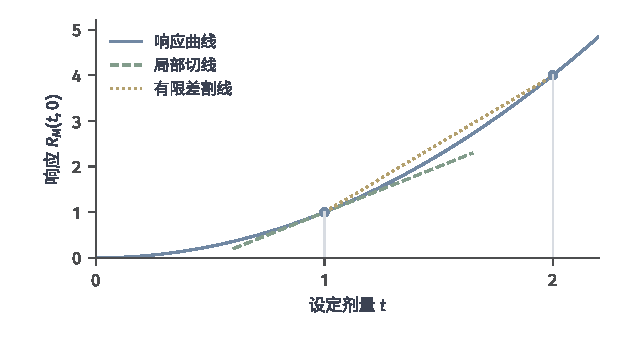
\includegraphics[width=105mm]{figures/00-shared/mathematical-preliminaries-lower/01-random-variables-distributions-and-causality/matplotlib/causal-local-response-tangent/figure.pdf}
  \caption{固定背景下的局部导数与有限剂量差。蓝实线为\(R_M(t,0)=t^2\)，绿虚线为\(t=1\)处斜率为\(2\)的切线；黄点线连接\((1,1)\)和\((2,4)\)，割线斜率为\(3\)。本例剂量差恰为\(1\)，所以有限响应差也为\(3\)；一般剂量差下还须除以剂量增量才得到割线斜率。}
  \label{fig:causal-local-response-tangent}
\end{figure}

总体平均响应\(m(t)=\mathbb E[R_M(t,\bm U)]\)还包含积分，不能仅凭每个人的
响应可微就交换求导与期望。下面给出一个可以直接检查的充分条件。
\begin{theorem}[平均响应的求导]
  \label{thm:causal-response-differentiation}
  设\(I\)是包含\(t_0\)的开区间，\(R_M(t_0,\bm U)\)可积。若对几乎每个
  \(\bm u\)，\(R_M(\cdot,\bm u)\)在\(I\)可微，且存在非负可积函数
  \(g(\bm U)\)，使
  \[
    |\partial_tR_M(t,\bm u)|\leq g(\bm u),
    \qquad t\in I,
  \]
  则\(m\)在\(t_0\)可微，且
  \begin{equation}
    m'(t_0)=\mathbb E[\partial_tR_M(t_0,\bm U)].
    \label{eq:causal-average-response-derivative}
  \end{equation}
\end{theorem}
\begin{proof}
  对足够小的非零\(h\)，中值定理给出
  \[
    \left|
      \frac{R_M(t_0+h,\bm u)-R_M(t_0,\bm u)}{h}
    \right|\leq g(\bm u).
  \]
  因而\(R_M(t_0+h,\bm U)\)可积，且差商几乎处处收敛到
  \(\partial_tR_M(t_0,\bm U)\)。可积的\(g\)统一控制这些差商，支配收敛定理
  允许将极限移入期望，得到
  \[
    \lim_{h\to0}\frac{m(t_0+h)-m(t_0)}{h}
    =
    \mathbb E\!\left[
      \lim_{h\to0}
      \frac{R_M(t_0+h,\bm U)-R_M(t_0,\bm U)}{h}
    \right],
  \]
  即所述结论。
\end{proof}

向量处理可以在相应可积控制下逐坐标求导；若要得到完整可微性，则需足以控制
Jacobian及余项的邻域条件。上述定理把“个体可微”与“可交换积分”分开，
后者限制少量背景下异常陡峭的响应，避免其破坏总体极限。

局部响应导数也不等于观测回归斜率
\(\partial_t\mathbb E[Y\mid T=t,X=x]\)。后者随\(t\)改变的还可能是自然进入
该剂量的人群。第~\ref{sec:causal-sensitivity-ranges}节以总体线性投影系数为例计算混杂偏差；这一系数一般也不等于上述逐点导数。
它同样不同于随机轨道的It\^o微分：这里对可设定输入作普通局部变化，背景固定；
随机轨道微分描述随时间累积的随机变化，一般不存在普通逐轨道时间导数。
因此模型的光滑性支持局部计算，却不同时保证这个导数能由观测识别或能外推到大幅行动。

\section{给定事实后的因果响应}
\label{sec:causal-counterfactual-recourse}

假设某人的处理、成绩和其他记录已经可见，我们希望判断另一行动会给他带来什么结果。此时不能重新从人群中抽取背景，因为事实已经排除了一些可能的背景。固定模型后，先由事实获得背景条件分布，再用替代行动映射同一组可能背景；反事实和行动补救都从这项条件化计算出发。

\subsection{事实条件下的反事实计算}
\label{sec:causal-factual-counterfactual}

给定事实\(\bm E=\bm e\)，所求对象是这个单位在替代行动下的条件结果。模型将自然记录与替代结果放在同一背景\(\bm U\)上，事实用于限定\(\bm U\)，行动用于改变生成规则；这两个操作需要分别保留。

\begin{definition}[给定响应模型的反事实变量]
  \label{def:causal-counterfactual}
  设模型\(M\)具有定义~\ref{def:causal-response-interface}的自然映射\(F_M\)及
  行动映射\(F_M^a\)。在同一外生背景\(\bm U\)上，\term{反事实}
  （counterfactual）变量定义为\(\bm V_a=F_M^a(\bm U)\)。
  给定实际证据\(\bm E\)后的反事实分布是\(\bm V_a\)关于该证据的条件分布，
  而不是重新按背景总体抽取一个人。
\end{definition}

事实证据可来自自然变量的一部分，也可包括带噪测量；后一情形把测量随机性一并纳入
背景，使证据的生成规则明确。反事实计算通常概括为三步——“溯因、干预、预测”，可以用一个例子体会：看到一名学生实际没参加培训却考了 70 分，先根据这个成绩反推他可能属于哪种能力水平（溯因，得到能力的条件分布）；再在脑海中把“是否参加培训”改成“参加”（干预，切换行动规则）；最后用更新后的能力和新规则重新推算他的成绩（预测）。
溯因由事实得到背景条件分布，干预切换到允许的行动映射，预测将同一个背景条件分布
推到结果空间。这里的溯因是给定模型内的条件化，并不是由一条记录证明模型正确。

设空间允许选取正则条件分布
\(P_{\bm U\mid\bm E=\bm e}\)，例如本章常用的标准Borel空间。按联合分布等于边缘分布与条件分布相乘的分解（离散与密度情形可参考\BookSectionRef{sec:rv-conditional-distribution}{第
~\ref{sec:rv-conditional-distribution}节}），对任意可测集合\(B\)，三步合成为
\begin{equation}
  \begin{aligned}
    \mathbb P(\bm V_a\in B\mid\bm E=\bm e)
    &=
    \bigl((F_M^a)_{\#}
      P_{\bm U\mid\bm E=\bm e}\bigr)(B)\\
    &=
    \int\mathbb I\{F_M^a(\bm u)\in B\}
      P_{\bm U\mid\bm E=\bm e}(\mathrm d\bm u).
  \end{aligned}
  \label{eq:causal-counterfactual-pushforward}
\end{equation}
式中事实只进入背景条件分布，行动只进入映射。连续证据点通常概率为零，等式按所选
正则条件分布版本理解，只保证对证据分布几乎处处的\(\bm e\)成立。在一个指定的
零概率证据点上报告数值，还需要选定版本或连续性等额外结构；积分恒等式本身不能
唯一规定每个点的条件值。

考虑已经明确给定的教学模型
\begin{equation}
  X=U_X,\qquad
  T=f_T(X,U_T),\qquad
  Y=2X+3T+U_Y.
  \label{eq:causal-counterfactual-linear-example}
\end{equation}
它直接提供自然映射及替换处理规则后的映射。某人的事实为
\(X=2,T=0,Y=5\)，于是
\[
  U_Y=5-2\times2-3\times0=1.
\]
保持该人的\(X,U_Y\)不变，把处理设为\(1\)，得到
\[
  Y_{T\leftarrow1}=2\times2+3\times1+1=8.
\]
差值\(3\)来自给定结果规则中的处理作用。事实不必确定全部背景，例如可能仍不知道
\(U_T\)；只要未确定部分不影响本次行动后的结果，仍能得到这个点值。
若结果规则不确定，或未确定的背景继续进入结果，则应给出条件分布或范围。

\begin{example}[两点背景后验的反事实推前]
  \label{ex:causal-two-point-background-posterior}
  令背景类型\(U\in\{u_{\mathrm L},u_{\mathrm H}\}\)先验概率各为\(1/2\)。
  事实中观察到二元信号\(S=1\)，且模型规定
  \[
    \mathbb P(S=1\mid U=u_{\mathrm H})=\frac34,\qquad
    \mathbb P(S=1\mid U=u_{\mathrm L})=\frac14.
  \]
  因而\(\mathbb P(S=1)=\frac12(\frac34+\frac14)=\frac12\)，Bayes公式给出
  \[
    \mathbb P(U=u_{\mathrm H}\mid S=1)=\frac34,\qquad
    \mathbb P(U=u_{\mathrm L}\mid S=1)=\frac14.
  \]
  若行动\(a\)下的结果在两类背景中分别为
  \(F_{M,Y}^a(u_{\mathrm L})=2,F_{M,Y}^a(u_{\mathrm H})=6\)，则
  \[
    \mathcal L(Y_a\mid S=1)=\frac14\delta_2+\frac34\delta_6,\qquad
    \mathbb E[Y_a\mid S=1]=\frac14\,2+\frac34\,6=5.
  \]
  忽略事实而按先验重新抽取背景，得到总体干预分布
  \(\frac12\delta_2+\frac12\delta_6\)，均值为\(4\)。
  两个答案使用同一行动映射，只是反事实计算保留了事实提供的背景信息。
\end{example}

这个例子也可放回完整背景接口：另加独立测量随机量生成信号\(S\)，行动结果只依赖
类型\(U\)，于是积分掉测量背景就得到上面的两点后验。未知背景不必被硬选成某一类。

图~\ref{fig:causal-abduction-intervention-prediction}并列展示这两条推前路径：条件反事实保留事实形成的后验，总体干预沿用背景先验。

\begin{figure*}[htbp]
  \centering
  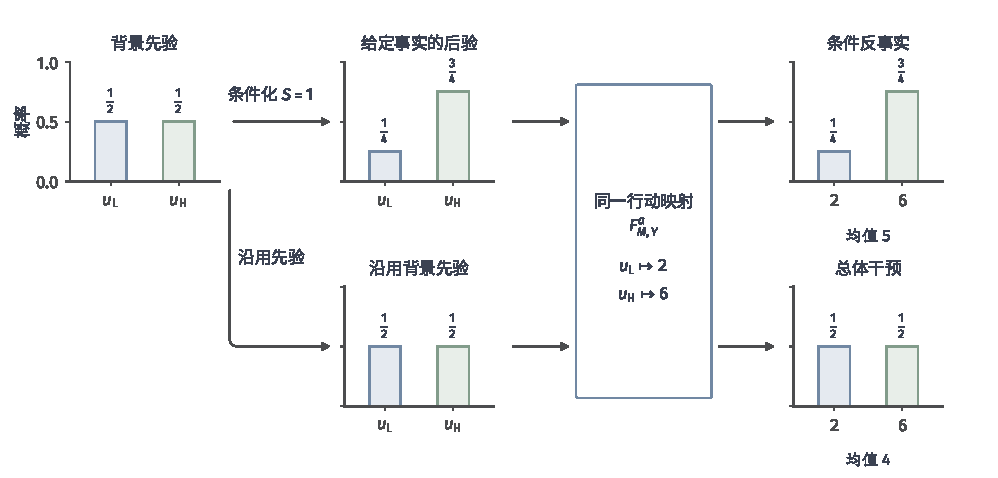
\includegraphics[width=169mm]{figures/00-shared/mathematical-preliminaries-lower/01-random-variables-distributions-and-causality/matplotlib/causal-two-point-pushforwards/figure.pdf}
  \caption{同一行动映射下的条件反事实与总体干预。背景$u_{\mathrm L},u_{\mathrm H}$的先验概率各为$1/2$，
  事实$S=1$将两者的后验概率更新为$1/4,3/4$；行动映射分别给出结果$2,6$。
  保留后验得到条件均值$5$，沿用先验得到总体干预均值$4$。
  概率柱使用共同的零基线与比例尺；溯因是给定模型内的条件化，不证明结构假设本身有效。}
  \label{fig:causal-abduction-intervention-prediction}
\end{figure*}


还有一种更深的歧义：即使知道两种行动各自的总体分布，也未必知道同一个人的两个
结果怎样配对。设两种干预结果均为\(\operatorname{Bernoulli}(1/2)\)。
模型甲令一半单位满足\((Y(0),Y(1))=(0,0)\)，另一半满足\((1,1)\)；
模型乙令两类单位分别满足\((0,1)\)和\((1,0)\)。甲的个体效应恒为零，
乙的个体效应等概率取\(1,-1\)，而两模型的ATE都为零。

图~\ref{fig:causal-cross-world-couplings}给出了对应的联合概率表。用定义
~\ref{def:information-coupling}的语言，两者是相同边缘的不同耦合。
已知\(Y(0)=0\)时，甲给\(Y(1)=0\)，乙给\(Y(1)=1\)。在独立随机分配处理
的事实世界里，把同一事实\(T=0,Y=0\)分别输入两套模型，会得到不同的条件反事实。
这项计算比较的是模型给出的答案，并没有用该事实区分两套模型。

\begin{figure}[htbp]
  \centering
  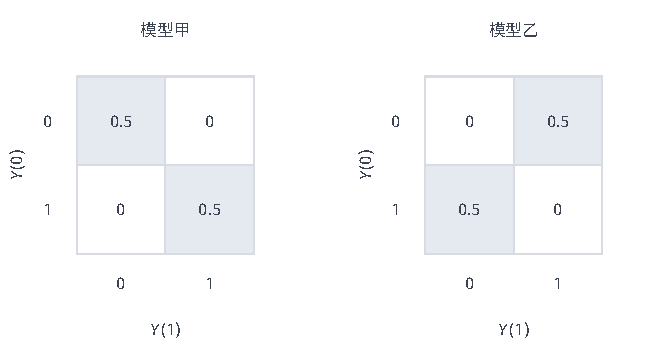
\includegraphics[width=\linewidth]{figures/00-shared/mathematical-preliminaries-lower/01-random-variables-distributions-and-causality/tikz/causal-cross-world-couplings/figure.pdf}
  \caption{相同干预边缘的两种跨世界配对。行对应\(Y(0)\)，列对应\(Y(1)\)，格内
  数字为联合概率；每张表的行和、列和均为\(1/2\)。甲的个体效应恒为零，乙的个体
  效应等概率取\(1,-1\)，两者ATE均为零。这是相容机制的教学构造，不是随机试验
  直接观察到的潜在结果联合表。}
  \label{fig:causal-cross-world-couplings}
\end{figure}

两套配对连完整随机试验的两组边缘也无法区分。要回答条件个体反事实，还需要关于
跨世界联合结构的机制限制，或具有适当稳定性、时间和携带效应假设的重复干预资料；
否则应保留相容范围。模型明确给定时可以用式
~\eqref{eq:causal-counterfactual-pushforward}计算，可观测分布与机制假设是否足以确定这套模型则是
第~\ref{sec:causal-effect-identification}节的另一个问题。

\subsection{目标约束下的行动补救}
\label{sec:causal-action-recourse}

反事实计算还可以反过来服务于行动选择：当模型预测某人会被拒绝（比如贷款申请未通过），他自然想问“我该做些什么才能通过审核”，而这些改变应当是现实中真正能做到的。这就是行动补救要解决的问题——怎样以尽量低的代价，让同一个人的决策
达到目标？先要区分两种看似相近、实则不同的操作。对预测器\(\widehat y=f(x,t)\)，输入替换给出
\[
  f(x,1)-f(x,0).
\]
这只是已训练函数对字段变化的响应，相当于在计算器里把一个输入数字改掉再看输出，并不考虑现实中改变这个字段会牵动什么。若现实培训提高技能、同时占用工作时间，那么
只改“是否培训”一列而锁住技能和时间，通常不是任何可实施的行动结果。

\begin{definition}[因果行动补救]
  \label{def:causal-recourse}
  给定事实证据\(\bm E=\bm e\)，以\(x=\xi(\bm e)\)表示由事实确定的行动信息摘要，
  其中\(\xi\)为预先指定的可测映射。给定可实施行动集合\(\mathcal A(x)\)、响应模型、行动成本\(c(a;x)\)
  与目标决策集合\(G\)，\term{行动补救}（algorithmic recourse）寻找能够使行动后
  的决策落入\(G\)的可行行动。因果行动补救用同一背景下的干预状态
  \(\bm V_a=F_M^a(\bm U)\)评价成功条件，并按机制重算所有受行动影响的状态。
\end{definition}

令\(d\)为最终决策规则。若事实唯一确定背景\(\bm u\)，优化形式为
\begin{equation}
  \min_{a\in\mathcal A(x)}c(a;x)
  \quad\text{使得}\quad d(F_M^a(\bm u))\in G.
  \label{eq:causal-recourse-objective}
\end{equation}
可行集合规定实际允许做什么，成本规定如何比较行动，成功约束规定要得到何种决策。
这三项共同规定一个约束优化问题，不能只用一个距离函数代替。低输入距离不等于低行动成本；不可改变属性也不应成为行动建议。
若可行集合为空，应报告无法在当前约束下补救，而不是输出一个不可执行的最近点。
相关工具可参考\BookChapterRef{chap:optimization}{卷1《数学准备：计算、分析与几何》的“最优化”章}。

多数事实只能给出背景条件分布。给定可容许失败概率\(\alpha\in[0,1]\)，可以采用
概率型约束
\begin{equation}
  \mathbb P\bigl(d(F_M^a(\bm U))\in G\mid\bm E=\bm e\bigr)
  \geq1-\alpha.
  \label{eq:causal-recourse-probability}
\end{equation}
这个条件要求失败背景集合的后验概率至多为\(\alpha\)。回到例
~\ref{ex:causal-two-point-background-posterior}，若目标是\(Y_a\geq5\)，行动\(a\)
的后验成功概率为\(3/4\)，因此在\(\alpha=1/4\)时满足概率约束；但低类型背景的
结果为\(2\)，这一类仍与事实相容的背景全部失败。只挑高类型作为“代表背景”会
漏掉这项风险。

若要求每个保留下来的背景都成功，就需要比允许少量失败更强的逐点约束。为此先要
说明保留哪些背景。离散情形可保留每个具有正后验概率的背景；连续情形的单点可能
都是零概率，不能用单点概率判断是否应被保留。给背景空间配上拓扑后，可以保留
那些无论取多小邻域、邻域仍有正条件概率的点，这些点组成条件分布的支持。
若背景空间为Polish空间，且所用条件分布版本是其Borel概率测度，则可说明这个
支持为何覆盖条件概率一。Polish空间有可数拓扑基，
支持以外的点可被可数个零概率开集覆盖；因此支持是闭集且具有条件概率一。
记这个支持为
\[
  \mathcal S_{\bm e}
  =\operatorname{supp}P_{\bm U\mid\bm E=\bm e}.
\]
在这个候选背景集合上要求
\begin{equation}
  d(F_M^a(\bm u))\in G,\qquad \bm u\in\mathcal S_{\bm e},
  \label{eq:causal-recourse-robust}
\end{equation}
这给出支持上的最坏情形保证。该支持具有条件概率一，因此支持上的逐点成功蕴含概率一成功；它还约束支持中
零概率点上的模型取值，因而可能严格更强。一般可测空间没有默认的拓扑支持，
此时应明确给出候选背景集合。若要由该集合上的逐点保证推出概率一成功，
还须要求该集合具有条件概率一。

上面的两点后验支持同时包含高、低两类背景，所以同一行动虽然满足成功概率
\(3/4\)的要求，却不满足支持上的逐点保证。两种约束分别回答“允许多大失败概率”
和“是否覆盖每个保留背景”，应按所需保证选择，不能把前一种达标解释成后一种也达标。

补救也有时间和多人联动的边界。许多人同时接受建议可能改变价格、名额或审核规则；
决策系统更新后，原建议未必仍有效；资源竞争也可能使原先逐人可行的行动无法共同
执行。因此当前模型中存在一个成功行动，不等于建议已经通过现实可行性、持久性
或公平性验证。

\subsection{目标属性干预下的公平补救}
\label{sec:causal-fair-recourse}

设行动已经能改变当前决策，我们还可能要求这种成功不依赖某项受保护属性，例如性别或种族。属性可能经其他变量影响决策，所以只从预测字段中删除属性，并不能保证消除这些影响。给定同一份事实证据后，我们先得到对个体背景的条件分布，再分别改变属性并重新计算它所影响的变量，比较两个属性世界中的预测条件分布。背景全部固定时，两个预测值相同是更强的逐背景要求；下面的定义只要求在同一个事实背景条件分布下，两个预测分布相同，不要求每个未观测背景上的值都相同。哪些属性作用应被排除仍是一项规范选择；给定选择后，模型才规定具体的反事实比较。

令受保护属性为\(A\)，事实证据为\((X=x,A=a)\)。本小节的\(X\)泛指用于推断
背景的其他事实，可能包含属性的后继变量；它不再具有CATE中“处理前且保持不变”
的自动含义。事实中给定\(X=x\)，并不要求替代属性世界的\(X\)仍等于\(x\)。
\begin{definition}[反事实公平]
  \label{def:causal-counterfactual-fairness}
  在给定响应模型与预测规则下，\term{反事实公平}（counterfactual fairness）
  要求：对每个允许的替代属性\(a'\)和每个可测预测值集合\(B\)，以下等式对事实
  证据分布几乎处处的\((x,a)\)成立：
  \begin{equation}
    \begin{aligned}
      &\mathbb P(\widehat Y_{A\leftarrow a}\in B\mid X=x,A=a)\\
      &\qquad=
      \mathbb P(\widehat Y_{A\leftarrow a'}\in B\mid X=x,A=a).
    \end{aligned}
    \label{eq:causal-counterfactual-fairness}
  \end{equation}
  两个属性世界均使用同一个事实背景条件分布，并重新计算由属性影响的状态及预测。
\end{definition}

等式右侧仍以事实\(A=a\)为条件，而不是改用另一群人的证据\(A=a'\)。
只在输入表中替换\(A\)并固定其全部后继变量，检验的是另一个对象。属性干预在这里
是明确模型下的比较操作，也不表示应建议个人改变该属性。

把公平条件加入补救时，为避免与属性值混淆，记补救行动为\(b\)。
要求模型已经规定联合行动映射\(F_M^{b,A\leftarrow a'}\)：对每个属性世界，
保留同一个可比较的行动\(b\)，不对该世界偷偷重新选择更有利的行动。行动与属性
替换须互相兼容，且所比较世界中行动的可实施含义应明确。定义
\[
  \Pi_b^{a'}(B;x,a)
  =
  \mathbb P\bigl(
    d(F_M^{b,A\leftarrow a'}(\bm U))\in B
    \mid X=x,A=a
  \bigr).
\]
一种公平约束补救问题是
\begin{equation}
  \begin{aligned}
    \min_{b\in\mathcal A(x,a)}\quad &c(b;x,a)\\
    \text{使得}\quad
    &\Pi_b^a(G;x,a)\geq1-\alpha,\\
    &\Pi_b^{a'}(\cdot;x,a)=\Pi_b^a(\cdot;x,a)
      \quad\text{对每个允许的 }a'.
  \end{aligned}
  \label{eq:causal-fair-recourse-objective}
\end{equation}
第一项约束要求成功，第二项约束要求同背景的决策分布不随属性改变。也可以另选近似
公平或成本公平目标，但那会改变问题，不能把它们当作上述等式的自动结果。

\begin{example}[成功行动未必满足公平约束]
  \label{ex:causal-fair-recourse}
  设\(A\in\{0,1\}\)，自然培训量为\(B=0\)，资格分数与二元决策规则为
  \[
    K=U+A+B,\qquad d=\mathbb I\{K-2A\geq2\}.
  \]
  可行行动是把培训量设为\(b\in[0,3]\)，成本为\(c(b)=b\)，目标为\(d=1\)。
  已知事实\(A=0,B=0,K=1\)，于是\(U=1\)。在两个属性世界中施加同一行动，
  必须重算\(K\)，得到
  \[
    K_{b,A\leftarrow a'}=1+a'+b,\qquad
    d_{b,A\leftarrow a'}=\mathbb I\{1+b-a'\geq2\}.
  \]
  只要求事实属性下成功时，最小行动为\(b=1\)。但此时\(a'=0\)给决策\(1\)，
  \(a'=1\)给决策\(0\)，并不公平。若同时要求两个属性世界的二元决策相同且
  成功，则必须\(b\geq2\)，故最优行动为\(b=2\)。不行动时两个世界都失败，
  虽然决策相同，却不满足补救目标。
\end{example}

此例检验的是二元决策，不是内部实值分数\(K-2A\)；后者在两个属性世界中始终
相差\(1\)，任何培训量都不能让分数分布相同。公平对象、允许行动及预算都会影响
可行性。对一个已知个体成立的约束，也不自动保证面向所有人的推荐规则公平；
后者还需规定推荐怎样依赖事实，并对其目标人群几乎处处检验。

这些等式均以给定模型为条件。第~\ref{sec:causal-factual-counterfactual}节的
跨世界配对已经说明，相同干预边缘也可能给出不同条件反事实；由观测拟合出一套
生成规则，不等于公平或补救结论已被唯一识别。若多个模型与证据相容，应在该模型类
上报告结论范围。哪些属性或路径属于不应进入决策的因素，则是另需论证的规范选择。
公平要求、解释和行动补救还涉及应用中的现实验证边界，后续章节将继续讨论。
相关工具可参考\BookChapterRef{chap:trust-fairness}{卷3《基础、理论与可信性》第13章“公平性”}、\BookChapterRef{chap:trust-interpretability}{卷3《基础、理论与可信性》第15章“可解释性”}。

\section{因果响应的推断}
\label{sec:causal-effect-identification}

响应计算给出指定模型中的答案，实际研究却可能不知道哪套机制产生了观测。识别先固定可观测分布和机制假设，保留与两者相容的全部模型，再检查这些模型是否给出同一个响应目标。若相同可观测分布对应不同的培训效应，增加按同一制度采集的样本也不能消除该目标的歧义；若所有相容模型给出相同效应，目标才被识别。这里的“相同”指总体观测规律相同，不是两套模型都能产生某一批有限记录。后者仍可能具有不同观测分布，并随重复采样而被区分。把完整生成机制当作候选模型，就回到定义~\ref{def:statistics-identifiability}中的目标可识别性；目标已唯一确定后，再讨论有限样本的估计误差。

这里比较的是“完整生成机制”，不是拟合参数。两套机制可以有完全不同的结构方程和背景分布，
只要它们在已声明的观测制度下给出同一个可观测分布，观测资料就无法分辨它们。
可识别性问的正是：在这些无法分辨的模型之间，目标值是否已经一致。
若一致，说明资料足以确定目标；若不一致，增加同类样本只能把共同的可观测分布估得更准，
并不能消除这层歧义。

记\(P_{\mathrm{obs}}^M\)为模型\(M\)在已声明观测制度下给出的可观测分布，
\(\tau(M)\)为目标。在允许模型类中，若对任意两套模型\(M_1,M_2\)都有
\[
  P_{\mathrm{obs}}^{M_1}=P_{\mathrm{obs}}^{M_2}
  \quad\Longrightarrow\quad \tau(M_1)=\tau(M_2),
\]
就称该目标\term{可识别}（identifiable）。可观测分布可以包括已完成的试验资料，
不必只包括自然观察。目标可识别也不要求模型每个组成部分都唯一确定。

这是总体层面的唯一性，须与有限样本估计、数值计算区分。估计用样本逼近总体量，
计算求出给定表达式或优化问题的答案。一个算法可以精确拟合全部观测条件分布，
却仍无法区分本章开头的两套机制；反过来，目标已有识别式，也不表示样本够多或
数值算法已经稳定。

开篇式~\eqref{eq:causal-observational-equivalence-confounding}与式
~\eqref{eq:causal-observational-equivalence-effect}已经给出可核对的反例：两套模型
都有\(U\sim\operatorname{Bernoulli}(1/2)\)和\(T=U\)，但甲的结果规则为\(Y=U\)，
乙为\(Y=T\)。两者的自然记录都只有\((T,Y)=(0,0),(1,1)\)，概率各为\(1/2\)。
把同一个处理规则替换为\(T=t\)以后，甲仍有\(Y(t)=U\)，乙则有\(Y(t)=t\)，因此
\[
  \begin{aligned}
    \tau(M_{\text{甲}})&=\mathbb E[U-U]=0,\\
    \tau(M_{\text{乙}})&=\mathbb E[1-0]=1.
  \end{aligned}
\]
只要允许模型类同时保留这两套机制，平均效应就不可识别。它们不是仅有处理分配
不同：恰恰是结果机制不同，却在自然记录中表现相同。增加同类记录无法排除其中
任何一套，需要改变观测制度或加入能区分它们的机制假设。

反过来，找到某两套观测等价模型恰好给出相同目标，还不足以证明可识别。必须检查
允许模型类中所有产生同一可观测分布的模型；只有它们的目标均一致，资料才唯一
确定该目标，随后才讨论有限样本下能估得多准。判断某条识别式是否成立，应检查
它用到了哪些假设，而不是只看它能否在数据上算出数字。

\subsection{响应目标的点识别}
\label{sec:causal-point-identification}

目标处理下的结果只在实际得到该处理的人身上可见。要用他们代表目标总体，需要限制处理选择与潜在结果之间的关系。随机分配直接建立这种关系；观察研究可以在处理前信息充分时，用条件交换性支持调整。下面先在潜在结果语言中证明相应等式，再由图条件解释某些调整集合为何成立。

\subsubsection{随机分配下的边缘识别}
\label{sec:causal-randomized-identification}

若处理由独立随机装置分配，且两种处理都有正概率，则
\((Y(0),Y(1))\perp T\)。结合一致性，对任意可测集合\(B\)及
\(t\in\{0,1\}\)，有
\begin{equation}
  \mathbb P(Y(t)\in B)
  =
  \mathbb P(Y(t)\in B\mid T=t)
  =
  \mathbb P(Y\in B\mid T=t).
  \label{eq:causal-randomization-marginal-distribution}
\end{equation}
第一个等号来自随机分配，第二个来自实际处理与潜在结果的一致性；正概率保证右侧
有相应处理组。结果可积时，同一论证给出
\[
  \mathbb E[Y(t)]
  =\mathbb E[Y(t)\mid T=t]
  =\mathbb E[Y\mid T=t],
\]
所以两组均值差识别ATE。

式~\eqref{eq:causal-randomization-marginal-distribution}识别的是每个潜在结果的
完整边缘，不是\((Y(0),Y(1))\)的联合分布。第
~\ref{sec:causal-factual-counterfactual}节的两套配对因此仍与随机试验相容。
若实际分析存在失访、不依从、处理溢出或随机化后的样本筛选，应按真实目标重新检查
独立性和一致性。例如随机分配的邀请不等于实际参加培训，按参加者重新分组不会自动
继承原随机化。

\subsubsection{条件交换下的调整识别}
\label{sec:causal-adjustment-identification}

观察研究不能随意重排处理，分配是否参加培训往往由个人自己决定，但可以尝试用处理前\(X\)解释这种分配差异：只要把所有同时影响“是否参加”和“成绩”的处理前因素都纳入\(X\)，那么在这些因素相同的人中间，谁参加培训就可以看作近似随机。这里的\(X\)
须在所比较处理下保持同一取值和含义，否则两组不再按共同背景分层。
\begin{definition}[条件交换性]
  \label{def:causal-conditional-exchangeability}
  对二元处理，\term{条件交换性}（conditional exchangeability）要求
  \begin{equation}
    (Y(0),Y(1))\perp T\mid X.
    \label{eq:causal-conditional-exchangeability}
  \end{equation}
\end{definition}
直观上，固定\(X\)后，进入处理组不再额外透露潜在结果的信息；例如\(X\)已经
包含需要控制的共同背景。这不同于概率论中样本序列在重排下分布不变的可交换性。
它涉及不能同时观察的结果，不能凭处理预测准确率或结果拟合误差验证。对单个边缘
目标，只需相应的\(Y(t)\perp T\mid X\)；上式是同时表达两种处理可比性的较强条件。

即使处理前背景足以支持条件交换性，某一背景层的自然处理概率仍可能为\(0\)或\(1\)。例如某类高危患者按制度必须用药，该层就没有不服药的总体对照规律可由自然记录识别。交换性不会补出这种支持缺口，因此用两组条件均值比较时，还需两种处理在目标背景层内都有正概率。有限样本中恰好没有出现某组，并不等于它的总体概率为零；总体处理支持与有限样本覆盖要分别核对。
\begin{definition}[二元处理的支持重叠]
  \label{def:causal-overlap}
  记倾向概率为\(e(x)=\mathbb P(T=1\mid X=x)\)。对需要比较两种处理的目标总体，
  \term{支持重叠}（overlap），也称\term{正值性}（positivity），要求
  \begin{equation}
    0<e(x)<1,\qquad P_X\text{几乎处处}.
    \label{eq:causal-overlap}
  \end{equation}
\end{definition}
交换性解释参照人群为何可比，支持重叠保证参照确实存在。若某类人必然接受处理，
即使愿意假设其未处理潜在结果与分配条件独立，也没有该类人的未处理记录可用。

正值性随目标而定。识别\(\mathbb E[Y(1)]\)只需目标总体几乎处处有\(e(x)>0\)，
识别\(\mathbb E[Y(0)]\)只需\(e(x)<1\)，ATE才同时需要两侧条件。
对目标策略，只有它会使用的背景与行动组合需要被观测支持覆盖；目标总体以外的
背景和策略从不采取的行动不在要求内。若另换目标总体，其背景支持和跨总体条件
响应的可比性也要重新检查。

假设一致性、条件交换性、所需支持及潜在结果可积性成立。全期望先给出
\[
  \mathbb E[Y(t)]
  =\mathbb E_X[\mathbb E[Y(t)\mid X]].
\]
交换性允许在内层加入处理条件：
\[
  \mathbb E[Y(t)\mid X]
  =\mathbb E[Y(t)\mid T=t,X].
\]
正值性保证右侧在目标所需的背景上由相应处理组定义，一致性再将\(Y(t)\)换成
观察结果，得到调整公式
\begin{equation}
  \mathbb E[Y(t)]
  =\mathbb E_X[\mathbb E[Y\mid T=t,X]].
  \label{eq:causal-g-formula}
\end{equation}
令\(\mu_t(x)=\mathbb E[Y\mid T=t,X=x]\)，两式相减便有
\begin{equation}
  \tau=\mathbb E_X[\mu_1(X)-\mu_0(X)].
  \label{eq:causal-ate-adjustment}
\end{equation}
若把结果换成事件指示量，同样可以识别各干预边缘的事件概率。

同一目标还有逆概率表示。对处理组，由条件期望
\[
  \begin{aligned}
    \mathbb E\left[\frac{TY}{e(X)}\middle|X\right]
    &=
    \frac{\mathbb P(T=1\mid X)}{e(X)}
      \mathbb E[Y\mid T=1,X]\\
    &=\mu_1(X).
  \end{aligned}
\]
未处理组同理满足
\[
  \mathbb E\left[\frac{(1-T)Y}{1-e(X)}\middle|X\right]
  =\mu_0(X).
\]
可积性使这些期望存在，再取总体期望得到
\begin{equation}
  \tau=\mathbb E\left[
    \frac{TY}{e(X)}-\frac{(1-T)Y}{1-e(X)}
  \right].
  \label{eq:causal-ipw-identification}
\end{equation}
条件均值法先在层内比较再按总体平均；加权法给较少进入某处理的单位更大权重。
两者是同一识别关系的表示，不是两套彼此替代的因果假设。

下面把分配差异具体算出来。设\(X\in\{0,1\}\)表示处理前风险，
\(\mathbb P(X=1)=1/2\)，且
\[
  e(1)=0.8,\qquad e(0)=0.2.
\]
给定\(X\)后假设交换性成立，潜在结果均值取教学数值
\[
  \begin{array}{c|cc}
    &X=0&X=1\\ \hline
    \mathbb E[Y(0)\mid X]&0.1&0.5\\
    \mathbb E[Y(1)\mid X]&0.3&0.7
  \end{array}
\]
两层效应都为\(0.2\)，所以
\[
  \tau=\tfrac12(0.3-0.1)+\tfrac12(0.7-0.5)=0.2.
\]
自然处理中\(\mathbb P(T=1)=\tfrac12(0.8+0.2)=1/2\)，Bayes公式给出
\[
  \mathbb P(X=1\mid T=1)=0.8,\qquad
  \mathbb P(X=1\mid T=0)=0.2.
\]
于是观察到的两组均值为
\[
  \begin{aligned}
    \mathbb E[Y\mid T=1]&=0.8\times0.7+0.2\times0.3=0.62,\\
    \mathbb E[Y\mid T=0]&=0.2\times0.5+0.8\times0.1=0.18.
  \end{aligned}
\]
观测差为\(0.44\)，大于调整后的\(0.20\)，因为处理组中基础结果较高的高风险者
更多。按共同的\(P_X\)重新平均就恢复了所定义的总体效应。

用同一组数字核对式~\eqref{eq:causal-ate-adjustment}与式~\eqref{eq:causal-ipw-identification}
是否给出同一答案，可以直接验证。调整式逐层求差再按\(P_X\)平均，前面已算得\(0.2\)。
加权式则要用到四个格子的条件均值：
\[
  \mu_1(0)=0.3,\quad \mu_1(1)=0.7,\qquad
  \mu_0(0)=0.1,\quad \mu_0(1)=0.5.
\]
在\(X=1\)这一层中，\(T=1\)的单位占比\(0.8\)，每个这样的单位在
\(TY/e(X)\)中被放大\(1/0.8=1.25\)倍，于是该层贡献
\(0.8\times1.25\times0.7=0.7=\mu_1(1)\)；\(X=0\)层中\(T=1\)的占比为\(0.2\)，
放大\(5\)倍，贡献\(0.2\times5\times0.3=0.3=\mu_1(0)\)。两层各占总体一半，
合计\(\mathbb E[Y(1)]=0.5\)。未处理组同理给出\(\mathbb E[Y(0)]=0.3\)。
两者相减得\(0.2\)，与调整式一致。放大倍数越大，该层中少数单位承担的权重越重，
这正是倾向概率接近边界时估计量方差上升的来源。

这也说明三项假设各管什么。一致性连接观测和潜在结果，交换性允许同层比较，重叠
让每层都有所需的处理记录。遗漏未记录的病情可能破坏交换性；若\(e(1)=1\)，
高风险层的未处理结果完全缺失。相反，\(e(1)\)很接近但未等于\(1\)时，点识别
仍成立，只是有限样本中权重可能很大。选择哪些协变量足以支持调整，需要领域知识
或支持该选择的生成结构假设；第~\ref{sec:causal-backdoor-selection}节在建立图语义后给出一种
充分准则，这里并未假定该准则已经被验证。

\subsection{响应目标的部分识别}
\label{sec:causal-partial-identification-sensitivity}

若不愿接受完整交换性这样的强假设，或目标行动落入参考观测规律没有处理支持的区域，硬给一个点估计反而会用站不住脚的假设掩盖真实的无知。更诚实的做法是退一步：现有信息加上愿意接受的较弱假设，究竟能把效应限制在什么范围？保留所有相容机制给出的
答案，不用一个未经支持的点掩盖机制歧义，这就是\term{部分识别}（partial identification）。
\begin{definition}[识别集合]
  \label{def:causal-identified-set}
  设\(\mathcal M(P_{\mathrm{obs}})\)是与可观测分布及已声明假设相容的模型集合，
  目标为\(\tau(M)\)。其\term{识别集合}（identified set）是
  \begin{equation}
    \mathcal I(P_{\mathrm{obs}})
    =\{\tau(M):M\in\mathcal M(P_{\mathrm{obs}})\}.
    \label{eq:causal-identified-set}
  \end{equation}
\end{definition}
相容类为空意味着假设与观测不相容，并不是“目标取空值”。以下讨论相容类非空的
情形。一般识别集合可能由分离的点或区间组成；下确界和上确界只给区间包络，
不能保证包络内每个值可达。只有另外证明中间值可达，才能把整个区间称为识别集合。

\subsubsection{结果约束下的效应界}
\label{sec:causal-outcome-bounds}

先只保留一致性及结果范围\(0\leq Y(t)\leq1\)，不假设交换性。二元处理下，
\[
  \begin{aligned}
    \mathbb E[Y(1)]
    &=\mathbb E[TY(1)]+\mathbb E[(1-T)Y(1)]\\
    &=\mathbb E[TY]+\mathbb E[(1-T)Y(1)].
  \end{aligned}
\]
第一项已经观察到；第二项是未处理者接受处理后的结果。由范围约束，
\[
  0\leq\mathbb E[(1-T)Y(1)]\leq\mathbb P(T=0),
\]
所以
\begin{equation}
  \mathbb E[TY]\leq\mathbb E[Y(1)]
  \leq\mathbb E[TY]+\mathbb P(T=0).
  \label{eq:causal-bounded-outcome-y1}
\end{equation}
对另一处理，同样将
\(\mathbb E[Y(0)]=\mathbb E[(1-T)Y]+\mathbb E[TY(0)]\)分成可见与缺失部分，
得到
\begin{equation}
  \mathbb E[(1-T)Y]\leq\mathbb E[Y(0)]
  \leq\mathbb E[(1-T)Y]+\mathbb P(T=1).
  \label{eq:causal-bounded-outcome-y0}
\end{equation}
用第一式下端减第二式上端，反向组合得到上端：
\begin{equation}
  \begin{aligned}
    &\mathbb E[TY]-\mathbb E[(1-T)Y]-\mathbb P(T=1)
      \leq\tau\\
    &\qquad\leq
      \mathbb E[TY]+\mathbb P(T=0)-\mathbb E[(1-T)Y].
  \end{aligned}
  \label{eq:causal-manski-ate-bounds}
\end{equation}

界宽并不一定表示推导粗糙；它可能正是资料缺失造成的。
要区分“尚未把不等式推紧”与“现有信息本来就无法更窄”，需要回到全部相容机制。若某个界外都不可能，而界的端点又能由相容机制达到或任意逼近，就没有办法在保留当前假设的同时进一步缩窄它。下面用上下确界表达这项要求。
\begin{definition}[相容机制类中的锐界]
  \label{def:causal-sharp-bounds}
  对非空相容类\(\mathcal M(P_{\mathrm{obs}})\)与实值目标，若下界与上界分别等于
  \(\inf_{M\in\mathcal M}\tau(M)\)及\(\sup_{M\in\mathcal M}\tau(M)\)，就称为
  该机制类中的\term{锐界}（sharp bounds）。端点可以达到，也可以仅由相容
  机制序列任意逼近。
\end{definition}

式~\eqref{eq:causal-manski-ate-bounds}在当前不受其他限制的机制类中是锐的。
要达到下界，保持所有实际记录不变，令未处理者缺失的\(Y(1)=0\)，已处理者
缺失的\(Y(0)=1\)。要达到上界，则把这两类缺失结果分别设为\(1\)和\(0\)。
两种构造都满足一致性和结果范围，也不改变\(P_{\mathrm{obs}}\)。

中间值也可构造。独立抽取一个概率为\(\lambda\)的二元背景标记，按该标记选择
上端构造，否则选择下端构造；事实记录不变，只切换缺失结果的赋值。
混合机制的效应为\(\lambda\tau_{\mathrm{up}}+(1-\lambda)\tau_{\mathrm{low}}\)。
让\(\lambda\)遍历\([0,1]\)，便得到整个区间。这证明宽度不是代数松弛造成的。
若再要求个体单调性、平滑函数或特定跨世界结构，上述赋值可能不再允许，
锐界必须在新的模型类中重新计算。

代入数值可以看出界宽与什么有关。设\(\mathbb P(T=1)=0.6\)、
\(\mathbb E[Y\mid T=1]=0.7\)、\(\mathbb E[Y\mid T=0]=0.2\)，则
\(\mathbb E[TY]=0.42\)、\(\mathbb E[(1-T)Y]=0.08\)，
观察到的两组均值差为\(0.5\)。代入式~\eqref{eq:causal-manski-ate-bounds}得到
\[
  -0.26\leq\tau\leq0.74,
\]
区间宽度恰为\(1\)，等于结果取值范围的长度。每个单位只显露一个潜在结果；
\(Y(1)\)在未处理者中缺失，\(Y(0)\)在已处理者中缺失。它们分别占总体的
\(0.4\)与\(0.6\)。从达到效应下界的赋值方案换到达到上界的方案时，未处理者
缺失的\(Y(1)\)从\(0\)改为\(1\)，已处理者缺失的\(Y(0)\)从\(1\)改为\(0\)，
两项都使效应增大，合计增量为\(0.4+0.6=1\)。一般地，这两类缺失比例之和总是
\(1\)，所以只要仍只有一致性和
结果范围，界宽就恒为\(1\)，不会因为处理组比例更极端而自动变窄。例如把
\(\mathbb P(T=1)\)改成\(0.95\)、其余不变，得到
\(-0.295\leq\tau\leq0.705\)：区间位置移动了，宽度仍是\(1\)。
观测差\(0.5\)本身也是相容的效应值：在上面的混合构造中取\(\lambda=0.76\)，便有
\(0.76\times0.74+0.24\times(-0.26)=0.5\)。但相同资料也容许零效应和负效应，
所以不能把这项观测差唯一确认为因果效应，更不能断言其中有多少来自处理选择。
要让区间真正收窄，需要补充假设：在本例两组都有正概率的条件下，加上交换性就将
效应确定为\(0.7-0.2=0.5\)；个体单调性等其他限制通常只会排除一部分相容答案。
可见界宽由可用假设而不是样本量决定——增加样本只能把同样的区间估得更准。

为了看清上述两个端点由哪些未知部分产生，记
\[
 a=\mathbb E[Y(1)\mid T=0],\qquad
 b=\mathbb E[Y(0)\mid T=1].
\]
它们分别是未处理者缺失的处理结果均值与已处理者缺失的未处理结果均值。结果范围只给出\(0\leq a,b\leq1\)，而已观察部分仍为\(0.42\)与\(0.08\)。逐组相加得到
\[
 \begin{aligned}
 \mathbb E[Y(1)]&=0.42+0.4a,\qquad
 \mathbb E[Y(0)]=0.08+0.6b,\\
 \tau&=0.34+0.4a-0.6b.
 \end{aligned}
\]
图~\ref{fig:causal-manski-missing-outcome-geometry}中的每一个点因而代表一种不改变观测规律的缺失均值赋值。左上角取\(a=0,b=1\)，把处理效应压到\(-0.26\)；右下角取\(a=1,b=0\)，把它抬到\(0.74\)。沿方形内连接这两个角点的线段移动，就连续取得两端之间的全部效应值。这把前面的端点构造与中间值混合落实为同一张可行域图，而没有补入交换性假设。

\begin{figure}[htbp]
  \centering
  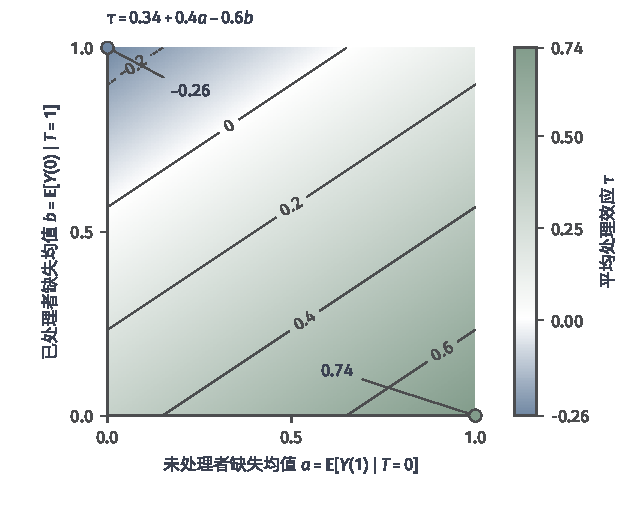
\includegraphics[width=105mm]{figures/00-shared/mathematical-preliminaries-lower/01-random-variables-distributions-and-causality/matplotlib/causal-manski-missing-outcome-geometry/figure.pdf}
  \caption{两个缺失潜在结果均值生成的Manski锐界。固定\(P(T=1)=0.6\)、已处理组观察均值\(0.7\)、未处理组观察均值\(0.2\)，并且只要求一致性及\(0\leq Y(t)\leq1\)。横、纵轴为两类缺失均值\(a,b\)，方形内全部赋值均与这些观测相容；色阶和等高线表示\(\tau=0.34+0.4a-0.6b\)。两个角点达到\(-0.26\)与\(0.74\)，范围宽度为\(1\)。色阶反映相容机制的目标差异，不是抽样误差。}
  \label{fig:causal-manski-missing-outcome-geometry}
\end{figure}

\subsubsection{支持缺口下的效应与策略界}
\label{sec:causal-support-policy-bounds}

现在假设条件交换性可信，但双侧重叠只在协变量区域\(\mathcal O\)成立。用
\(\mathcal N\)表示目标总体中缺少某种处理的区域，两者不交且覆盖目标总体。
结果仍在\([0,1]\)时，条件效应\(\tau(x)\in[-1,1]\)，故
\[
  \tau=
  \mathbb E[\tau(X)\mathbb I\{X\in\mathcal O\}]
  +\mathbb E[\tau(X)\mathbb I\{X\in\mathcal N\}].
\]
第一项由调整式识别，第二项只能先按范围控制，得到
\begin{equation}
  \begin{aligned}
    &\mathbb E[\tau(X)\mathbb I\{X\in\mathcal O\}]
      -\mathbb P(X\in\mathcal N)\leq\tau\\
    &\qquad\leq
      \mathbb E[\tau(X)\mathbb I\{X\in\mathcal O\}]
      +\mathbb P(X\in\mathcal N).
  \end{aligned}
  \label{eq:causal-overlap-gap-bounds}
\end{equation}
这是一组有效界，未声称总是锐界；缺口区域中若仍观察到一种处理的结果，
利用这一侧均值还可能收紧。限制目标人群到\(\mathcal O\)可以点识别重叠人群效应，
但已经改变了目标总体。假设缺口内效应与邻近区域平滑、同号或落在更小范围，也能
收紧答案，却都是额外外推条件，不能由已覆盖部分的拟合优度证明。

单步策略评价需要的支持可以更少。沿用式~\eqref{eq:causal-policy-value}的有限
动作集合及目标策略\(\pi\)，其中\(a\)仍表示将同一个\(T\)设为值\(a\)的行动。
记录自然处理选择的资料称为日志，记其中的动作概率为
\(e_a(x)=\mathbb P(T=a\mid X=x)\)。假设对所有动作，
\(L\leq Y(a)\leq H\)，且一致性和给定\(X\)的交换性成立。若目标覆盖条件为
\[
  \pi(a\mid x)>0\quad\Longrightarrow\quad e_a(x)>0
\]
并在目标总体中几乎处处成立，则
\[
  \begin{aligned}
    \mathbb E\left[\frac{\pi(T\mid X)}{e_T(X)}Y\middle|X\right]
    &=
    \sum_{\substack{a\in\mathcal A\\e_a(X)>0}}
      e_a(X)\frac{\pi(a\mid X)}{e_a(X)}
      \mathbb E[Y\mid T=a,X]\\
    &=
    \sum_{a\in\mathcal A}\pi(a\mid X)\mathbb E[Y(a)\mid X].
  \end{aligned}
\]
对\(X\)取期望，得到
\begin{equation}
  V(\pi)=\mathbb E\left[\frac{\pi(T\mid X)}{e_T(X)}Y\right].
  \label{eq:causal-policy-value-weighting}
\end{equation}
这是换测度（用密度比把一个分布下的期望改写为另一个分布下的加权期望）的一个因果用途：改变动作分配，
保留给定背景与动作的结果机制。权重只在日志实际可能选择的动作上求值，
覆盖条件使其余动作的目标概率为零，无须引入\(0/0\)约定。

覆盖失败时，记目标策略落入缺口的概率质量及已识别贡献为
\[
  \begin{aligned}
    r&=\mathbb E_X\left[\sum_{a:e_a(X)=0}\pi(a\mid X)\right],\\
    K&=\mathbb E_X\left[
      \sum_{a:e_a(X)>0}\pi(a\mid X)\mathbb E[Y\mid T=a,X]
    \right].
  \end{aligned}
\]
缺口部分的贡献在\([Lr,Hr]\)内，因而
\begin{equation}
  K+Lr\leq V(\pi)\leq K+Hr.
  \label{eq:causal-policy-value-bounds}
\end{equation}
两个策略的价值范围若完全分离，就能确定排序；若重叠，单独看边际范围未必能
判断。它们使用同一组未知潜在结果，不能把各自端点当作独立可选。
例如两策略完全相同时，无论各自的价值范围多宽，价值差都严格为零。
一般应对
\[
  V(\pi_1)-V(\pi_2)
  =
  \mathbb E_X\sum_a
    \bigl(\pi_1(a\mid X)-\pi_2(a\mid X)\bigr)\mathbb E[Y(a)\mid X]
\]
直接构造联合识别集合或上下界。拟合器对缺口给出的单一外推，不是额外的排序证据。

图~\ref{fig:causal-confounding-coverage}把混杂与覆盖分别数值化。左图回顾前面的
风险分层例子；右图另设结果范围为\([0,1]\)，已覆盖部分条件平均收益为\(0.6\)，
故\(K=0.6(1-r)\)。在\(r=0.2\)时，价值范围为\([0.48,0.68]\)。
宽度\(0.2\)来自缺口中的未知结果机制，不会因增加同一覆盖区域内的样本而消失。
\begin{figure*}[htbp]
  \centering
  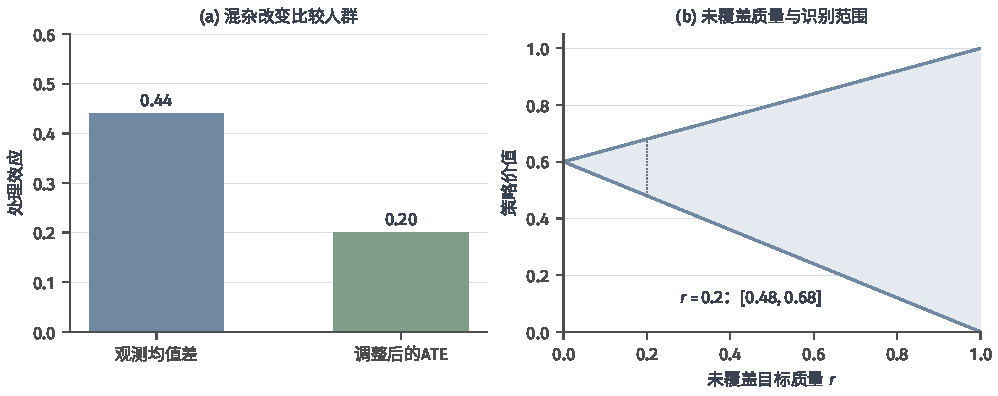
\includegraphics[width=\linewidth]{figures/00-shared/mathematical-preliminaries-lower/01-random-variables-distributions-and-causality/matplotlib/causal-confounding-coverage/figure.pdf}
  \caption{两个独立的教学构造。左图比较风险分层例子的观测均值差\(0.44\)与调整
  效应\(0.20\)。右图按式~\eqref{eq:causal-policy-value-bounds}绘制
  \([0.6(1-r),0.6(1-r)+r]\)。阴影为总体识别范围，不是抽样置信带；
  两个面板不表示同一数据集。}
  \label{fig:causal-confounding-coverage}
\end{figure*}

这里的策略只作一次行动。\BookSectionRef{sec:decision-dynamic-programming}{第~\ref{sec:decision-dynamic-programming}节}建立序贯
策略后，必须逐时检查历史覆盖、时间变化的混杂及轨迹结果定义，不能把单步权重
直接套到整条轨迹。

\subsubsection{未观测混杂下的敏感性范围}
\label{sec:causal-sensitivity-ranges}

另一种缺口不是某类记录完全没有，而是相同已观测背景下仍存在未观测选择差异。
敏感性分析不强行断言该差异为零，而是规定其允许强度，检查结论随强度怎样变化。

先用一个最小线性模型定位偏差。设变量中心化，
\[
  T=\alpha U+\varepsilon_T,\qquad
  Y=\beta T+\gamma U+\varepsilon_Y,
\]
其中\(U,\varepsilon_T,\varepsilon_Y\)两两独立、方差有限，且
\(\operatorname{Var}(T)>0\)。理想设定\(T=t\)时，固定背景的结果对\(t\)的
导数为\(\beta\)。但只将\(Y\)对自然处理\(T\)作总体线性回归，得到
\begin{equation}
  \begin{aligned}
    \beta_{\mathrm{obs}}
    &=\frac{\operatorname{Cov}(T,Y)}{\operatorname{Var}(T)}\\
    &=\beta+
      \gamma\frac{\alpha\operatorname{Var}(U)}{\operatorname{Var}(T)}.
  \end{aligned}
  \label{eq:causal-linear-confounding-bias}
\end{equation}
这里用到了
\(\operatorname{Cov}(T,Y)=\beta\operatorname{Var}(T)
+\gamma\operatorname{Cov}(T,U)\)，以及
\(\operatorname{Cov}(T,U)=\alpha\operatorname{Var}(U)\)。
共同背景同时进入处理与结果，产生了第二项。这里的\(\beta_{\mathrm{obs}}\)最小化总体均方线性预测误差，是一个常数；条件均值\(t\mapsto\mathbb E[Y\mid T=t]\)则未必为直线。
例如取\(\alpha=\gamma=1,\beta=0\)，令\(U\)等概率取\(\pm1\)、\(\varepsilon_T\sim\mathcal N(0,1)\)与\(U\)独立，且\(\varepsilon_Y=0\)。此时\(Y=U\)，两种背景的条件概率比为\(e^{2t}\)，故
\[
 \mathbb E[Y\mid T=t]=\tanh t,\qquad
 \left.\frac{\mathrm d}{\mathrm dt}\mathbb E[Y\mid T=t]\right|_{t=0}=1,
 \qquad\beta_{\mathrm{obs}}=\frac12.
\]
因此线性投影偏差不能不加条件地当作每个剂量点的导数偏差。若只知道线性投影偏差\(\beta_{\mathrm{obs}}-\beta\)的绝对值不超过
\(\Lambda\)，则
\(\beta\in[\beta_{\mathrm{obs}}-\Lambda,\beta_{\mathrm{obs}}+\Lambda]\)。
观测可以估计\(\beta_{\mathrm{obs}}\)，却不能在没有额外信息时把
\(\alpha,\gamma,\beta\)各自分开；改变函数形式也会改变敏感性参数的含义。

异质或非线性响应不一定有一个统一斜率修正量。仍记
\(\mu_t(x)=\mathbb E[Y\mid T=t,X=x]\)和\(e(x)=\mathbb P(T=1\mid X=x)\)。
在\(0<e(x)<1\)且相关条件期望有限时，定义选择偏差函数
\[
  \begin{aligned}
    b_1(x)&=\mathbb E[Y(1)\mid T=1,X=x]
            -\mathbb E[Y(1)\mid T=0,X=x],\\
    b_0(x)&=\mathbb E[Y(0)\mid T=1,X=x]
            -\mathbb E[Y(0)\mid T=0,X=x].
  \end{aligned}
\]
条件交换性蕴含\(b_1=b_0=0\)，但反过来只得到条件均值交换性，
不能推出完整潜在结果分布相同。比如两组都均值为零，一组恒等于零，另一组等概率
取\(1,-1\)，均值相同仍保留分布差异。

一致性给出
\(\mathbb E[Y(1)\mid T=1,X=x]=\mu_1(x)\)，再由全期望
\[
  \begin{aligned}
    \mathbb E[Y(1)\mid X=x]
    &=e(x)\mu_1(x)+(1-e(x))(\mu_1(x)-b_1(x))\\
    &=\mu_1(x)-(1-e(x))b_1(x).
  \end{aligned}
\]
另一侧有
\[
  \begin{aligned}
    \mathbb E[Y(0)\mid X=x]
    &=(1-e(x))\mu_0(x)+e(x)(\mu_0(x)+b_0(x))\\
    &=\mu_0(x)+e(x)b_0(x).
  \end{aligned}
\]
相减得到
\begin{equation}
  \tau(x)=\mu_1(x)-\mu_0(x)
  -(1-e(x))b_1(x)-e(x)b_0(x).
  \label{eq:causal-selection-bias-function}
\end{equation}
若领域知识仅支持
\(|b_1(x)|\leq\Gamma_1(x)\)及\(|b_0(x)|\leq\Gamma_0(x)\)，三角不等式给出
\begin{equation}
  \begin{aligned}
    \mu_1(x)-\mu_0(x)-\Delta(x)
    &\leq\tau(x)\\
    &\leq\mu_1(x)-\mu_0(x)+\Delta(x),
  \end{aligned}
  \label{eq:causal-sensitivity-bounds}
\end{equation}
其中\(\Delta(x)=(1-e(x))\Gamma_1(x)+e(x)\Gamma_0(x)\)。
重叠在目标总体几乎处处成立、潜在结果及相应控制量可积时，再对\(X\)平均便得到
ATE范围。该范围是当前偏差约束的有效包络；若还有限定结果范围或其他联合约束，
不能未经可达性检查就宣称它为锐界。

代入数值可以看清偏差约束如何影响结论。以下均值、效应与偏差均使用\(Y\)的同一
计量单位，沿用本小节的一般实值结果设定。取某个协变量分层上
\(e(x)=0.3\)、\(\mu_1(x)-\mu_0(x)=0.5\)，
并设偏差仅满足\(\Gamma_1(x)=0.2\)、\(\Gamma_0(x)=0.1\)，则
\(\Delta(x)=0.7\times0.2+0.3\times0.1=0.17\)，效应区间为
\([0.33,0.67]\)。两项的权重并不相同：\(b_1\)以\(1-e(x)\)加权，\(b_0\)以
\(e(x)\)加权。前一项修正未处理者缺失的\(Y(1)\)，后一项修正已处理者缺失的
\(Y(0)\)；若其他量固定而\(e(x)\)增大，前一项的权重减小，后一项的权重增大。

先保持\(e(x)=0.3\)及观测均值差\(0.5\)不变，只把两个偏差上界都放宽到
\(0.5\)个结果单位。此时\(\Delta(x)=0.7\times0.5+0.3\times0.5=0.5\)，效应
包络为\([0,1]\)，已经包含零；当前偏差约束不足以确定效应严格为正。这是效应的
包络，并未另外假定结果\(Y\)只能取\([0,1]\)中的值。

再恢复最初的\(\Gamma_1(x)=0.2\)、\(\Gamma_0(x)=0.1\)，保持观测均值差
\(0.5\)，仅把\(e(x)\)从\(0.3\)改为\(0.8\)，便有
\[
  \Delta(x)=0.2\times0.2+0.8\times0.1=0.12,
  \qquad \tau(x)\in[0.38,0.62].
\]
这里更大的权重移向了较小的\(\Gamma_0\)，所以包络比最初的\([0.33,0.67]\)窄；
处理比例更极端本身并不保证包络缩小，若两个上界都仍为\(0.5\)，则
\(\Delta(x)\)仍是\(0.5\)。这些比较把结论与所许偏差的门槛联系起来：本例观测
差为正，要使效应下界严格大于零，需有\(\Delta(x)<0.5\)。

为了连续比较同一类偏差假设，可固定\(e(x)=0.3\)和观测均值差\(0.5\)，令
\(\Gamma_1(x)=0.2s\)、\(\Gamma_0(x)=0.1s\)，其中\(s\geq0\)是共同放宽倍数。
于是\(\Delta(x)=0.17s\)，图~\ref{fig:causal-sensitivity-effect-envelope}中的下界在
\(s=0.5/0.17=50/17\)处恰好达到零。图中带状范围表达未观测偏差假设允许的效应包络，
不是由重复抽样得到的置信带；\(s\)也不是样本量。

\begin{figure}[htbp]
  \centering
  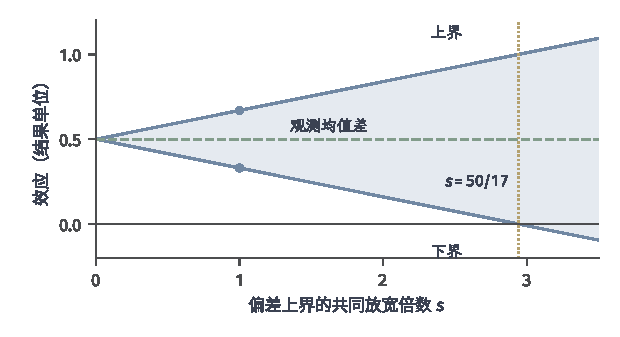
\includegraphics[width=105mm]{figures/00-shared/mathematical-preliminaries-lower/01-random-variables-distributions-and-causality/matplotlib/causal-sensitivity-effect-envelope/figure.pdf}
  \caption{选择偏差上界放宽时的效应包络。固定一个协变量分层及\(e(x)=0.3\)、\(\mu_1(x)-\mu_0(x)=0.5\)，令\(\Gamma_1=0.2s\)、\(\Gamma_0=0.1s\)。蓝线与浅蓝区域为\([0.5-0.17s,0.5+0.17s]\)，绿虚线为固定的观测均值差；\(s=1\)的两个点标出\([0.33,0.67]\)，黄竖线标出下界达到零的门槛。所有纵轴量使用相同结果单位，图中未另外约束结果只能取\([0,1]\)。}
  \label{fig:causal-sensitivity-effect-envelope}
\end{figure}

\(\Gamma_t\)是关于未观测差异的假设，不是样本自动生成的误差条。报告应展示在多大
强度下结论变号或越过决策阈值，而不只给一个恰好保留原结论的值。
其他有根据的假设也能缩小相容类。例如个体\term{单调性}（monotonicity）
\[
  Y(1)\geq Y(0)\quad\text{几乎必然}
\]
排除所有受损个体，故在加入单调性后的相容类非空时，ATE至少为零。
若已有有效范围\([L_{\mathrm{old}},U_{\mathrm{old}}]\)，应将它与\([0,+\infty)\)相交，
得到\([\max\{L_{\mathrm{old}},0\},U_{\mathrm{old}}]\)，而不是把正的已有下界降为零。
交集为空意味着单调性与当前观测或已有假设冲突，不能把空范围当成效应结论。
它比“平均有益”更强。若已知个体效应位于\([-\rho,\rho]\)，支持缺口中的
\([-1,1]\)可换成更窄范围；平滑外推也必须作为新增机制限制声明。

跨环境资料可以提供另一种约束。若源环境有随机试验，目标环境给出协变量分布，
并假设条件效应在两环境相同，且目标协变量分布对源环境分布绝对连续，即源环境
的零概率背景集在目标环境中也为零概率。再假设目标环境的两种潜在结果可积，
则相同的条件效应在目标协变量分布下也可积，并有
\[
  \tau_{\mathrm{target}}
  =\int\tau_{\mathrm{source}}(x)\,P_{X,\mathrm{target}}(\mathrm dx).
\]
这是条件效应稳定和目标覆盖共同给出的运输关系；在离散情形，覆盖要求目标中
出现的背景在源环境也有正概率。连续情形仅有拓扑支持包含还不够，应使用上述
绝对连续条件。条件效应稳定与目标覆盖条件都不能由稳定预测关联自动推出。
共同隐藏原因、选择过程或多个机制同步变化都可能产生稳定关联。

相容类也可用于第~\ref{sec:causal-counterfactual-recourse}节的反事实、补救与公平
目标。跨世界配对不同的模型可能同样解释试验边缘，却改变行动成功概率或公平判断。
此时应传播这些模型差异，而不是仅报告选定生成模型内的模拟精度。

\subsection{有限样本下的响应估计}
\label{sec:causal-response-estimation}

即使识别式成立，条件响应、处理概率与总体权重通常仍需从样本估计。比如调整法用
\(\widehat\mu_t\)代替\(\mu_t\)，再在目标背景样本上平均：
\[
  \widehat\tau
  =\frac1n\sum_{i=1}^n
    \bigl(\widehat\mu_1(X_i)-\widehat\mu_0(X_i)\bigr).
\]
这只是识别式的一种代入估计，不自动具有无偏性或某种收敛速度。拟合误差、目标样本
的抽样误差以及重复使用同一数据引入的依赖，仍须按第~\ref{sec:rv-inference}节
的估计与数据复用规则分析。采用样本拆分或交叉拟合时，应明确哪些样本拟合、哪些
样本评价，以及相应误差条件。

逆概率法还要估计倾向概率。很小但非零的真实概率允许总体识别，却可能使估计方差
很大；截断权重可改变偏差与方差，但不能被解释为凭空补足支持。更灵活的拟合器
或交叉拟合同样不能修复交换性错误。

部分识别时，估计对象可以是识别集合的端点或其外包络。识别集合在总体分布已知时
仍可能不是单点，表达机制歧义；\term{置信区间}来自有限样本，表达总体目标、
识别集合或端点的估计误差。对端点构造置信范围，还需按所用统计方法处理两个端点
共同的覆盖要求，不能把端点估计直接当作已知真界。

实际报告应分别列出相容机制留下的范围、抽样造成的不确定性，以及积分或优化中的
数值误差。增加样本主要改善第二项，改善算法主要影响第三项；改变设计、扩大目标
行动覆盖或加入可辩护的机制限制，才可能缩小第一项。尤其在效应符号或行动阈值附近，
应同时报告对支持处理、敏感性参数及目标总体选择的依赖。

\section{因果生成结构的表示}
\label{sec:causal-generating-structure}

培训可以先改变技能，技能再改变成绩，这类“一步步如何产生”的过程很难只用一个整体映射看清。更自然的写法是为每个变量单独给出一条局部生成规则：培训由个人情况决定，技能由培训和天赋决定，成绩由培训、技能和其他因素决定。把这些局部规则合起来，就能构造此前使用的整体响应映射。每条局部方程规定怎样产生一个变量，背景的联合分布规定未展开因素怎样共同变化，图则记录方程读取哪些变量。只有把这三项结合，才能计算替换处理规则后应沿哪些关系重新求值。

\subsection{局部机制的结构方程表示}
\label{sec:causal-local-structural-equations}

把模型内需要解释的变量称为内生变量，把当前模型不再解释的背景称为外生变量。
“外生”是相对于模型边界而言，并不意味着这些量在现实中没有原因，也不自动意味着
它们彼此独立。进入某个变量生成函数的其他内生变量称为它的父变量，表示该局部机制
直接读取哪些输入。

这些局部方程为什么要求“无环”？因为我们希望给定背景后，每个变量都能被一步步算出来，而不是陷入“甲依赖乙、乙又依赖甲”的循环。有环时方程可能无解或有无穷多解（本章末会给出例子），干预之后也无法确定该按什么次序重新求值。无环结构保证存在一个求值次序，使每个变量被计算时它所依赖的变量都已经算好。
\begin{definition}[无环结构因果模型]
  \label{def:causal-structural-model}
  本章的\term{结构因果模型}（structural causal model, SCM）由内生变量
  \(\bm V=(V_1,\ldots,V_d)\)的可测状态空间、外生背景
  \(\bm U=(U_1,\ldots,U_d)\)的联合分布及可测结构函数组成：
  \begin{equation}
    V_j=f_j(\operatorname{pa}_j,U_j),
    \qquad j=1,\ldots,d.
    \label{eq:causal-scm-definition}
  \end{equation}
  其中\(\operatorname{pa}_j\)收集进入第\(j\)个函数的其他内生变量。
  \term{无环}（acyclic）要求存在节点次序\(j_1,\ldots,j_d\)，使每个函数的
  内生输入都来自次序中更早的节点。外生分量可以相关。
\end{definition}

把每个内生变量画成节点，在\(V_k\)作为输入进入\(f_j\)时画箭头\(V_k\to V_j\)，
便得到有向无环图，简称DAG。上述求值次序已足以理解无环性，不需要先学习图排序
算法。SCM的箭头具有生成语义；若箭头只用于表示联合分布的条件分解，就不能据此
判断改变输入的后果\scite{math-pearl2009causality}

例如，培训\(T\)、技能\(M\)和成绩\(Y\)可以写成
\[
  T=f_T(U_T),\qquad
  M=\alpha T+U_M,\qquad
  Y=\beta T+\gamma M+U_Y.
\]
这里的直接输入关系为\(T\to M\)、\(T\to Y\)、\(M\to Y\)。若
\(U_T,U_M,U_Y\)相关，处理选择还可能与技能或成绩背景相联系；仅画出这三条内生边
不足以表示全部共同背景。要使用独立噪声DAG的概率规则，必须另行要求这些背景独立，
或把相关性的共同来源显式放进模型。

有限维模型可以把局部函数写成\(f_{j,\bm\theta_j}\)，并用
\(\bm\theta=(\bm\theta_1,\ldots,\bm\theta_d)\)汇集参数。上例的
\(\alpha,\beta,\gamma\)是局部作用参数；一般SCM则不必属于有限维函数族。
指定关系但不知道函数，或拟合函数却没有确定它的因果语义，都仍留下结构上的未知。

\subsection{局部机制的复合与响应生成}
\label{sec:causal-mechanism-composition}

有了局部方程，定义~\ref{def:causal-response-interface}假定的自然映射就可以
实际构造。无环次序让每一步只读取已经得到的值，因此既给出计算过程，也排除了
同一背景下出现多个自然解的歧义。

\begin{theorem}[无环机制的唯一可测响应]
  \label{thm:causal-acyclic-response}
  对定义~\ref{def:causal-structural-model}中的模型，每个背景
  \(\bm u\)唯一确定一组满足所有结构方程的内生取值。
  所得自然映射\(F_M:\mathcal U\to\mathcal V\)可测。将任意指定的一组方程
  替换为常量方程后，所得映射\(F_M^a\)同样存在、唯一且可测。
  对单变量理想干预，响应\((t,\bm u)\mapsto R_M(t,\bm u)\)联合可测。
\end{theorem}
\begin{proof}
  取符合无环性的次序\(j_1,\ldots,j_d\)。第一个变量没有内生父变量，
  因而\(v_{j_1}=f_{j_1}(u_{j_1})\)唯一确定，且是\(\bm u\)的可测函数。
  假设前\(k-1\)个变量已唯一确定为可测函数。第\(k\)个方程的父变量都在其中，
  将这些函数及\(u_{j_k}\)代入可测的\(f_{j_k}\)，便得到唯一且可测的
  \(v_{j_k}\)。归纳到\(d\)，得到满足全部方程的可测向量\(F_M(\bm u)\)。
  任何另一组解在第一个坐标都必须相同；逐坐标应用同一理由，便证明唯一性。

  常量替换只删除输入，不增加逆向依赖，原次序仍可使用。被替换坐标直接取行动
  指定值，其余坐标按同样归纳求出，从而得到\(F_M^a\)。
  若把处理值\(t\)也作为输入，被替换坐标是乘积空间上的投影
  \((t,\bm u)\mapsto t\)，其余步骤仍是可测函数的复合，因此
  \(F_M^{a(t)}(\bm u)\)及其结果坐标\(R_M(t,\bm u)\)联合可测。
\end{proof}

自然分布是\((F_M)_{\#}P_{\bm U}\)，干预分布是
\((F_M^a)_{\#}P_{\bm U}\)。两个推前共用同一个背景分布，只改变生成映射。
若理想干预值恰好等于该背景下的自然处理值，那么自然解也满足替换后的全部方程；
由唯一性，两组解相同。这也证明了这种构造中的一致性，而不只是另行假定
\(Y=Y(T)\)。

若结果方程为\(Y=f_Y(T,X,U_Y)\)，且\(X\)不受处理干预影响，则
\begin{equation}
  Y(t)=f_Y(t,X,U_Y).
  \label{eq:causal-scm-potential-outcome}
\end{equation}
因此\(\mathcal L(Y(t))=\mathcal L(Y\mid\operatorname{do}(T=t))\)。
若结果还依赖处理会改变的技能\(M\)，则必须先重算\(M(t)\)，不能仍代入事实技能。
对上面的线性机制，
\[
  M(t)=\alpha t+U_M,\qquad
  Y(t)=(\beta+\gamma\alpha)t+\gamma U_M+U_Y,
\]
所以整体响应导数为\(\beta+\gamma\alpha\)，不只是局部结果方程中固定\(M\)
时的偏导数\(\beta\)。取\(\alpha=2,\beta=1,\gamma=3\)，增加一单位培训使成绩
增加\(7\)，其中直接贡献为\(1\)，经技能传递的贡献为\(6\)。
对可微的非线性机制\(M=f_M(T,U_M)\)、\(Y=f_Y(T,M,U_Y)\)，链式法则给出
\[
  \frac{\partial R_M(t,\bm u)}{\partial t}
  =
  \frac{\partial f_Y}{\partial t}
  +
  \frac{\partial f_Y}{\partial m}
  \frac{\partial f_M}{\partial t},
\]
各偏导数均在该背景的干预取值处计算。这连接了第~\ref{sec:causal-local-response}节
的整体局部变化与本节的局部方程；对它再作总体平均，仍须检查导数与积分交换条件。

图~\ref{fig:causal-direct-mediated-total-response}沿用\(\alpha=2,\beta=1,\gamma=3\)，再固定背景\(U_M=U_Y=0\)，将“保留技能方程”和“固定技能值”分开计算。只设置培训\(T=t\)时，原技能规则仍要读取新的处理值，所以\(M(t)=2t\)，总成绩为\(Y(t)=t+3(2t)=7t\)。若另加一项把技能同时固定为\(0\)的联合干预\(\operatorname{do}(T=t,M=0)\)，成绩才变成\(t\)。右图把从\(t=0\)到\(1\)的增量分成直接的\(1\)与经技能传递的\(3\times2=6\)：去掉后者改变了行动目标，不能仍把剩下的\(1\)称为只改变培训的总响应。

\begin{figure*}[htbp]
  \centering
  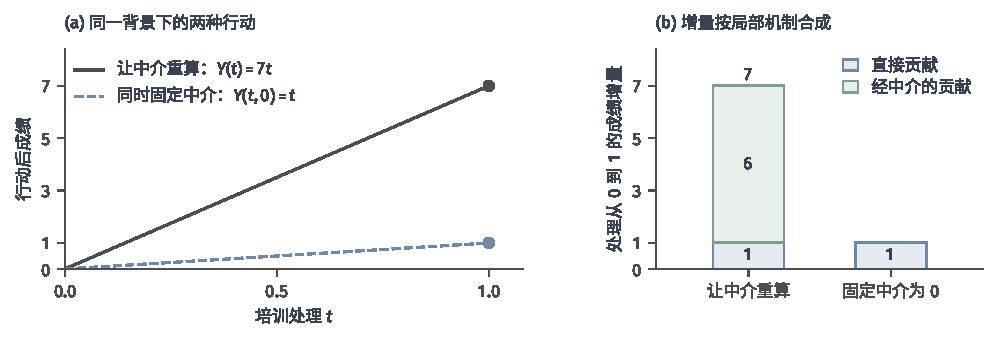
\includegraphics[width=169mm]{figures/00-shared/mathematical-preliminaries-lower/01-random-variables-distributions-and-causality/matplotlib/causal-direct-mediated-total-response/figure.pdf}
  \caption{局部规则的复合与总响应。教学机制为\(M=2T+U_M\)、\(Y=T+3M+U_Y\)，背景固定为\(U_M=U_Y=0\)。左图灰实线只设置\(T=t\)，让技能按原方程重算；蓝虚线同时设置\(T=t,M=0\)，图中以\(Y(t,0)\)表示这一联合干预结果。右图比较两种行动从\(t=0\)到\(1\)的成绩增量，蓝色为直接贡献\(1\)，绿色为经技能传递的贡献\(6\)。曲线与柱高来自同一给定线性机制，不是观测回归系数，也不建立一般中介效应的识别结论。}
  \label{fig:causal-direct-mediated-total-response}
\end{figure*}

\begin{example}[计算模型中的受控替换]
  \label{ex:causal-controlled-computation}
  一套参数已经固定的程序先计算中间读数，再把这个读数与其他输入合成输出。
  我们希望检查输出是否依赖实际读到的内容，因而把程序本身作为此次研究的生成机制，
  指定哪些计算保持原样、在哪一步替换数值。这个问题与推断程序外部的现实机制不同。

  设输入为\(\bm x\in\mathbb R^d\)，保留条件为\(\bm c\in\mathbb R^r\)，
  中间读数为\(\bm h\in\mathbb R^k\)，标量输出为\(\widehat y\)。固定参数
  \(\bm\theta\)以后，原程序为
  \[
    \bm h=f_{\bm\theta}(\bm x,\bm c),\qquad
    \widehat y=g_{\bm\theta}(\bm x,\bm h,\bm c).
  \]
  \(\bm c\)收集此次比较保留的其他输入和已有历史；这里先假定计算是确定性的。
  若程序含随机计算，还须固定两次运行所用的外生随机数，或另行声明对哪些随机量取平均。

  检查某次读取的作用时，保持\(\bm x,\bm c,\bm\theta\)不变，只在程序实际消费
  \(\bm h\)的位置把它换为同维且程序可接受的值\(\bm v\)，并沿原有规则重算所有受影响的后继量。
  替换后的输出与原输出之差为
  \begin{equation}
    \Delta_{\mathrm{read}}(\bm v;\bm x,\bm c)
    =g_{\bm\theta}(\bm x,\bm v,\bm c)
    -g_{\bm\theta}\bigl(\bm x,f_{\bm\theta}(\bm x,\bm c),\bm c\bigr).
    \label{eq:causal-computational-read-replacement}
  \end{equation}
  这就是把读数方程替换为\(\bm h=\bm v\)所产生的程序响应。若一次读取还涉及
  替换之前已经确定的条目选择、读取位置或读取权重，而目标只比较被消费的内容，这些量也须保持原样；
  同时改变它们得到的是另一项干预。

  若改的是输入记录\(\bm x\mapsto\bm x'\)，中间读数也应按原规则重新计算，得到
  \[
    \widehat y_{\mathrm{input}}(\bm x';\bm c)
    =g_{\bm\theta}\bigl(\bm x',f_{\bm\theta}(\bm x',\bm c),\bm c\bigr).
  \]
  把输入改为\(\bm x'\)却保留原读数，对应同时设置输入和读数，通常不等于这项
  输入替换。删除整个模块、改变参数或重新训练又会替换更多规则，回答的也不是同一问题。

  只要替换值在程序接受的定义域内，以上响应就能通过运行程序求出。
  替换值即使偏离训练分布，也不自动使程序响应失去定义；但这次响应不能直接概括
  训练分布内其他输入上的内容依赖，更不能单凭它推断现实中的因果效应。
  要回答现实变量改变后结果会怎样，还须说明程序输入怎样对应现实变量、行动会改变
  哪些后继因素，以及固定的计算规则是否仍能代表这些因素的生成机制。
  因而，受控替换直接支持的是指定程序、指定位置和指定替换下的输出比较；
  从这一比较到现实行动的效果，仍需本章前面讨论的机制假设与识别依据。
\end{example}

回到结构因果模型，在外生噪声相互独立时，还可以用局部概率核表达同一生成计算。记
\[
  K_j(B\mid\bm v_{\operatorname{pa}_j})
  =
  \mathbb P\bigl(f_j(\bm v_{\operatorname{pa}_j},U_j)\in B\bigr).
\]
每个核都由机制及噪声分布指定，沿无环次序复合这些核便得到联合分布。独立性保证
当前噪声不会被已经生成的变量额外筛选。若每个局部核相对于固定的坐标参考测度
\(\mu_j\)都有可测密度，联合参考测度取\(\bigotimes_j\mu_j\)，则
\[
  p(\bm v)=\prod_{j=1}^d p(v_j\mid\operatorname{pa}_j).
\]
离散坐标可取计数测度，相应密度就是质量函数。不满足这种支配条件时，
仍用概率核的复合与积分表达联合规律。
在上述受支配情形中，理想干预把处理核换成点质量，其余核保持原样，于是得到\term{截断分解}
\begin{equation}
  p(\bm v_{-T}\mid\operatorname{do}(T=t))
  =
  \prod_{j:V_j\ne T}
  p(v_j\mid\operatorname{pa}_j)\big|_{T=t}.
  \label{eq:causal-truncated-factorization}
\end{equation}
这里\(\bm v_{-T}\)表示删除处理坐标后的变量集合。公式来自机制替换，不是对
任意概率分解删除一个因子都能得到因果分布。外生噪声相关时，上述独立核复合一般
不成立；应回到完整背景的推前，或显式展开相关来源。

局部因子必须使用结构机制指定的版本。观测分布只在父变量实际出现的支持上确定
条件分布；干预若产生了未见过的父变量组合，机制可以给出答案，但资料未必能识别
该答案。随意补一个支持外的条件密度，不会把模型外推变成数据结论。

对简单结构\(X\to T\)、\(X\to Y\)、\(T\to Y\)，用独立的新随机量按
\(q(t\mid x)\)分配处理，并保持其余独立噪声机制不变。
在上述共同参考测度下，若新处理核也具有密度\(q\)，得到
\begin{equation}
  p^q(x,t,y)=p(x)q(t\mid x)p(y\mid t,x).
  \label{eq:causal-stochastic-intervention}
\end{equation}
这正是第~\ref{sec:causal-intervention-potential-outcomes}节随机干预构造的局部
表达。确定性策略用点质量核表示，不必假装它有通常的Lebesgue密度。
策略若同时改变参与人群、结果测量或其他机制，就不能只替换处理因子。
更一般的机制替换也需要保证修改后的方程有明确解；添加依赖关系时，原无环次序
可能不再适用。

循环方程说明这一边界并非形式问题。例如\(V_1=V_2+1,V_2=V_1\)无解，而
\(V_1=V_2,V_2=V_1\)有无穷多组解。反馈系统可能需要动态演化、平衡选择或额外
唯一性条件，不能直接套用本节递归证明。

\subsection{变量关系的图表示与调整条件}
\label{sec:causal-graph-adjustment}

给定结构函数以后，逐个代入就能生成干预响应。选择调整变量时却未必需要知道每个函数的具体形式：我们要判断哪些处理前背景足以阻断处理选择与结果之间的联系。图只保留局部方程的输入关系，将满足同一结构的机制放在一起考察。局部路径说明条件化为何可能消除或制造联系；全图检查再判断是否还留有其他路径，后门准则据此为前面的调整公式提供充分条件。

\subsubsection{局部因果关系与调整影响}
\label{sec:causal-local-path-patterns}

结构\(T\leftarrow X\to Y\)把\(X\)称为\(T\)与\(Y\)的
\term{共同原因}（common cause）。即使处理并不影响结果，不同\(X\)人群接受
处理的比例不同，也会使\(T,Y\)在自然记录中相关。这是混杂产生的一种方式。
第~\ref{sec:causal-adjustment-identification}节的风险分层算例正是通过在同一背景层
比较，再用同一目标权重平均，消除了由两组构成不同造成的差异。

结构\(T\to M\to Y\)中的\(M\)是\term{中介变量}（mediator）：处理对结果的
一部分影响经过它传递。若目标是总效应，固定\(M\)会阻断这部分变化；若研究同时
设定\(T=t,M=m\)的响应，则需明确这是不同的联合干预。
在线性例子中，固定中介后的处理系数为\(\beta\)，让中介随处理变化的总系数为
\(\beta+\gamma\alpha\)。这并不建立一般路径效应的识别公式，只说明两种目标不同。

结构\(T\to C\leftarrow Y\)中的\(C\)是\term{碰撞点}（collider），两条箭头
在此相遇，形象地说就是两条因果链“对撞”到同一个变量上。不以\(C\)筛选时，这条路径本身不要求两端相关；一旦给定\(C\)（按它分层、只看某个子群，或用它做选择），却可能
引入关联。这是三种结构里最反直觉的一种，值得用例子记住。例如两个独立能力共同决定总分，入选要求总分超过阈值且两项能力可以
补偿，那么入选者中一项能力较弱的人往往需要另一项更强——两项本来独立的能力，在“已入选”这个子群里变成了负相关。若入选规则改成两项能力
分别超过各自阈值，这种负关联未必出现。关系的方向取决于选择机制，不能把选择
后的相关解释为一种能力造成另一种能力。

图~\ref{fig:causal-local-path-patterns}用双边框标记已经给定的中间变量。共同原因和中介在所画路径上都是非碰撞点，给定它们会关闭该路径；给定碰撞点则会打开原本关闭的路径，但路径活跃并不保证实际分布一定存在非零统计依赖。调整变量的作用因而取决于它在路径中的角色。较大图还可能有多条连接同一对变量的路径，关闭一个局部片段后须继续检查其他路径。
\begin{figure*}[htbp]
  \centering
  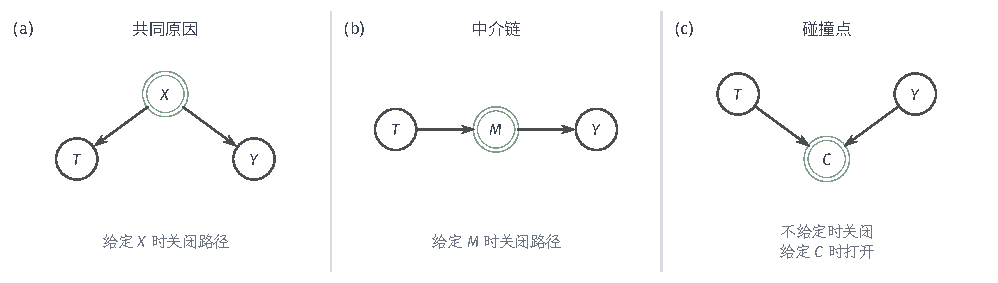
\includegraphics[width=\linewidth]{figures/00-shared/mathematical-preliminaries-lower/01-random-variables-distributions-and-causality/tikz/causal-local-path-patterns/figure.pdf}
  \caption{共同原因、中介与碰撞点的局部路径。双边框表示节点已加入条件集。
  共同原因和中介是非碰撞点，给定后关闭这条路径；给定碰撞点则打开原本关闭的
  路径。路径打开表示图不再保证相应独立性，并不指定相关的大小或正负。}
  \label{fig:causal-local-path-patterns}
\end{figure*}

\subsubsection{全图路径分离与概率约束}
\label{sec:causal-global-path-separation}

较大图中，关闭一个局部片段仍可能留下另一条联系。设
\(\mathcal G=(V,E)\)是有向无环图，\(V\)是节点集、\(E\)是有向边集。
沿一条路径检查时，条件集中的非碰撞点会阻断路径；碰撞点自身及其后代都未被给定时，
该位置也阻断路径。只有每个位置都通过检查，整条路径才活跃。若连接两组节点的每条路径
都被阻断，就得到图分离；增加条件可能打开碰撞路径，因而分离未必保持。
相关的路径、碰撞点、分离与图分解计算工具可参考
\BookChapterRef{chap:graph-paths}{卷1《数学准备：计算、分析与几何》“图”部分的“图中的路径与连接关系”章}。
本节把它们接到生成模型中的概率约束。路径指底层图中相邻且互不重复的节点序列，
有向路径才要求沿箭头前进；祖先和后代均不包括节点自身。

\begin{definition}[图分离与概率独立的记号]
  \label{def:causal-d-separation}
  对两两不交的节点集\(A,B,S\)，其中\(A,B\)非空，
  \(A\perp_{\mathcal G}B\mid S\)表示图中连接\(A,B\)的每条路径都被\(S\)
  阻断；活跃路径的碰撞与非碰撞规则沿用上文逐点检查规则。
  若各节点承载随机变量，\(X_A\perp X_B\mid X_S\)则表示给定\(X_S\)后，
  \(X_A,X_B\)的条件联合分布分解为条件边缘分布的乘积。
  前一个记号只依赖图，后一个记号依赖概率分布；二者之间的联系需要模型假设。
\end{definition}

碰撞点是相对于某一条路径而言的，同一节点在不同路径上可以扮演不同角色。
给定其后代也可能传回选择信息，因此不能只检查碰撞点本身是否在条件集。
以同时含有
\[
  X\to M\to Y,\qquad X\to C\leftarrow Y,\qquad C\to D
\]
的图为例，\(X,Y\)之间有经过\(M\)和经过\(C\)的两条路径。四种条件集给出
不同判断：
\begin{itemize}
  \item \(S=\varnothing\)：经过\(M\)的链活跃，经过\(C\)的碰撞路径关闭，
  因而两端仍然d-连接。
  \item \(S=\{M\}\)：链被关闭，碰撞路径也仍关闭，所以
  \(X\perp_{\mathcal G}Y\mid M\)。
  \item \(S=\{M,C\}\)：链仍关闭，但给定碰撞点打开下方路径，两端重新d-连接。
  \item \(S=\{M,D\}\)：给定碰撞点的后代也打开下方路径，两端同样d-连接。
\end{itemize}
图~\ref{fig:causal-d-separation-paths}显示第二种情形。这个例子在本章即可逐路
检查；一般图仍须按上文规则枚举全部相关路径，不能只检查图中最显眼的一条。
\begin{figure}[htbp]
  \centering
  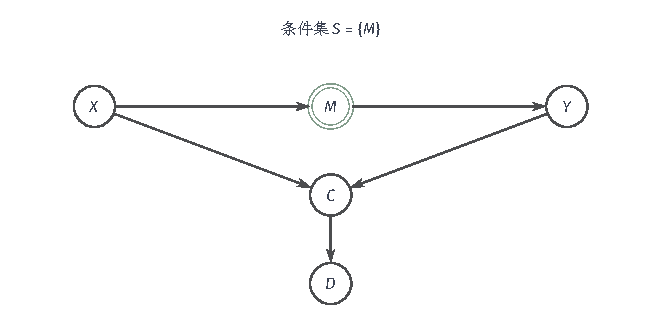
\includegraphics[width=\linewidth]{figures/00-shared/mathematical-preliminaries-lower/01-random-variables-distributions-and-causality/tikz/causal-d-separation-paths/figure.pdf}
  \caption{多条路径下的d-分离。双边框节点\(M\)属于条件集，上方链式路径关闭；
  碰撞点\(C\)及其后代\(D\)都未给定，下方路径也关闭。若再把\(C\)或\(D\)
  加入条件集，下方路径就会打开，说明增加条件可能破坏原有的分离。}
  \label{fig:causal-d-separation-paths}
\end{figure}
\FloatBarrier

图中的阻断只是关于路径的组合判断，尚未自动给出模型分布中的条件独立。若要用图选择调整变量，就需要把这两层接起来：图上已经分离的变量，在模型分布中也应条件独立。下面明确这项由图到概率的要求；随后说明独立外生背景的无环生成模型为何支持它。
\begin{definition}[因果Markov性]
  \label{def:causal-markov-property}
  分布\(P\)相对于因果DAG \(\mathcal G\)满足\term{因果Markov性}
  （causal Markov property），是指对任意两两不交的节点集\(A,B,S\)，
  \[
    A\perp_{\mathcal G}B\mid S
    \quad\Longrightarrow\quad
    \bm V_A\perp\bm V_B\mid\bm V_S.
  \]
  其中\(\bm V_A,\bm V_B,\bm V_S\)分别收集对应节点的随机变量。
\end{definition}

左边是图规则，右边是分布性质。因果Markov性把前者的阻断结论转成条件独立；
它没有说d-连接一定产生统计依赖，也没有从观测独立直接反推箭头。它与时序过程
“给定当前状态后无须更早历史”的Markov性质使用不同对象和条件集，不能只因名称
相同就互相代入。

对DAG，这一全局表述等价于局部表述：每个变量在给定父变量后，与其非后代中除
自身和父变量外的变量条件独立。独立外生噪声的无环SCM满足这一性质。
直观上，非后代及父变量不读取当前节点的独立噪声；给定父变量后，当前变量剩下
的随机性就来自这一噪声。对局部核乘积，按逆向求值次序逐个积分掉无关后代，
每次被消去的条件核积分为一，由此保留所需的局部条件因子。分解与d-分离的
全局对应是DAG的标准结论\scite{math-pearl2009causality}
把图分离转成概率独立，
还需要这里的DAG分解或生成机制条件，不能只凭连接结构推出。
若背景相关而共同来源没有入图，不能仍对这个省略后的DAG直接宣称因果Markov性。

\subsubsection{后门条件下的调整变量选择}
\label{sec:causal-backdoor-selection}

第~\ref{sec:causal-adjustment-identification}节直接假定条件交换性，再证明调整
识别。若已给出具有生成语义的因果图，就可以进一步从路径判断哪些变量可用于调整。这里要保留处理到结果的有向因果作用，并阻断后门准则指定的非因果联系；“有向因果路径”与“后门路径”并不穷尽图上两点间的所有路径。例如\(T\to C\leftarrow U\to Y\)既不是从\(T\)到\(Y\)的有向路径，也不是以箭头进入\(T\)的后门路径；其中碰撞点\(C\)在未被条件化时就阻断了这条路径。因而应先明确路径与阻断的定义，再使用下面的充分准则，不把所有非因果路径都称作后门，也不将有向因果路径另称为前门识别。
从\(T\)到\(Y\)且第一条边指向\(T\)的路径称为
\term{后门路径}（back-door path），它从处理的自然生成来源进入比较，而非沿
处理对结果的有向作用出发。

\begin{definition}[单处理、单结果的后门准则]
  \label{def:causal-backdoor-criterion}
  设\(T,Y\)是因果DAG中的不同节点，\(Z\)与\(\{T,Y\}\)不交。若\(Z\)
  不含\(T\)的后代，且给定\(Z\)阻断所有从\(T\)到\(Y\)、第一条边指向
  \(T\)的路径，则称\(Z\)满足相对于\((T,Y)\)的
  \term{后门准则}（back-door criterion）。
\end{definition}

阻断按定义~\ref{def:causal-d-separation}判断，把碰撞点放进\(Z\)可能打开
原本关闭的路径。最基本的代表图为\(Z\to T,Z\to Y,T\to Y\)，独立噪声机制给出
\[
  p(z,t,y)=p(z)p(t\mid z)p(y\mid t,z).
\]
将处理机制替换为常量\(t\)后，
\(p(z,y\mid\operatorname{do}(T=t))=p(z)p(y\mid t,z)\)。再对背景积分，得到
\begin{equation}
  p(y\mid\operatorname{do}(T=t))
  =
  \int p(y\mid t,z)p(z)\,\mathrm dz.
  \label{eq:causal-backdoor-adjustment}
\end{equation}
离散背景用求和，一般空间用对\(P_Z\)的核积分。对结果再取期望，就回到
式~\eqref{eq:causal-g-formula}的调整表示。

一般后门准则在独立噪声无环SCM、图正确包含相关共同原因且干预保留其他机制的
条件下，给出同样的调整结论\scite{math-pearl2009causality}
阻断全部后门路径排除了自然处理选择沿这些路径携带的背景差异，非后代条件保证
用于平均的\(Z\)不先被行动改变。这些是生成结构对交换性的充分支持，而不是只由
一个观测分布满足Markov性就能推出的干预结论。即使图条件成立，要从观测资料
确定积分中的局部响应，还需要目标总体内所用处理的支持条件；图不会填补空白
协变量--处理组合。

三个局部图可以核对变量角色。在\(T\leftarrow X\to Y\)中，\(X\)关闭后门；
在\(T\to M\to Y\)中，\(M\)是后代，固定它会改变总效应目标；
在\(T\to C\leftarrow Y\)中，空条件集已经关闭碰撞路径，加入\(C\)反而打开它。
因此，处理前测量、与结果相关或能提高预测精度，都不是充分的调整标准。

下面用三个小算例分别核对这些角色。先在\(T\to C\leftarrow Y\)中取\(T\)与
\(Y\)独立，各以概率\(1/2\)取\(0\)或\(1\)，并令\(C=T\oplus Y\)（两者
相同时为\(0\)，不同时为\(1\)）。无条件时\(\mathbb P(T=1\mid Y=1)=1/2\)，
两者没有关联；但在\(C=1\)子群中，\(\mathbb P(T=1\mid Y=1,C=1)=0\)。
这是因为筛选只留下\((T,Y)=(0,1),(1,0)\)两类记录，原本独立的变量在这个
子群内成为完全负相关。

子群关联还应与按全部\(C\)层标准化的总体量区分。记层内均值差为
\(\delta_c=\mathbb E[Y\mid T=1,C=c]-\mathbb E[Y\mid T=0,C=c]\)。
在\(C=0\)层有\(Y=T\)，在\(C=1\)层有\(Y=1-T\)，因此
\[
  \delta_0=1-0=1,\qquad \delta_1=0-1=-1.
\]
两层的概率各为\(1/2\)，所以若仿照调整式对它们平均，得到
\[
  \sum_{c\in\{0,1\}}\mathbb P(C=c)\delta_c
  =\frac12\times1+\frac12\times(-1)=0.
\]
这个模型中改变\(T\)只改变\(C\)，不改变\(Y\)的规则，真实总效应也是零。
该算例说明的是在\(C=1\)子群中筛选会制造关联，没有展示总体调整后的偏差或
效应符号反转。这里的正负相消也不能用来保证一般模型中按碰撞点调整仍然有效；
图上路径一旦打开，原来的独立性保证就已失去。

再看中介图\(T\to M\to Y\)。令\(T\sim\operatorname{Bernoulli}(1/2)\)，
噪声\(\eta,\varepsilon\)均为标准正态，且\(T,\eta,\varepsilon\)相互独立，
机制为\(M=T+\eta\)、\(Y=M+\varepsilon\)。设置\(T=t\)后，中介随处理重新
生成，故
\[
  Y(t)=t+\eta+\varepsilon,\qquad
  \mathbb E[Y(t)]=t,\qquad \tau=1.
\]
若改为按观测中介\(M=m\)分层，则由\(\varepsilon\)独立于\((T,M)\)且均值
为零，得到
\[
  \mathbb E[Y\mid T=t,M=m]
  =m+\mathbb E[\varepsilon\mid T=t,M=m]=m.
\]
这里使用该连续密度模型给出的条件均值版本。给定任一处理，\(M\)的正态密度在
每个实数\(m\)处均为正，因此两种处理在这些中介取值附近都有记录；不要求精确
事件\(\{M=m\}\)本身有正概率。层内两组均值差为\(m-m=0\)，而总效应为\(1\)：
固定中介没有保留处理经中介传递的作用。

“按观测\(M\)分层”与“主动同时设定\(T,M\)”仍是不同操作。若研究的是联合干预
\(\operatorname{do}(T=t,M=m)\)，本例得到\(Y=m+\varepsilon\)，故固定同一
\(m\)时的受控处理效应也为零。这个数值一致依赖当前机制与独立噪声，不能据此
把观测条件化和联合干预一般地等同。估计总效应时，要让中介按各处理下的规律变化。

最后在纯共同原因图\(T\leftarrow X\to Y\)中，明确给出二元处理的分配机制。
令\(X\sim\operatorname{Bernoulli}(1/2)\)、\(W\sim\operatorname{Unif}(0,1)\)
和标准正态噪声\(\zeta\)相互独立，并设
\[
  T=\mathbf 1\{W\leq0.2+0.6X\},\qquad Y=2X+\zeta.
\]
于是\(e(0)=0.2,e(1)=0.8\)，每个\(X\)层内的两种处理都有正概率。
Bayes公式给出\(\mathbb P(X=1\mid T=1)=0.8\)、
\(\mathbb P(X=1\mid T=0)=0.2\)，故
\[
  \begin{aligned}
    \mathbb E[Y\mid T=1]&=2\times0.8=1.6,\\
    \mathbb E[Y\mid T=0]&=2\times0.2=0.4.
  \end{aligned}
\]
观测差为\(1.2\)，来自两组\(X\)构成的差异。按\(X\)分层则有
\(\mathbb E[Y\mid T=t,X=x]=2x\)，所以每层均值差为零，调整后为
\[
  \sum_{x\in\{0,1\}}\mathbb P(X=x)(2x-2x)=0.
\]
直接核对干预也得到同一答案：替换处理规则不改变\(X\)和\(Y\)的机制，
\(Y(t)=2X+\zeta\)的均值恒为\(1\)，因而真实总效应为零。这个完整构造才允许
把观测差归于共同原因；仅有两组均值不同并不足以作这种归因。

在上述特定图中估计总效应，共同原因\(X\)可用于层内比较并按同一总体权重平均；
中介\(M\)应随处理重新生成，以保留间接作用；按碰撞点\(C\)筛选可能制造关联。
一般情况下，调整集合的选择仍取决于完整因果图、所求总效应或直接效应，以及
所用识别方法，必须检查全部相关路径和处理支持，不能只按变量名称决定。
后门准则是充分条件，不是识别的必要条件；它不适用时，随机设计、其他识别规则
或更具体的机制假设仍可能确定所选目标。

\section{因果生成结构的推断}
\label{sec:causal-structure-discovery}

给定图与局部机制，可以从背景逐步生成结果。反过来，仅看到结果记录时，需要辨认两类未知：一是变量之间的关系结构——谁是因、谁是果，哪些变量进入同一条方程；二是在结构已经给定时，每条局部方程的具体形式、参数和噪声规律。关系推断改变候选图，机制推断改变给定图上的函数和噪声；两项都会影响最终算出的响应。需要强调的是，把联合分布拟合得再好，通常也只能说明候选模型与观测相容，并不能唯一确定箭头方向或同一个体的反事实，这些还需要干预、环境变化或额外结构假设。

\subsection{变量关系的推断}
\label{sec:causal-relation-inference}

从图推出分布约束与从分布反推图，是方向相反的两项任务。要用条件独立排除候选
关系，需要说明哪些独立是真正的结构阻断，哪些可能来自参数抵消。还要说明记录
来自同一观测环境、受控干预还是不同环境，因为这些资料对候选机制提供的限制不一样。

\subsubsection{观测资料下的关系识别}
\label{sec:causal-observational-structure}

前面在生成假设下从图上分离推出分布中的条件独立。结构推断需要反向使用这些约束：给定可观测分布时，检查哪些候选图与它的条件独立关系相容；只有有限观测记录时，则还需估计和检验这些关系，不能把未检出依赖直接当成精确独立。反向使用独立约束还须排除参数抵消等巧合，即图上没有分离的变量却在相应条件分布中独立。下面的忠实性假设要求这些分布独立关系都能由图结构解释，而不是由特定参数抵消产生。
\begin{definition}[相对于DAG的忠实性]
  \label{def:causal-faithfulness}
  分布\(P\)相对于DAG \(\mathcal G\)满足\term{忠实性}（faithfulness），若对
  任意两两不交的节点集\(A,B,S\)，
  \[
    \bm V_A\perp\bm V_B\mid\bm V_S
    \quad\Longrightarrow\quad
    A\perp_{\mathcal G}B\mid S.
  \]
\end{definition}
忠实性要求分布中出现的条件独立能由图结构解释，不是由特殊参数抵消、确定性
约束或未处理的误差相关造成。因果Markov性给出正向蕴含，忠实性补上反向蕴含，
两者不能互相替代。

例如，设\(X,U_M,U_Y\)相互独立，
\(M=\alpha X+U_M\)，\(Y=\beta X+\gamma M+U_Y\)。
当\(\alpha,\gamma\ne0\)且\(\beta=-\gamma\alpha\)时，
\(Y=\gamma U_M+U_Y\)与\(X\)独立，但图中直接路径\(X\to Y\)及
\(X\to M\to Y\)都存在。两条贡献恰好抵消，说明无环与独立噪声并不自动保证
忠实性。接近这种抵消时，非零依赖还可能非常弱，有限样本中难以检出。

只考察三个节点且没有其他路径时，链
\(X\to Z\to Y\)、反向链\(X\leftarrow Z\leftarrow Y\)和共同原因
\(X\leftarrow Z\to Y\)都蕴含
\[
  X\perp Y\mid Z,
\]
却一般不蕴含\(X\perp Y\)。条件独立模式无法区分中间变量在传递作用还是造成
共同变化。碰撞结构\(X\to Z\leftarrow Y\)则蕴含\(X\perp Y\)，给定中间
节点后可能相关；加上忠实性，才能把这种模式差别用作反向辨识的依据。
这三种结构回用图~\ref{fig:causal-local-path-patterns}的路径规则；加入其他节点和边以后，独立判断仍须遍历全部相关路径。

\begin{definition}[Markov等价与等价类]
  \label{def:causal-markov-equivalence}
  同一节点集上的两张DAG若具有完全相同的d-分离关系，就称它们
  \term{Markov等价}（Markov equivalent）。
  与给定图Markov等价的全部DAG组成其
  \term{Markov等价类}（Markov equivalence class, MEC）。
\end{definition}

图的\term{骨架}（skeleton）是忽略箭头方向后的邻接关系。
\term{无屏蔽碰撞结构}（unshielded collider）指
\(X\to Z\leftarrow Y\)，并且两端\(X,Y\)不相邻。没有两端的直接边，才使
这个局部碰撞的差异能够通过两端的分离关系表现出来。
标准判据是：两张DAG Markov等价，当且仅当具有相同骨架和相同无屏蔽碰撞结构
\scite{pgm-structure-learning-chickering2002}

判据的必要性可以直接从全部路径证明。先说明DAG中任意两个非相邻节点都有一个
不含端点的d-分离集。选其中一个节点\(v\)，使另一个节点\(w\)不是它的后代；
无环性保证至少有这样一个选择。令条件集为\(v\)的父节点集。
任意从\(v\)到\(w\)的路径若第一条边指向\(v\)，就经过一个父节点；因两端
不相邻，该父节点是内部非碰撞点，路径被阻断。
若第一条边从\(v\)向外，路径不可能一直沿箭头到达非后代\(w\)。沿路径第一次
改变箭头方向时，出现一个碰撞点\(c\)，此前的有向前缀说明\(c\)是\(v\)的
后代。\(c\)及其任何后代都不可能成为\(v\)的父节点，否则形成有向环；
故这个碰撞点没有被条件集打开，路径仍被阻断。两类覆盖了全部路径。
相邻节点之间的单边路径则没有内部点，不可能被任何不含端点的条件集阻断。
因此，骨架不同必导致d-分离关系不同。

再考虑同一骨架上的无屏蔽三点结构\(X-Z-Y\)。两端不相邻，按上段存在分离集。
若\(Z\)不是碰撞点，任何分离集都必须包含\(Z\)，否则长度为二的这条路径
仍然活跃；若\(Z\)是碰撞点，任何分离集都不能包含\(Z\)，否则该路径被打开。
因此，中点碰撞状态不同也必然改变d-分离关系。其他路径可能增加分离要求，却
不会消除这条长度为二的路径对每个分离集施加的限制。

充分性需要控制所有较长路径，这里引用完整结构判据，不把上述必要性论证冒充
双向证明\scite{pgm-structure-learning-chickering2002}
理解等价类内部的方向变化还可借助\term{覆盖边}（covered edge）：边
\(X\to Y\)若满足
\[
  \operatorname{pa}(Y)=\operatorname{pa}(X)\cup\{X\},
\]
便是覆盖边，这里\(\operatorname{pa}(X)\)表示父节点集合。
覆盖边反转定理说明，反转这种边后仍为DAG，并保持全部d-分离关系
\scite{pgm-structure-learning-chickering2002}
从局部因子看，在前述共同参考测度下的密度表示中，对给定共同父变量，这一步把
\[
  p(x\mid\operatorname{pa}(X))
  p(y\mid x,\operatorname{pa}(X))
  =
  p(y\mid\operatorname{pa}(X))
  p(x\mid y,\operatorname{pa}(X))
\]
重新分解，不改变两变量的条件联合分布。因子应取相容的条件版本；这个等式解释
分布重参数化，却没有单独证明全图等价，更没有证明两张指定图之间存在变换序列。
完整变换定理进一步保证，任意两张已知Markov等价的DAG，可以经有限次覆盖边
反转相互到达，每个中间图都保持无环且等价。这是等价类内的可达性结论，不能
代替结构判据的充分性证明\scite{pgm-structure-learning-chickering2002}

等价类可以用部分有向图表示：全部等价图都同意的方向保留箭头，其余边保持无向。
在因果Markov性、忠实性、无环和无潜在混杂等条件下，纯观测条件独立信息一般
只能识别这样的等价类。输出一条无向边并非一定表示算法未完成；它可能记录总体
观测分布本身无法决定的方向。

这种“方向确实无法确定”可以用三个二元变量算出来。取
\(\mathbb P(X=1)=0.4\)，\(\mathbb P(Z=1\mid X=0)=0.2\)、
\(\mathbb P(Z=1\mid X=1)=0.7\)，
\(\mathbb P(Y=1\mid Z=0)=0.1\)、\(\mathbb P(Y=1\mid Z=1)=0.6\)，
按链\(X\to Z\to Y\)计算联合分布，再把中间的因子按Bayes公式重排成
\(Z\to X\)与\(Z\to Y\)，得到的八个联合概率逐一相同。
两套机制给出同一个观测分布，却对“改变\(X\)会不会改变\(Y\)”给出相反答案：
在前一套中\(X\)影响\(Y\)，在后一套中\(X\)与\(Y\)只是共同受\(Z\)影响。
观测数据无论多少都不能区分它们，必须靠干预或环境变化提供额外信息。
这不是算法精度问题，而是可识别性本身的边界。

这里还隐含了变量覆盖。相对于所选观测节点集，若这些节点之间的共同原因都已纳入，
不存在未记录的共同原因，就称满足因果充分性（causal sufficiency）。
这是全节点范围的要求；仅针对特定处理与结果排除未观测混杂，并不足以保证
其他观测节点之间也没有隐藏共同原因。
潜在共同原因能让两个可观测节点相关，却不应被硬解释成其中一个直接导致另一个。
允许潜在混杂或选择后，输出往往需要扩大到带不同端点标记的部分图，分别表示
已确定的祖先关系、可能方向和无法排除的隐藏共同原因。测量误差以及按碰撞点
选择样本也会改变独立模式，不应一律视为新增因果边。

有限样本中的关系发现还要通过检验或评分近似总体判断。以
\(H_0:V_i\perp V_j\mid\bm V_S\)为原假设，若约束型算法在未拒绝独立时
删除候选边，那么第一类错误把真实独立误判为依赖，可能保留虚假边；
第二类错误把实际依赖误判为独立，可能删除真实边。后续搜索与定向会传播错误，
评分型算法则不能直接套用这组对应。高维条件集减少每层有效样本，近忠实边界上
的弱依赖尤其难判断。结构学习的一致性必须同时说明总体的Markov与忠实条件、
检验或评分的渐近性质、候选图范围，以及搜索能否达到目标；一张确定输出图
不代表因果方向已经唯一。

\subsubsection{干预与环境变化下的方向识别}
\label{sec:causal-interventional-structure}

要打破观测方向歧义，需要增加具有不同约束的信息。理想干预切断目标变量的原
进入机制：若随机设置\(X\)后，\(Y\)的分布随设置值改变，在其余机制不变、
行动确实只作用于\(X\)的模型中，这支持\(X\)位于\(Y\)的上游。反之，没有
观察到分布改变并不自动排除作用，机制抵消、剂量范围或检验能力都可能影响判断。
对多个节点施加适当干预可缩小观测等价类，但能缩小到什么程度取决于干预覆盖。

这一证据必须按实际执行解释。干预目标未知、执行不完全，或干预同时改变测量、
选择和其他机制时，都应将这些不确定性纳入模型。不能把“鼓励参加培训”无条件
等同于“把培训处理设为指定值”，也不能把伴随整套制度改变的干预解释成单个
节点的理想替换。

不同环境也可能提供方向限制。设环境标签为\(E\)，若假定环境只改变输入\(X\)
的分布，而机制\(Y=f_Y(X,U_Y)\)及独立噪声\(U_Y\)的分布保持不变，那么
各环境在共同支持上的\(P(Y\mid X,E=e)\)应相同；反向条件分布
\(P(X\mid Y,E=e)\)却可能随输入分布变化。这里稳定性来自已声明的生成假设，
并非看到一个稳定条件分布就证明了箭头。

潜在共同原因可以在所有已观察环境中稳定，环境变化也可能太弱，未能打破错误
方向；选择规则同步变化还可能制造稳定关联。应分别说明哪些背景分布或局部
机制允许改变，哪些保持不变，环境是否直接影响结果，以及稳定性究竟是模型
假设、检验对象还是经验线索。机制知识和对隐藏混杂、弱依赖、选择过程的
敏感性分析，共同限制候选关系，不能由增加同分布样本替代。

对于反馈环、随时间改变的机制或处理定义不稳定的系统，无环静态模型本身可能
不合适，需要改用动态或循环模型并重新定义行动；方向识别不能先忽略模型边界，
再用搜索算法的精度弥补。

\subsection{局部机制的推断}
\label{sec:causal-local-mechanism-inference}

即使关系已经给定，箭头也没有给出作用大小、非线性形状和背景分布。
局部机制推断要在声明的函数族、噪声条件和观测制度内估计这些未知部分。
它可以回用第~\ref{sec:rv-inference}节的有限维参数或函数估计，但必须先明确
估计对象是否具有所需的干预含义。

例如，对已给定的父变量向量\(\bm P_j\)，假设局部方程为
\[
  V_j=\theta_{j0}+\bm\theta_j^{\mathsf T}\bm P_j+\varepsilon_j,
  \qquad
  \mathbb E[\varepsilon_j\mid\bm P_j]=0.
\]
令\(\bm Z_j=(1,\bm P_j^{\mathsf T})^{\mathsf T}\)，并令
\(\bm\vartheta_j=(\theta_{j0},\bm\theta_j^{\mathsf T})^{\mathsf T}\)。
若二阶矩有限且
\(\bm Q_j=\mathbb E[\bm Z_j\bm Z_j^{\mathsf T}]\)可逆，乘以\(\bm Z_j\)再取
期望得到
\[
  \mathbb E[\bm Z_jV_j]=\bm Q_j\bm\vartheta_j,\qquad
  \bm\vartheta_j
  =\bm Q_j^{-1}\mathbb E[\bm Z_jV_j].
\]
因此在这些条件下，局部参数可由总体矩识别。独立同分布样本中的对应矩估计为
\[
  \widehat{\bm\vartheta}_j
  =
  \left(\frac1n\sum_{i=1}^n\bm Z_{ij}\bm Z_{ij}^{\mathsf T}\right)^{-1}
  \left(\frac1n\sum_{i=1}^n\bm Z_{ij}V_{ij}\right),
\]
前提是样本矩可逆。误差、区间和正则化处理仍属于统计估计问题。真实父变量
存在确定性共线时，矩方程不能唯一确定各系数；遗漏共同背景造成条件噪声均值
非零时，拟合得到的斜率也不再自动等于局部结构参数。

在培训例子里，可以分别拟合技能方程和成绩方程，再复合为
\(\widehat\beta+\widehat\gamma\widehat\alpha\)。结果方程中的
\(\widehat\beta\)只是固定技能时的局部系数，不应独自报告为总效应。这样从
局部估计传到整体响应时，还须传播多个估计量的共同误差。

非参数情形也要区分三个层次。观测资料可以在父变量支持上估计
\(P(V_j\mid\operatorname{pa}_j)\)；把这个条件核解释为干预下保持不变的机制，
还需要正确关系、噪声及机制不变假设；再要求同一背景下不同输入怎样配对，则
需要更强的结构表示。同一组局部条件核可以由不同结构函数和背景耦合实现。
第~\ref{sec:causal-factual-counterfactual}节的两种跨世界配对已经说明，边缘
分布相同不决定已知事实后的替代结果。因此，仅拟合条件分布不能自动唯一恢复
个体响应、反事实公平或行动成功概率。

即使所有观测和干预分布都已确定，结构函数与背景仍可能有多种等价表示，因此一般SCM未必能够唯一恢复。加性独立噪声、特定函数形状和支持外的平滑性会缩小候选范围；它们应作为明确假设参与识别分析。模型在已有支持内拟合良好，只检验了这些记录上的概率预测。支持外行动的响应仍依赖外推，背景独立与机制不变也需要各自的依据。

实际可保留候选模型\((\mathcal G,\{f_j\},P_{\bm U})\)，逐一生成所关心的响应，
再把这些答案送回第~\ref{sec:causal-partial-identification-sensitivity}节的
识别集合。关系不确定、局部参数或函数不确定、跨世界背景配对不确定可能贡献
不同范围；样本有限还会增加估计误差。把这些来源分别传到平均效应、策略价值
或补救约束，才不会用一个最优拟合模型掩盖其他同样相容的行动后果。

\section{本章小结}
\label{sec:causal-inference-summary}

开篇的培训问题不能只由两组成绩差回答，因为自然接受处理的人可能具有不同背景。
给定生成模型和背景分布以后，响应映射能计算主动改变处理的后果；得知某人的事实
以后，则先更新背景分布，再在同一背景下改变行动。前者改变生成规则，事实条件化
改变对背景的认识，两步不能混成从干预总体重新抽一个人。

响应比较有不同口径。同背景之差描述个体效应，对目标总体平均得到ATE，对处理前
信息分层得到CATE，比较完整边缘分布可以保留均值以外的变化，连续处理的导数则
描述局部变化。平均相同不表示无人受益或受损，干预边缘相同也不决定跨世界配对。
补救要同时声明目标、可行动变量、成本与成功保证；公平约束还须明确同背景的属性
比较及其规范含义。

能够在模型内计算，不等于能够由资料识别。明确的处理版本、一致性和无干扰使目标
与实际记录相连，随机分配或条件交换性支持响应识别，支持条件保证资料覆盖目标
会使用的协变量--行动组合。调整与逆概率表示是同一目标的不同表达。结构图建立后，
后门准则为某些调整选择提供充分依据，却不能代替目标支持，也不是全部识别方法的
必要前提。

无法点识别时，有界结果、支持缺口和敏感性约束保留所有相容答案。单调性、效应
范围、外推或跨环境稳定可以缩小模型类，但收紧来自这些新增条件。一般识别集合
不必是区间，有效包络也不自动是锐界。识别范围描述总体机制歧义，统计区间描述
有限样本误差，积分与优化还有各自的数值误差。增加同分布样本主要改善估计；
受控干预、扩大行动覆盖或增加可辩护的机制知识，才可能减少原有识别歧义。
缩小目标人群可以改善覆盖，却也改变了要回答的问题。

无环SCM把局部函数复合成唯一可测的自然及干预响应，图记录这些函数的输入关系。
对固定计算模型的受控替换，可以据此计算输入或中间读数改变后的输出；这种程序内
比较是否代表现实因果效应，仍取决于两者的变量与生成机制能否对应。
因果Markov性从图推出独立约束，忠实性允许反向使用独立信息；纯观测结构发现
通常止于Markov等价类，潜在混杂、选择和测量误差还会改变候选范围。关系确定后
仍须推断局部机制，观测条件分布拟合又不自动确定同背景反事实。因此每项结论都
应列明目标、行动定义、生成假设、资料制度和剩余不确定性。

路径、分离和结构分解为这里的图判断提供计算工具，图本身的因果解释则来自本章的
机制假设。

从单步策略转向连续行动时，前一步的结果会影响下一步的条件，还需要描述这些作用
怎样逐步生成轨迹。\BookChapterRef{chap:dynamical-systems-and-state-estimation}{第~\ref{chap:dynamical-systems-and-state-estimation}章}先给定状态更新
机制、输入与噪声规律，研究状态的演化；\BookChapterRef{chap:control-theory}{第~\ref{chap:control-theory}章}再考察观测和执行
限制下的策略实现。
\BookSectionRef{sec:decision-dynamic-programming}{第~\ref{sec:decision-dynamic-programming}节}将单步策略扩展到历史和序贯价值，
需要重新检查时变混杂、逐时支持与轨迹目标。
后续公平与解释专题分别回用反事实公平和行动补救，并补充规范要求与现实验证条件。

